\documentclass[12pt, a4paper, oneside]{book}


%------------------------
% IMPORT PACKAGES
%-----------------------
\usepackage{amsthm}
\usepackage{mathtools}
\usepackage{algpseudocode}
\usepackage[chapter]{algorithm}
\usepackage{amssymb}
\usepackage{graphicx}
\usepackage{caption}
\usepackage{fancyvrb}
\usepackage{array}
\usepackage[acronym,toc,nohypertypes={acronym,notation},nonumberlist,automake]{glossaries}
%\usepackage{hyperref}
\usepackage{epigraph}
\usepackage{url}
\def\UrlBreaks{\do\/\do-}
\usepackage{breakurl}
\usepackage[breaklinks]{hyperref}
\expandafter\def\expandafter\UrlBreaks\expandafter{\UrlBreaks%  save the current one
	\do\a\do\b\do\c\do\d\do\e\do\f\do\g\do\h\do\i\do\j%
	\do\k\do\l\do\m\do\n\do\o\do\p\do\q\do\r\do\s\do\t%
	\do\u\do\v\do\w\do\x\do\y\do\z\do\A\do\B\do\C\do\D%
	\do\E\do\F\do\G\do\H\do\I\do\J\do\K\do\L\do\M\do\N%
	\do\O\do\P\do\Q\do\R\do\S\do\T\do\U\do\V\do\W\do\X%
	\do\Y\do\Z}
\usepackage{listings}
\usepackage{systeme}
\usepackage{cancel}
\usepackage{color}
\usepackage[table, dvipsnames]{xcolor}
\usepackage{tikz}
\usepackage{subcaption}
\usepackage{dsfont}

\usepackage{booktabs}
\usepackage{makebox}

\usepackage{lipsum}


\usepackage{IEEEtrantools}

\usepackage{cleveref}



\DeclareMathOperator*{\argmax}{arg\,max}
\DeclareMathOperator*{\argmin}{arg\,min}

%% remark theoremstyle
%\newtheoremstyle{break}
%{\topsep}{\topsep}%
%{\itshape}{}%
%{\bfseries}{}%
%{\newline}{}%
%\theoremstyle{break}
%\newtheorem{remark}{Remark}[section]

% problem theoremstyle
%\newtheoremstyle{problemstyle}  % <name>
%{10pt}  % <space acbove>
%{10pt}  % <space below>
%{\normalfont} % <body font>
%{}  % <indent amount}
%{\bfseries\itshape} % <theorem head font>
%{\normalfont\bfseries:} % <punctuation after theorem head>
%{.5em} % <space after theorem head>
%{} % <theorem head spec (can be left empty, meaning `normal')>
%\theoremstyle{problemstyle}
%\newtheorem{problem}{Problem}[section] % Comment out [section] toremove section number dependence
%\newtheorem{definition}{Definition}[section]
%\newtheorem{theorem}{Theorem}[section]
%\newtheorem{proposition}{Proposition}[section]
%\newtheorem{remark}{Remark}[section]
%\newtheorem{lemma}{Lemma}[section]
% create command for variance in math mode
%\newcommand{\Var}[1]{\operatorname{Var}\left[#1\right]}
%\newtheorem{thm}{Theorem}[section]
%\newtheorem{mydef}{Definition}[section]
%\newtheorem{myexample}{Example}[section]
%\newtheorem{myprop}{Proposition}[section]

%\newcommand{\source}[1]{\caption*{Source: {#1}} }

%\renewcommand\textflush{flushright}
\setlength\epigraphwidth{.6\textwidth}


%\newacronym{EC}{EC}{Elliptic Curve}
%\newacronym{ECC}{ECC}{Elliptic Curve Cryptography}
\newacronym{i.i.d}{i.i.d}{Independent and identically distributed}
\newacronym{RCLL}{RCLL}{Right continuous with left limit}
\newacronym{SV}{SV}{Stochastic Volatility}
\newacronym{JD}{JD}{Jump Diffusion}
\newacronym{GBM}{GBM}{Geometric Brownian Motion}
\newacronym{PDE}{PDE}{Partial Differential Equation}
\makeglossaries


\definecolor{dkgreen}{rgb}{0,0.6,0}
\definecolor{gray}{rgb}{0.5,0.5,0.5}
\definecolor{mauve}{rgb}{0.58,0,0.82}

\lstdefinestyle{mystyle}{
	backgroundcolor=\color{gray!30},   
	commentstyle=\color{green},
	keywordstyle=\color{blue},
	numberstyle=\tiny\color{gray},
	stringstyle=\color{black},
	basicstyle=\footnotesize,
	breakatwhitespace=false,         
	breaklines=true,                 
	captionpos=b,                    
	keepspaces=true,                 
	numbers=left,                    
	numbersep=5pt,                  
	showspaces=false,                
	showstringspaces=false,
	showtabs=false,                  
	tabsize=2
}

\lstset{style=mystyle}

\begin{document}

%----------------------------------------------------------------------------------------
% COVER PAGE
%----------------------------------------------------------------------------------------
\pagestyle{empty}
\begin{titlepage}

	\begin{center}
		\normalsize 
			\textsc{Politecnico di Milano}\\
			School of Industrial and Information Engineering\\
			Master of Science in Mathematical Engineering\\

	\end{center}
	\vspace{.6cm}
	
	\begin{figure}[htpb]
		\centering
		
\includegraphics[width=4cm]{Cover/polimi}
	\end{figure}
	\vspace{.6cm}
	
	\begin{center}
		\LARGE
			\textsc{TITLE: very interesting subject, ain't it?}
	\end{center}
	\vspace{1.6cm}

	\begin{flushleft}
		\large
		\begin{tabular}{ll}
		Supervisors:    & Prof. Daniele Marazzina      \\
		             		   & Prof. Ferdinando M. Ametrano
		\end{tabular}
		\vspace{1cm}
	\end{flushleft}
	
	\begin{flushright}
		\large
		Master thesis by:\\
		Samuele Vianello\\
		ID: *********\\		
	\end{flushright}
	
	\vspace*{\fill}
	\begin{center}
		Academic year 2017-2018
	\end{center}
	
\end{titlepage}


%----------------------------------------------------------------------------------------
% ABSTRACT
%---------------------------------------------------------------------------------------

%% Set page numbers of the introduction to roman  
\frontmatter
\pagestyle{plain}
%\chapter{Abstract}
\label{chpr:abstract}

Bitcoin is increasingly establishing itself as a digital investment asset other than a mere speculative instrument. In this work, we explore this subject by studying the correlation that Bitcoin has with other standard assets such as stock and bond indexes,  currencies and commodities. We first study the empirical correlation and its statistical significance, then calibrate more sophisticated asset models including jump diffusion and stochastic volatility in their multivariate generalizations to obtain the correlation matrices also under those frameworks. Results are closely related and Bitcoin correlation  with any other asset is confirmed to be very low. Given this result, we perform optimal portfolio allocation analyses to investigate its diversification properties, both through Markowitz mean-variance optimization and using the CVaR as the portfolio risk measure. Evidence shows that allocating a small percentage of wealth in the digital assets proves to be extremely beneficial in terms of lowering the risk and increasing the expected returns.




%\cleardoublepage
%\vspace*{\fill}
%\epigraph{\textit{The secret to happiness is freedom. \\ And the secret to freedom is courage.}}{Thucydides}
%\vspace*{\fill}


%----------------------------------------------------------------------------------------
%	LIST OF CONTENTS/FIGURES/TABLES PAGES
%----------------------------------------------------------------------------------------

\tableofcontents
\listoftables
\addcontentsline{toc}{chapter}{List of Tables}
\listoffigures
\addcontentsline{toc}{chapter}{List of Figures}


\glsaddall
\printglossaries

\chapter{Abstract}
\label{chpr:abstract}

Bitcoin is increasingly establishing itself as a digital investment asset other than a mere speculative instrument. In this work, we explore this subject by studying the correlation that Bitcoin has with other standard assets such as stock and bond indexes,  currencies and commodities. We first study the empirical correlation and its statistical significance, then calibrate more sophisticated asset models including jump diffusion and stochastic volatility in their multivariate generalizations to obtain the correlation matrices also under those frameworks. Results are closely related and Bitcoin correlation  with any other asset is confirmed to be very low. Given this result, we perform optimal portfolio allocation analyses to investigate its diversification properties, both through Markowitz mean-variance optimization and using the CVaR as the portfolio risk measure. Evidence shows that allocating a small percentage of wealth in the digital assets proves to be extremely beneficial in terms of lowering the risk and increasing the expected returns.



%\chapter{Acknowledgements}
\label{chpr:acknowledgement}

***add acknowledgements***

\bigskip
\noindent

\bigskip 
\noindent
Thank you.


%----------------------------------------------------------------------------------------
%	THESIS CONTENT - CHAPTERS
%----------------------------------------------------------------------------------------

\mainmatter

\chapter{Introduction}
\label{chpr:intro}

\bigskip


Bitcoin was presented in \citep{BTC2008} as a peer-to-peer protocol for electronic cash that would allow online payments to be sent directly from one party to another without going through a financial institution.
It started off in 2009 as system that was only used by a niche of people in online cryptology forums  to experiment with the transaction protocol. It took a few years for Bitcoin to gain public notoriety, while the price kept rising and having quick crashes. 

Bitcoin generated a lot of buzz in 2017, a year that registered the price increase from 998 \$ to 13,412 \$ in January 2018 with an all-time high of 19,666 \$ on the 17th of December. Since then, the price has deflated to a level of six thousand dollars in 2018 and has lately stabilized around three thousands.

Setting aside the mere numerical value of the price, Bitcoin was the first protocol to solve the problem of double-spending without the need for a centralized party: bitcoins can be transferred but not duplicated, as they only exist as validated transaction in the distributed blockchain. 
These features allow Bitcoin to have a chance at becoming a global, instantaneous and free payment network that would make wealth transfer as easy as online data sharing.
In the same way that e-mail substituted post mail, Wikipedia and other knowledge-based website outdated paper encyclopaedias, music and film streaming services are becoming the new user friendly experience for the two industries, Bitcoin presents itself as a system to exchange wealth between users without the need for banks or other trusted third parties.

Furthermore, Bitcoin is the first digital currency to achieve scarcity in the digital realm: its monetary policy based on deterministic supply mimics the progressive scarcity of gold. For these reasons we believe that Bitcoin  is \textit{digital gold} with an embedded secure network and its characteristics make it resemble more closely a crypto-asset rather than a crypto-currency.
Even though there are a number of supporters of this idea, for instance in \citep{DYHRBERG2016} it is shown that Bitcoin possesses the same hedging abilities of gold, there is no general consensus on the matter and different studies get to the opposite result: see for example \citep{KLEIN2018}.

Bitcoin has been called many names: a bubble, a Ponzi scheme, it has been defined as sound money and store of value. We agree with the latter and believe that if Bitcoin is a true digital gold, then its value will express the huge potential that has been so far limited by scepticism and misunderstandings.

\bigskip

In the present work, we intend to first study the correlation that exists between Bitcoin and other types of standard assets, both by analysing the empirical correlation of the returns and by calibrating more sophisticated models such as \text{jump diffusion} and \textit{stochastic volatility} models.
Secondly, we want to explore the diversification property of adding Bitcoin to a portfolio of asset, by computing the optimal allocation for different levels of risk and expected return.


\bigskip
\noindent
The present thesis has been written during the author's fellowship at the Digital Gold Institute, a research and development center focused on teaching, consulting, and advising about scarcity in the digital domain (Bitcoin and crypto-assets) and the underlying blockchain technology. \\
The interested reader can visit the webpage of the institute at the link: \href{https://www.dgi.io/}{https://www.dgi.io/}.

\bigskip

\section{Thesis structure}
Our work is structured into 5 chapters.

\bigskip
\noindent
In Chapter \ref{chpr:corr_analysis} we study the empirical correlation between the assets taken into considerations(Section \ref{emp_corr}). We also take a look at the significance of each correlation value by performing two statistical tests, Pearson's \textit{t}-test and a permutation test, in Section \ref{sec:corr_significance}. Finally, Section \ref{sec:rolling_cor} investigate the rolling correlation between Bitcoin and the other assets.

\bigskip
\noindent
In Chapter \ref{chpr:models} we present each model that we are going to adopt in our work. We first give a brief overview of the building blocks necessary to understand the mathematical framework of the models: definitions of geometric Brownian motion, compound Poisson process and CIR process are all presented in Section \ref{sec:notions}. 
In the following sections we consider the models themselves. We  present the univariate formulations of Merton (Section \ref{sec:merton}), Heston (Section \ref{sec:heston}) and Bates (Section \ref{sec:bates}) and provide a possible generalization to the multi-asset case following the parsimonious approach presented in \citep{PARSIMONIOUS2011}

\bigskip
\noindent
In Chapter \ref{chpr:calibration} we explain how to calibrate each different model: first we present a general overview of the maximum likelihood estimation (Section \ref{sec:calib_overview}) and then we proceed to specify this approach for our three models in Sections \ref{sec:merton_cal} , \ref{sec:heston_cal} and \ref{sec:bates_cal}. 
The last section of the chapter is devoted to the details of our implementation and to the presentation of the numerical results (Section \ref{sec:results_cal}).

\bigskip
\noindent
Chapter \ref{chpr:markowitz} is where we study the advantages of including Bitcoin in our portfolio. In Section \ref{sec:markowitz_theory} we present the general framework for the \textit{modern portfolio theory} by Markowitz. The following Section \ref{sec:markowitz_frontier} shows how to plot the efficient frontier and the results for the optimal allocation problem.
In Section \ref{sec:cvar_theory} we change the portfolio risk measure to the daily CVaR and in Section \ref{sec:cvar_frontier} the efficient frontier and the allocations with the CVaR are presented with a comparison to those of Markowitz.

\bigskip
\noindent
Chapter \ref{chpr:conclusion} concludes our work and sums up the main results. It also includes some final remarks to this study.

\bigskip

\section{Dataset  Presentation}
The dataset on which we focus our study contains the prices of 17 assets valued daily (excluding holidays and weekends) from the 19th of July 2010 till the 2nd of November 2018.

The assets we included in our analysis are grouped into four different classes, as explained in the following list (in brackets we indicate the shortened name that is used in the tables and graphs):

\begin{enumerate}
	\item Bitcoin (btc): Value of a single bitcoin, quoted in dollars.
	\item Stock indexes:
	\begin{itemize}
		\item S\&P500 (sp500): American stock market index based on 500 large company with stock listed either on the NYSE or NASDAQ.
		\item EURO STOXX 50 (eurostoxx): equity index of eurozone stocks, covering 50 stocks from 11 eurozone countries.
		\item MSCI BRIC (bric): market cap weighted index designed to measure the equity market performance across the emerging country indices of Brazil, Russia, India and China.
		\item NASDAQ(nasdaq): market cap weighted index including all NASDAQ tiers: Global Select, Global Market and Capital Market.
	\end{itemize}
	\item Bond indexes:
	\begin{itemize}
		\item BBG Pan European (bond\_europe): Bloomberg Barclays Pan-European Aggregate Index that tracks fixed-rate, investment-grade securities issued in different European currencies.
		\item BBG Pan US (bond\_us): Bloomberg Barclays US Aggregate Bond Index, a benchmark that measures investment grade, US dollar-denominated, fixed-rate taxable bond market.
		\item BBG Pan EurAgg (bond\_eur): similar to the Pan European but it only considers securities issued in euros.
	\end{itemize} 
	\item Currencies:
	\begin{itemize}
		\item EUR/USD (eur): spot value of one Euro in  US dollars. 
		\item GBP/USD (gbp): spot value of one British Pound in US dollars.
		\item CHF/USD (chf): spot value of one Swiss Franc in  US dollars.
		\item JPY/USD (jpy): spot value of one Japanese Yen in  US dollars.
	\end{itemize}
	\item Commodities:
	\begin{itemize}
		\item Gold (gold): price of gold measured in USD/Oz.
		\item WTI (wti): price of crude oil used as benchmark in oil pricing and as the underlying commodity in the NYMEX oil future contracts.
		\item Grain (grain): S\&P GPSCI index that measures the performance of the grain commodity market.
		\item Metals (metal): S\&P GSCI Industrial Metals index that measures the movements of industrial metal prices including aluminium, copper, zinc, nickel and lead.
	\end{itemize}
\end{enumerate}


\chapter{Correlation Analysis}
\label{chpr:corr_analysis}
In order to get an initial insight on how Bitcoin is correlated with other assets, we will perform a correlation analysis based on the empirical time series of our data. We will focus our attention on the logarithmic returns as it is the standard practice. We will often refer to logarithmic returns simply as returns, only specifying their nature when it is necessary to avoid confusion.


\bigskip

\section{Empirical Correlation of Returns}
\label{emp_corr}

We first start by performing some statistical analysis on the data in order to estimate the distribution from which they are sampled.
For this part, we will consider our data as successive samples of a $N$-dimensional vector in $\mathbb{R}^{N}$, where $N$ is the number of assets:
\begin{equation*}
	\mathbf{x}_{j}\\
	 = \begin{pmatrix}
	x_{1,j} \\
	x_{2,j}	\\
	\vdots\\
	x_{N,j}
	\end{pmatrix} , j = 1 \dots N_{sample}.
\end{equation*}
Each element $i$ of the vector $\mathbf{x}_j$ represents the $j^{th}$ realization of the returns for asset $i$.

Following basic statistics, we can now compute the \textit{sample mean} of our vectors of returns as:
\begin{equation*}
	\mathbf{\bar{x}} = \frac{1}{N_{sample}} \sum_{j=1}^{N_{sample}} \mathbf{x}_j =
	\begin{pmatrix}
	\bar{x}_{1} \\
	\bar{x}_{2}	\\
	\vdots\\
	\bar{x}_{N}
	\end{pmatrix},
\end{equation*}
where $\bar{x}_{i} = \frac{1}{N_{sample}} \sum_{j=1}^{N_{sample}} x_{i,j}$ is the sample mean of component $i$.

We then compute the \textit{sample covariance matrix} through the following formula:
\begin{equation*}
\bar{\Sigma}  = \frac{1}{N_{sample}-1} \sum_{j=1}^{N_{sample}} (\mathbf{x}_j - \mathbf{\bar{x}}) (\mathbf{x}_j - \mathbf{\bar{x}})^T,
\end{equation*}
where $\mathbf{\bar{x}}$ represent the sample mean of the returns just introduced.
	
All the information needed to obtain the \textit{correlation matrix} $C$ are already included in $\bar{\Sigma}$, we only need to perform some further calculations:
\begin{equation}
\label{corr_eq}
	C_{i,j} = \frac{\bar{\Sigma}_{i,j}}{\sqrt{\bar{\Sigma}_{i,i} \bar{\Sigma}_{j,j}}}.
\end{equation}

We have thus obtained an empirical estimate of the correlation between our assets returns. The formula in (\ref{corr_eq}) is often referred to as \textit{Pearson correlation coefficient}, from the name of the English mathematician Karl Pearson who first formulated it.

Results for the mean returns and the volatilities are inserted in Table \ref{tab:sample_ret_vol}, while in Table \ref{tab:empirical_correlation} is reported the correlation matrix.


\begin{table}
	\small
	\centering
	\caption[Annualized mean returns and volatilities from sample]{Annualized returns and volatilities obtained from sample. We use $T = 250$ as the number of trading days in a year.}
	\label{tab:sample_ret_vol}
	\begin{tabular}{lcc}
		& Annualized Mean Return & Annualized Volatility \\
		\midrule
		btc & 1.331 & 1.065 \\
		bric & -0.010 & 0.174 \\
		sp500 & 0.111 & 0.142 \\
		eurostoxx & 0.011 & 0.223 \\
		nasdaq & 0.143 & 0.163 \\
		bond\_europe & 0.023 & 0.082 \\
		bond\_us & 0.024 & 0.032 \\
		bond\_eur & 0.022 & 0.088 \\
		eur & -0.013 & 0.086 \\
		gbp & -0.018 & 0.084 \\
		chf & 0.006 & 0.107 \\
		jpy & -0.030 & 0.091 \\
		gold & 0.004 & 0.156 \\
		wti & -0.022 & 0.320 \\
		grain & -0.062 & 0.218 \\
		metal & -0.028 & 0.184 \\
		\midrule
	\end{tabular}
\end{table}

% Table generated by Excel2LaTeX from sheet 'Foglio2'
\begin{table}
	\tiny
  \centering
  \caption[Empirical correlation matrix]{Empirical correlation matrix obtained through Pearson's estimation. The values are in percentages and the colour goes from red for $\rho= 100\%$, to white for $\rho=0\%$ and to blue for $\rho=-100\%$.}
  \label{tab:empirical_correlation}%
  \noindent\makebox[\textwidth]{
    \begin{tabular}{lrrrrrrrrrrrrrrrr}
          & \multicolumn{1}{c}{\begin{sideways}btc\end{sideways}} & \multicolumn{1}{c}{\begin{sideways}bric\end{sideways}} & \multicolumn{1}{c}{\begin{sideways}sp500\end{sideways}} & \multicolumn{1}{c}{\begin{sideways}eurostoxx\end{sideways}} & \multicolumn{1}{c}{\begin{sideways}nasdaq\end{sideways}} & \multicolumn{1}{c}{\begin{sideways}bond\_europe\end{sideways}} & \multicolumn{1}{c}{\begin{sideways}bond\_us\end{sideways}} & \multicolumn{1}{c}{\begin{sideways}bond\_eur\end{sideways}} & \multicolumn{1}{c}{\begin{sideways}eur\end{sideways}} & \multicolumn{1}{c}{\begin{sideways}gbp\end{sideways}} & \multicolumn{1}{c}{\begin{sideways}chf\end{sideways}} & \multicolumn{1}{c}{\begin{sideways}jpy\end{sideways}} & \multicolumn{1}{c}{\begin{sideways}gold\end{sideways}} & \multicolumn{1}{c}{\begin{sideways}wti\end{sideways}} & \multicolumn{1}{c}{\begin{sideways}grain\end{sideways}} & \multicolumn{1}{c}{\begin{sideways}metal\end{sideways}} \\
    btc   & \cellcolor[rgb]{ .973,  .412,  .42}100.0 & \cellcolor[rgb]{ .988,  .98,  .992}1.4 & \cellcolor[rgb]{ .988,  .965,  .976}4.4 & \cellcolor[rgb]{ .988,  .965,  .976}4.1 & \cellcolor[rgb]{ .988,  .969,  .98}3.6 & \cellcolor[rgb]{ .988,  .98,  .992}1.4 & \cellcolor[rgb]{ .976,  .976,  .992}-1.8 & \cellcolor[rgb]{ .988,  .98,  .992}1.9 & \cellcolor[rgb]{ .988,  .976,  .988}2.3 & \cellcolor[rgb]{ .988,  .984,  .996}0.7 & \cellcolor[rgb]{ .988,  .976,  .988}2.5 & \cellcolor[rgb]{ .98,  .98,  .996}-1.1 & \cellcolor[rgb]{ .984,  .984,  .996}-0.2 & \cellcolor[rgb]{ .988,  .984,  .996}0.8 & \cellcolor[rgb]{ .988,  .969,  .98}3.5 & \cellcolor[rgb]{ .988,  .976,  .988}2.7 \\
    bric  & \cellcolor[rgb]{ .988,  .98,  .992}1.4 & \cellcolor[rgb]{ .973,  .412,  .42}100.0 & \cellcolor[rgb]{ .984,  .71,  .722}48.4 & \cellcolor[rgb]{ .98,  .663,  .671}57.1 & \cellcolor[rgb]{ .984,  .718,  .725}47.4 & \cellcolor[rgb]{ .988,  .878,  .89}19.6 & \cellcolor[rgb]{ .89,  .918,  .965}-15.1 & \cellcolor[rgb]{ .988,  .875,  .886}19.8 & \cellcolor[rgb]{ .988,  .875,  .886}20.1 & \cellcolor[rgb]{ .988,  .851,  .863}24.2 & \cellcolor[rgb]{ .988,  .945,  .957}8.1 & \cellcolor[rgb]{ .882,  .914,  .961}-16.2 & \cellcolor[rgb]{ .988,  .918,  .925}12.9 & \cellcolor[rgb]{ .984,  .816,  .827}30.3 & \cellcolor[rgb]{ .988,  .902,  .914}15.2 & \cellcolor[rgb]{ .984,  .741,  .753}43.2 \\
    sp500 & \cellcolor[rgb]{ .988,  .965,  .976}4.4 & \cellcolor[rgb]{ .984,  .71,  .722}48.4 & \cellcolor[rgb]{ .973,  .412,  .42}100.0 & \cellcolor[rgb]{ .98,  .631,  .643}62.0 & \cellcolor[rgb]{ .976,  .443,  .451}94.9 & \cellcolor[rgb]{ .988,  .914,  .925}13.3 & \cellcolor[rgb]{ .769,  .835,  .922}-34.1 & \cellcolor[rgb]{ .988,  .902,  .914}15.0 & \cellcolor[rgb]{ .988,  .882,  .894}18.4 & \cellcolor[rgb]{ .988,  .867,  .878}21.1 & \cellcolor[rgb]{ .988,  .988,  1}0.1 & \cellcolor[rgb]{ .847,  .886,  .949}-22.2 & \cellcolor[rgb]{ .98,  .984,  .996}-0.6 & \cellcolor[rgb]{ .984,  .788,  .8}35.1 & \cellcolor[rgb]{ .988,  .902,  .914}15.2 & \cellcolor[rgb]{ .984,  .788,  .8}34.9 \\
    eurostoxx & \cellcolor[rgb]{ .988,  .965,  .976}4.1 & \cellcolor[rgb]{ .98,  .663,  .671}57.1 & \cellcolor[rgb]{ .98,  .631,  .643}62.0 & \cellcolor[rgb]{ .973,  .412,  .42}100.0 & \cellcolor[rgb]{ .98,  .667,  .675}56.2 & \cellcolor[rgb]{ .984,  .749,  .757}42.0 & \cellcolor[rgb]{ .808,  .863,  .937}-27.8 & \cellcolor[rgb]{ .984,  .733,  .741}44.7 & \cellcolor[rgb]{ .984,  .71,  .722}48.6 & \cellcolor[rgb]{ .984,  .749,  .757}41.9 & \cellcolor[rgb]{ .988,  .867,  .878}21.2 & \cellcolor[rgb]{ .882,  .914,  .961}-16.5 & \cellcolor[rgb]{ .988,  .937,  .949}9.3 & \cellcolor[rgb]{ .984,  .8,  .812}32.7 & \cellcolor[rgb]{ .988,  .902,  .914}15.2 & \cellcolor[rgb]{ .984,  .722,  .733}46.5 \\
    nasdaq & \cellcolor[rgb]{ .988,  .969,  .98}3.6 & \cellcolor[rgb]{ .984,  .718,  .725}47.4 & \cellcolor[rgb]{ .976,  .443,  .451}94.9 & \cellcolor[rgb]{ .98,  .667,  .675}56.2 & \cellcolor[rgb]{ .973,  .412,  .42}100.0 & \cellcolor[rgb]{ .988,  .925,  .937}10.9 & \cellcolor[rgb]{ .788,  .847,  .929}-31.4 & \cellcolor[rgb]{ .988,  .918,  .929}12.3 & \cellcolor[rgb]{ .988,  .902,  .914}15.1 & \cellcolor[rgb]{ .988,  .882,  .894}18.6 & \cellcolor[rgb]{ .976,  .976,  .992}-1.8 & \cellcolor[rgb]{ .851,  .89,  .949}-21.4 & \cellcolor[rgb]{ .98,  .98,  .996}-1.0 & \cellcolor[rgb]{ .984,  .82,  .831}29.3 & \cellcolor[rgb]{ .988,  .91,  .922}14.1 & \cellcolor[rgb]{ .984,  .804,  .816}32.4 \\
    bond\_europe & \cellcolor[rgb]{ .988,  .98,  .992}1.4 & \cellcolor[rgb]{ .988,  .878,  .89}19.6 & \cellcolor[rgb]{ .988,  .914,  .925}13.3 & \cellcolor[rgb]{ .984,  .749,  .757}42.0 & \cellcolor[rgb]{ .988,  .925,  .937}10.9 & \cellcolor[rgb]{ .973,  .412,  .42}100.0 & \cellcolor[rgb]{ .988,  .878,  .89}19.4 & \cellcolor[rgb]{ .976,  .424,  .431}98.4 & \cellcolor[rgb]{ .976,  .459,  .467}91.9 & \cellcolor[rgb]{ .98,  .635,  .643}61.8 & \cellcolor[rgb]{ .98,  .643,  .655}60.1 & \cellcolor[rgb]{ .984,  .761,  .769}39.9 & \cellcolor[rgb]{ .984,  .745,  .753}42.8 & \cellcolor[rgb]{ .988,  .906,  .918}14.5 & \cellcolor[rgb]{ .988,  .922,  .933}11.6 & \cellcolor[rgb]{ .984,  .835,  .847}26.8 \\
    bond\_us & \cellcolor[rgb]{ .976,  .976,  .992}-1.8 & \cellcolor[rgb]{ .89,  .918,  .965}-15.1 & \cellcolor[rgb]{ .769,  .835,  .922}-34.1 & \cellcolor[rgb]{ .808,  .863,  .937}-27.8 & \cellcolor[rgb]{ .788,  .847,  .929}-31.4 & \cellcolor[rgb]{ .988,  .878,  .89}19.4 & \cellcolor[rgb]{ .973,  .412,  .42}100.0 & \cellcolor[rgb]{ .988,  .906,  .918}14.5 & \cellcolor[rgb]{ .984,  .984,  .996}-0.4 & \cellcolor[rgb]{ .953,  .965,  .988}-5.0 & \cellcolor[rgb]{ .988,  .91,  .922}14.0 & \cellcolor[rgb]{ .984,  .769,  .776}38.6 & \cellcolor[rgb]{ .988,  .867,  .878}21.3 & \cellcolor[rgb]{ .851,  .89,  .949}-21.1 & \cellcolor[rgb]{ .945,  .957,  .984}-6.8 & \cellcolor[rgb]{ .878,  .91,  .961}-17.1 \\
    bond\_eur & \cellcolor[rgb]{ .988,  .98,  .992}1.9 & \cellcolor[rgb]{ .988,  .875,  .886}19.8 & \cellcolor[rgb]{ .988,  .902,  .914}15.0 & \cellcolor[rgb]{ .984,  .733,  .741}44.7 & \cellcolor[rgb]{ .988,  .918,  .929}12.3 & \cellcolor[rgb]{ .976,  .424,  .431}98.4 & \cellcolor[rgb]{ .988,  .906,  .918}14.5 & \cellcolor[rgb]{ .973,  .412,  .42}100.0 & \cellcolor[rgb]{ .976,  .447,  .455}94.5 & \cellcolor[rgb]{ .98,  .682,  .69}53.6 & \cellcolor[rgb]{ .98,  .655,  .663}58.4 & \cellcolor[rgb]{ .984,  .776,  .788}37.0 & \cellcolor[rgb]{ .984,  .757,  .765}40.7 & \cellcolor[rgb]{ .988,  .906,  .918}14.3 & \cellcolor[rgb]{ .988,  .925,  .937}11.3 & \cellcolor[rgb]{ .984,  .827,  .839}28.0 \\
    eur   & \cellcolor[rgb]{ .988,  .976,  .988}2.3 & \cellcolor[rgb]{ .988,  .875,  .886}20.1 & \cellcolor[rgb]{ .988,  .882,  .894}18.4 & \cellcolor[rgb]{ .984,  .71,  .722}48.6 & \cellcolor[rgb]{ .988,  .902,  .914}15.1 & \cellcolor[rgb]{ .976,  .459,  .467}91.9 & \cellcolor[rgb]{ .984,  .984,  .996}-0.4 & \cellcolor[rgb]{ .976,  .447,  .455}94.5 & \cellcolor[rgb]{ .973,  .412,  .42}100.0 & \cellcolor[rgb]{ .98,  .663,  .671}57.1 & \cellcolor[rgb]{ .98,  .647,  .659}59.4 & \cellcolor[rgb]{ .984,  .812,  .82}31.2 & \cellcolor[rgb]{ .984,  .776,  .788}36.7 & \cellcolor[rgb]{ .988,  .886,  .898}18.2 & \cellcolor[rgb]{ .988,  .914,  .925}13.5 & \cellcolor[rgb]{ .984,  .812,  .824}31.0 \\
    gbp   & \cellcolor[rgb]{ .988,  .984,  .996}0.7 & \cellcolor[rgb]{ .988,  .851,  .863}24.2 & \cellcolor[rgb]{ .988,  .867,  .878}21.1 & \cellcolor[rgb]{ .984,  .749,  .757}41.9 & \cellcolor[rgb]{ .988,  .882,  .894}18.6 & \cellcolor[rgb]{ .98,  .635,  .643}61.8 & \cellcolor[rgb]{ .953,  .965,  .988}-5.0 & \cellcolor[rgb]{ .98,  .682,  .69}53.6 & \cellcolor[rgb]{ .98,  .663,  .671}57.1 & \cellcolor[rgb]{ .973,  .412,  .42}100.0 & \cellcolor[rgb]{ .984,  .784,  .796}35.5 & \cellcolor[rgb]{ .988,  .91,  .918}14.2 & \cellcolor[rgb]{ .988,  .847,  .859}24.7 & \cellcolor[rgb]{ .988,  .863,  .875}21.9 & \cellcolor[rgb]{ .988,  .922,  .933}11.9 & \cellcolor[rgb]{ .984,  .839,  .851}26.1 \\
    chf   & \cellcolor[rgb]{ .988,  .976,  .988}2.5 & \cellcolor[rgb]{ .988,  .945,  .957}8.1 & \cellcolor[rgb]{ .988,  .988,  1}0.1 & \cellcolor[rgb]{ .988,  .867,  .878}21.2 & \cellcolor[rgb]{ .976,  .976,  .992}-1.8 & \cellcolor[rgb]{ .98,  .643,  .655}60.1 & \cellcolor[rgb]{ .988,  .91,  .922}14.0 & \cellcolor[rgb]{ .98,  .655,  .663}58.4 & \cellcolor[rgb]{ .98,  .647,  .659}59.4 & \cellcolor[rgb]{ .984,  .784,  .796}35.5 & \cellcolor[rgb]{ .973,  .412,  .42}100.0 & \cellcolor[rgb]{ .984,  .776,  .788}36.7 & \cellcolor[rgb]{ .984,  .776,  .788}37.1 & \cellcolor[rgb]{ .988,  .953,  .965}6.7 & \cellcolor[rgb]{ .988,  .949,  .957}7.5 & \cellcolor[rgb]{ .988,  .871,  .882}20.8 \\
    jpy   & \cellcolor[rgb]{ .98,  .98,  .996}-1.1 & \cellcolor[rgb]{ .882,  .914,  .961}-16.2 & \cellcolor[rgb]{ .847,  .886,  .949}-22.2 & \cellcolor[rgb]{ .882,  .914,  .961}-16.5 & \cellcolor[rgb]{ .851,  .89,  .949}-21.4 & \cellcolor[rgb]{ .984,  .761,  .769}39.9 & \cellcolor[rgb]{ .984,  .769,  .776}38.6 & \cellcolor[rgb]{ .984,  .776,  .788}37.0 & \cellcolor[rgb]{ .984,  .812,  .82}31.2 & \cellcolor[rgb]{ .988,  .91,  .918}14.2 & \cellcolor[rgb]{ .984,  .776,  .788}36.7 & \cellcolor[rgb]{ .973,  .412,  .42}100.0 & \cellcolor[rgb]{ .984,  .765,  .773}39.5 & \cellcolor[rgb]{ .945,  .957,  .984}-6.5 & \cellcolor[rgb]{ .988,  .976,  .988}2.1 & \cellcolor[rgb]{ .969,  .973,  .992}-3.1 \\
    gold  & \cellcolor[rgb]{ .984,  .984,  .996}-0.2 & \cellcolor[rgb]{ .988,  .918,  .925}12.9 & \cellcolor[rgb]{ .98,  .984,  .996}-0.6 & \cellcolor[rgb]{ .988,  .937,  .949}9.3 & \cellcolor[rgb]{ .98,  .98,  .996}-1.0 & \cellcolor[rgb]{ .984,  .745,  .753}42.8 & \cellcolor[rgb]{ .988,  .867,  .878}21.3 & \cellcolor[rgb]{ .984,  .757,  .765}40.7 & \cellcolor[rgb]{ .984,  .776,  .788}36.7 & \cellcolor[rgb]{ .988,  .847,  .859}24.7 & \cellcolor[rgb]{ .984,  .776,  .788}37.1 & \cellcolor[rgb]{ .984,  .765,  .773}39.5 & \cellcolor[rgb]{ .973,  .412,  .42}100.0 & \cellcolor[rgb]{ .988,  .906,  .918}14.7 & \cellcolor[rgb]{ .988,  .91,  .922}13.7 & \cellcolor[rgb]{ .984,  .804,  .816}32.0 \\
    wti   & \cellcolor[rgb]{ .988,  .984,  .996}0.8 & \cellcolor[rgb]{ .984,  .816,  .827}30.3 & \cellcolor[rgb]{ .984,  .788,  .8}35.1 & \cellcolor[rgb]{ .984,  .8,  .812}32.7 & \cellcolor[rgb]{ .984,  .82,  .831}29.3 & \cellcolor[rgb]{ .988,  .906,  .918}14.5 & \cellcolor[rgb]{ .851,  .89,  .949}-21.1 & \cellcolor[rgb]{ .988,  .906,  .918}14.3 & \cellcolor[rgb]{ .988,  .886,  .898}18.2 & \cellcolor[rgb]{ .988,  .863,  .875}21.9 & \cellcolor[rgb]{ .988,  .953,  .965}6.7 & \cellcolor[rgb]{ .945,  .957,  .984}-6.5 & \cellcolor[rgb]{ .988,  .906,  .918}14.7 & \cellcolor[rgb]{ .973,  .412,  .42}100.0 & \cellcolor[rgb]{ .988,  .886,  .898}17.8 & \cellcolor[rgb]{ .984,  .784,  .792}36.0 \\
    grain & \cellcolor[rgb]{ .988,  .969,  .98}3.5 & \cellcolor[rgb]{ .988,  .902,  .914}15.2 & \cellcolor[rgb]{ .988,  .902,  .914}15.2 & \cellcolor[rgb]{ .988,  .902,  .914}15.2 & \cellcolor[rgb]{ .988,  .91,  .922}14.1 & \cellcolor[rgb]{ .988,  .922,  .933}11.6 & \cellcolor[rgb]{ .945,  .957,  .984}-6.8 & \cellcolor[rgb]{ .988,  .925,  .937}11.3 & \cellcolor[rgb]{ .988,  .914,  .925}13.5 & \cellcolor[rgb]{ .988,  .922,  .933}11.9 & \cellcolor[rgb]{ .988,  .949,  .957}7.5 & \cellcolor[rgb]{ .988,  .976,  .988}2.1 & \cellcolor[rgb]{ .988,  .91,  .922}13.7 & \cellcolor[rgb]{ .988,  .886,  .898}17.8 & \cellcolor[rgb]{ .973,  .412,  .42}100.0 & \cellcolor[rgb]{ .988,  .871,  .882}20.7 \\
    metal & \cellcolor[rgb]{ .988,  .976,  .988}2.7 & \cellcolor[rgb]{ .984,  .741,  .753}43.2 & \cellcolor[rgb]{ .984,  .788,  .8}34.9 & \cellcolor[rgb]{ .984,  .722,  .733}46.5 & \cellcolor[rgb]{ .984,  .804,  .816}32.4 & \cellcolor[rgb]{ .984,  .835,  .847}26.8 & \cellcolor[rgb]{ .878,  .91,  .961}-17.1 & \cellcolor[rgb]{ .984,  .827,  .839}28.0 & \cellcolor[rgb]{ .984,  .812,  .824}31.0 & \cellcolor[rgb]{ .984,  .839,  .851}26.1 & \cellcolor[rgb]{ .988,  .871,  .882}20.8 & \cellcolor[rgb]{ .969,  .973,  .992}-3.1 & \cellcolor[rgb]{ .984,  .804,  .816}32.0 & \cellcolor[rgb]{ .984,  .784,  .792}36.0 & \cellcolor[rgb]{ .988,  .871,  .882}20.7 & \cellcolor[rgb]{ .973,  .412,  .42}100.0 \\
    \end{tabular}%
}
\end{table}%



We are mainly interested in the correlation between Bitcoin and other assets returns, so we will now focus on the first row (or equivalently column, by symmetry) of the correlation matrix.
All these values are fairly close to zero, never even  exceeding $5\%$ towards the positive or the negative side. 
One may thus wonder whether these correlations are \textit{statistically significantly} different from zero.
To answer this question, we will introduce two statistical tests to check the correlation significance.


\bigskip
\section{Correlation Significance}
\label{sec:corr_significance}
The very core of Inferential Statistics, the branch of statistics that allows to draw conclusions from the information contained in a set of data, is hypothesis testing. 

In our case, we are specifically interested in testing if the sample correlation coefficients are significantly different from zero or not.
Both of the following tests are presented in the most general form for a sample of two variables, with their distribution correlation $\rho$ and their sample correlation $\hat{\rho}$. 

Following standard testing procedure, we specify the \textit{null hypothesis} and the \textit{alternative hypothesis}:
\begin{equation*}
	\mathbf{H_{0}}: \quad \rho = 0 \quad vs. \quad	\mathbf{H_{1}}: \quad \rho \neq 0 .
\end{equation*}
These will be common to both presented tests.

\subsection{Pearson's \textit{t}-test}
Our first test is based on Student's t-distribution and the following t-statistic:
\begin{equation}
	t = \hat{\rho} \sqrt{\frac{n - 2}{1 - \hat{\rho}^2}}
\end{equation} 

which under the null hypothesis is distributed as a Student's $t$ with $n-2$ degrees of freedom, where $n$ stands for the cardinality of the sample.
We can thus proceed by computing the relative p-value and compare it to a given level of confidence $\alpha$ (usually $\alpha = 95\%$). 
The result of the test will be deduced as follows:
\begin{itemize}
	\item $p-value < 1 - \alpha$ : we have statistical evidence to state that the correlation is \textit{significantly} different from zero;
	\item $p-value \geq 1 - \alpha$ : there is \textit{no statistical evidence} to state that the correlation is different from zero.
\end{itemize}


\subsection{Permutation test}
 The permutation test is based on building an empirical distribution of values for the correlation by sampling different pairs of $X$ and $Y$ variable and then computing Pearson's correlation. 
 Let $(x_i, y_i)$ be the original pairs for $i=1, \dots, N_{sample}$. Create a new dataset $(x_i, y_{i^*})$ by replacing $y_i$ with one of the possible $N_{sample}!$ permutations\footnote{The $!$ represents the factorial of a number: $n! = 1\times 2 \times ... \times (n-1)\times n$.} and then compute the new sample correlation for the new dataset.
 If this is done a large enough number of times, we obtain an empirical distribution of possible values for the correlation of $x$ and $y$. 
 From this distribution we can then obtain the p-value of the test and thus get the final result in the same way as in the previous case.
 

\subsection{Significance results}

\begin{table}
	\small
	\caption[Correlation values with significance]{Values of the correlation between Bitcoin and the other assets and their p-value using both Pearson's and the permutation test. }
	\label{tab:corr_significance}
\noindent\makebox[\textwidth]{%
	\begin{tabularx}{1.2\textwidth}{llllllll}
		\toprule
		& bric & sp500 & eurostoxx & nasdaq & bond\_europe & bond\_us & bond\_eur \\
		\midrule
		Correlation & 1,41\% & 4,37\% & 4,12\% & 3,59\% & 1,41\% & -1,84\% & 1,92\% \\
		Pearson & 52,70\% & 4,10\% & 5,40\% & 9,35\% & 50,35\% & 39,90\% & 37,95\% \\
		Permutation & 51,21\% & 4,24\% & 5,55\% & 9,48\% & 51,29\% & 39,28\% & 37,20\% \\
		\bottomrule
\end{tabularx}}
\\
\bigskip

\noindent\makebox[\textwidth]{%
	\begin{tabularx}{1.2\textwidth}{lllllllll}
		\toprule
		& eur & gbp & chf & jpy & gold & wti & grain & metal \\
		\midrule
		Correlation & 2,29\% & 0,73\% & 2,46\% & -1,09\% & -0,24\% & 0,77\% & 3,50\% & 2,69\% \\
		Pearson & 29,00\% & 72,75\% & 24,75\% & 61,45\% & 91,00\% & 71,55\% & 10,10\% & 20,90\% \\
		Permutation & 28,64\% & 73,33\% & 25,34\% & 61,32\% & 91,08\% & 72,00\% & 10,34\% & 21,13\% \\
		\bottomrule
\end{tabularx}}

\end{table}

The values that we obtained for the correlation of Bitcoin with the other assets are reported in Table \ref{tab:corr_significance}, including the resulting p-values for both of the tests that were introduced in the paragraph above.

Looking at the first line alone, we can see that the asset-Bitcoin correlation never surpasses 5\%  in absolute value. This is exactly what we would expect given that Bitcoin price seems to move on its and not really care about what is happening on the market (at least to some degree). 

Moreover, if we also study the significance of the correlation level through Pearson's or the permutation test, we can see that the only asset that has a correlation that is \textit{significantly different from zero}\footnote{Considering a confidence level of 5\%.} is the Standard\&Poor's 500 Index. Still, the correlation that we experience between S\&P500 and Bitcoin returns is of 4,37 \%, which is considerably low. 

Thus, our results show that Bitcoin is fundamentally incorrelated to any of the asset that we are taking into consideration in our analysis.

This result is what induced us to consider the possible diversification benefits of introducing  Bitcoin in an investor's portfolio. 
We will see in Chapter \ref{chpr:markowitz} what great improvements in terms of increased return and  decreased risk this addition brings to our reference portfolio. 





 \bigskip
\section{Rolling Correlation}
\label{sec:rolling_cor}
Our study so far has focused on the analysis of the dataset as a whole, with values spanning from  July 2010 to early November 2018. This is clearly  important if we want to obtain a general overview of the period, but it is also interesting to see how the correlations between the  assets has evolved through time. 
Therefore, we present in Figures \ref{roll_corr1} and the results obtained from calculating the correlation between Bitcoin and the other assets using  rolling windows of 36 and 18 months, updated monthly.


\begin{figure}
	\centering
	\noindent\makebox[\textwidth]{
	\begin{subfigure}{\textwidth}
		\centering
		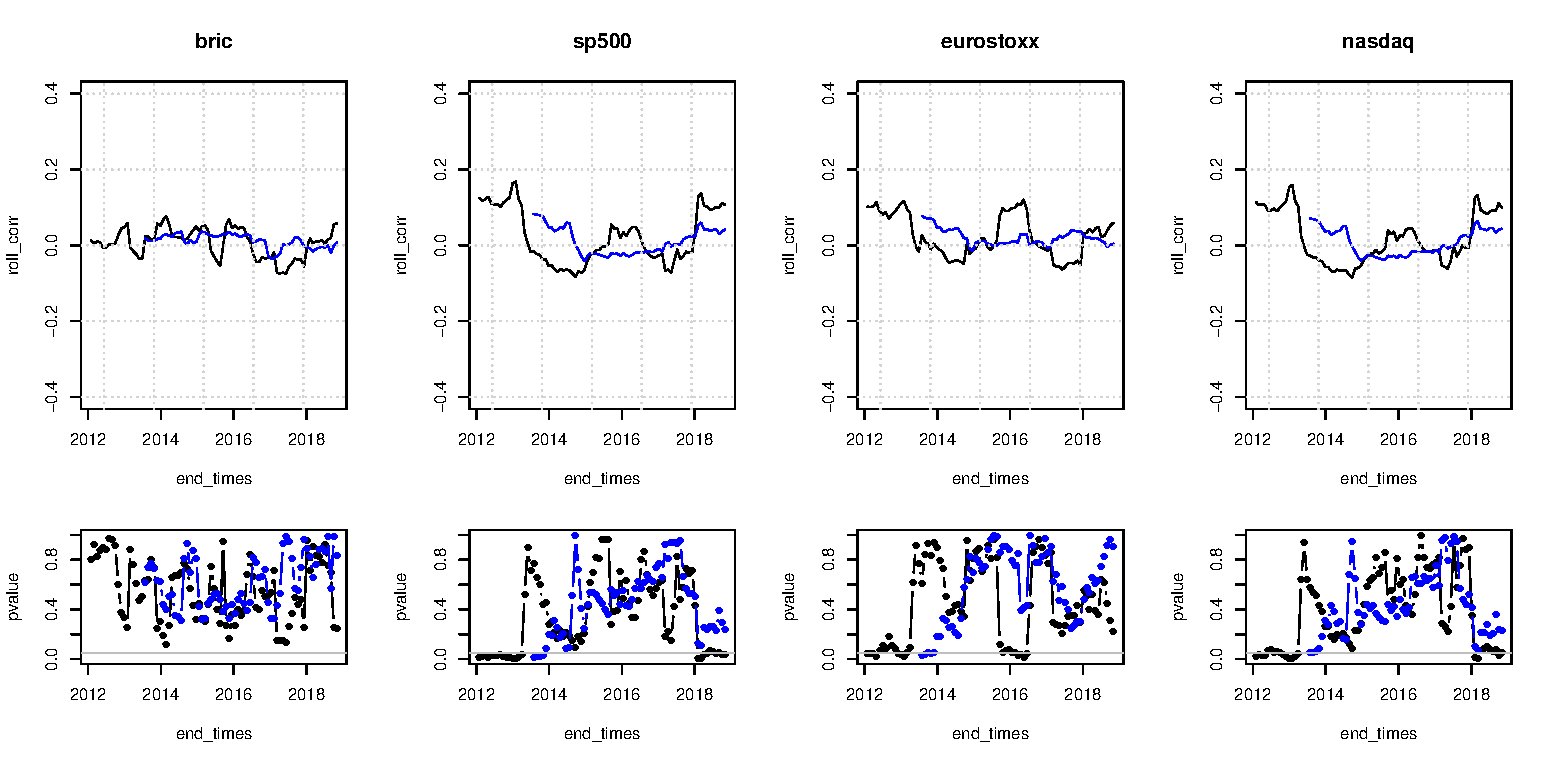
\includegraphics[width=\linewidth]{Images/rolling_stocks}
		\label{roll_stocks}
		\caption{Stocks}
	\end{subfigure}
}
   \noindent\makebox[\textwidth]{
	\begin{subfigure}{0.8\textwidth}
		\centering
		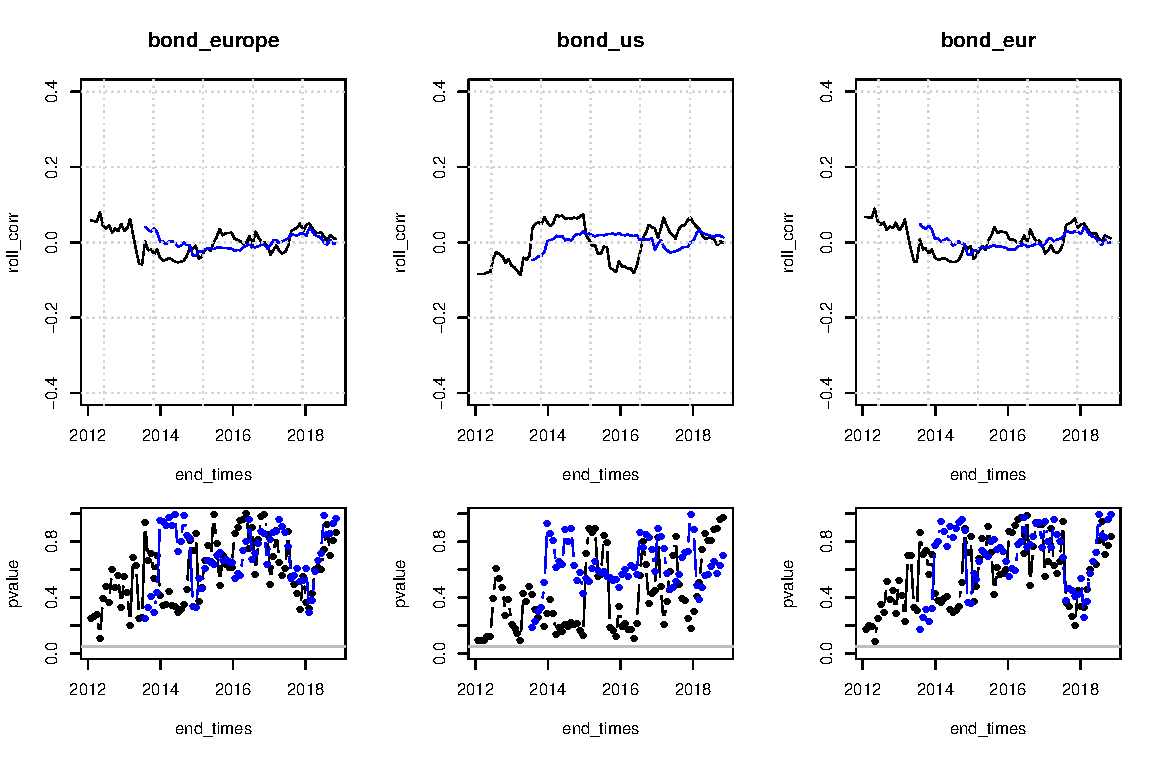
\includegraphics[width=1\linewidth]{Images/rolling_bonds}
		\caption{Bonds}
		\label{roll_bonds}
	\end{subfigure}
}

\caption[Plots of rolling correlations]{Plots of rolling correlation for the different asset classes (on top) and significance for each value (on bottom). Blue lines are the 3-year rolling correlations, while the black ones have a window of 18 months. Both computations are updated monthly.[1/2]}
\label{roll_corr1}
\end{figure}

\begin{figure}
\centering
	\noindent\makebox[\textwidth]{
	\begin{subfigure}{1.2\textwidth}
		\centering
		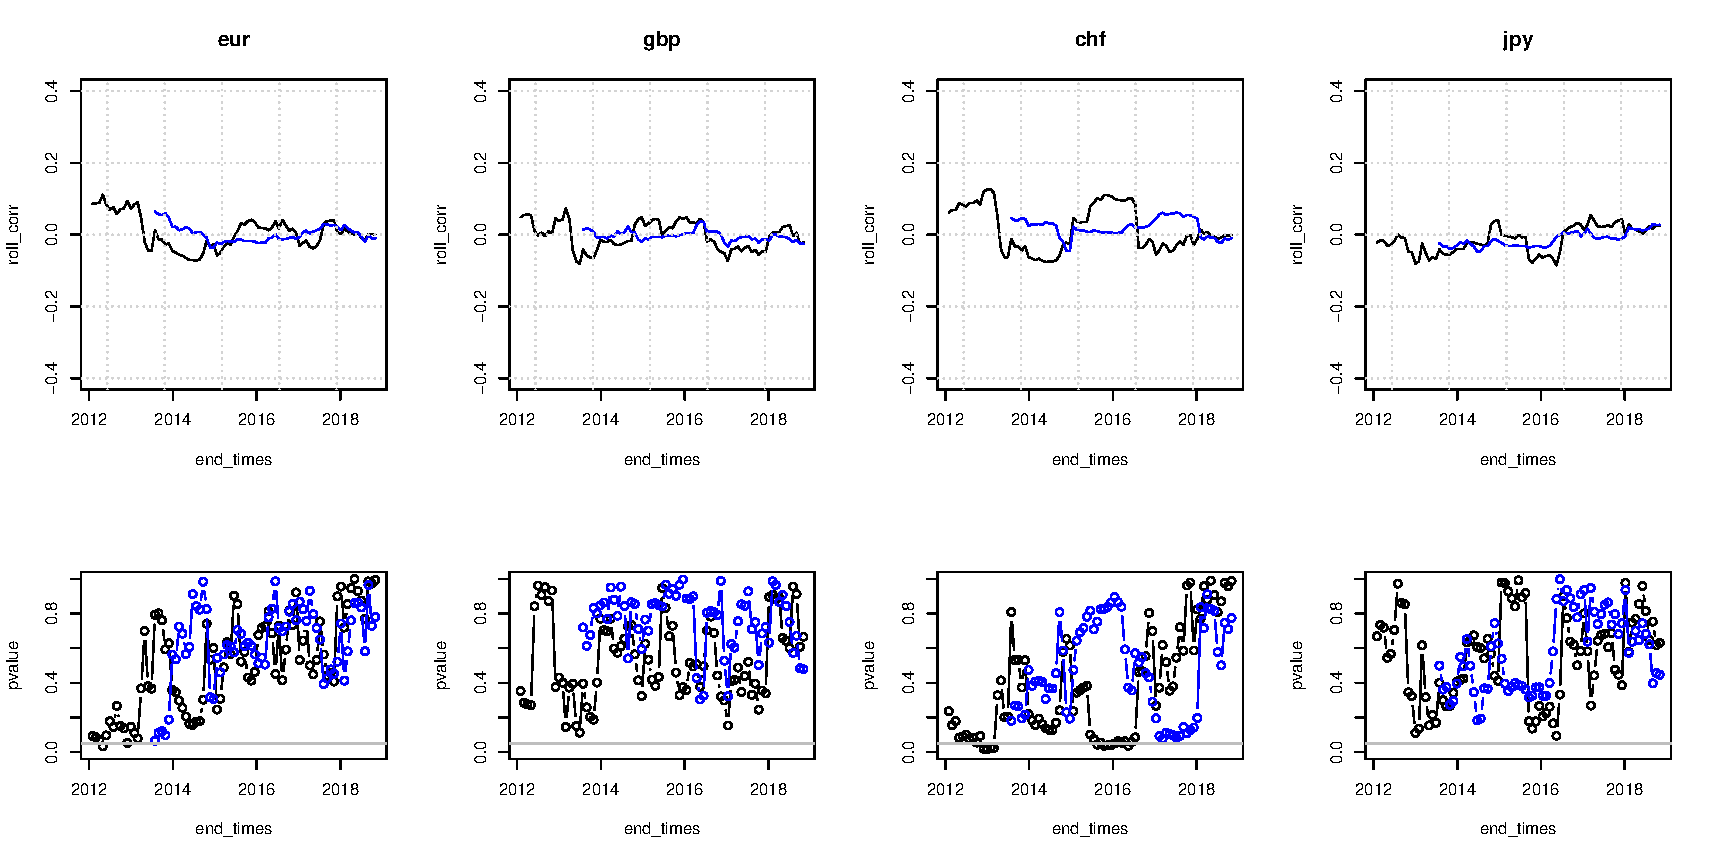
\includegraphics[width=\linewidth]{Images/rolling_fx}
		\caption{Currency exchange}
		\label{roll_currencies}
	\end{subfigure}
}
	\noindent\makebox[\textwidth]{
	\begin{subfigure}{1.2\textwidth}
		\centering
		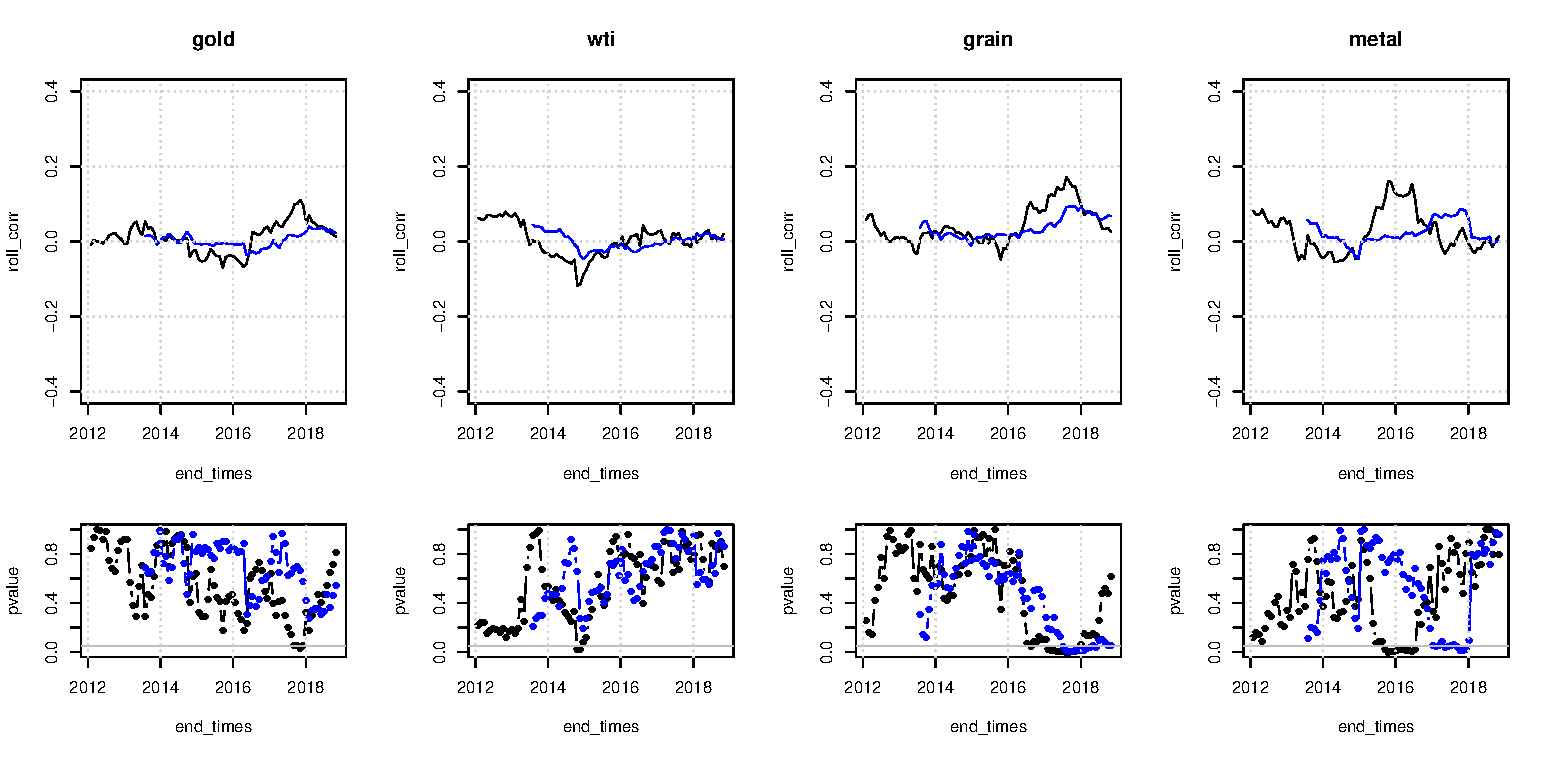
\includegraphics[width=\linewidth]{Images/rolling_commodities}
		\caption{Commodities}
		\label{roll_commodities}
	\end{subfigure}
}
	\caption[Plots of rolling correlations]{Plots of rolling correlation for the different asset classes (on top) and significance for each value (on bottom). Blue lines are the 3-year rolling correlations, while the black ones have a window of 18 months. Both computations are updated monthly.[2/2]}
	\label{roll_corr2}
\end{figure}


There are two graphs for each asset: in the top plots levels of the rolling correlations are represented using two different colours, blue for the 3-year and black for the 18-month windows; in the bottom plots we included the significance of each rolling correlation through its p-value. The grey horizontal line represents the 5\% level of significance\footnote{As we explained in the previous section, to check that a sample correlation is \textit{significantly} non zero, we compare the p-value of the test to a given level, here $1- \alpha$ = 5\%. Graphically, whenever the dots are above the grey line in Figures \ref{roll_corr1} or \ref{roll_corr2}, the corresponding correlation is \textit{not} significantly different from zero.}. 

The main conclusion we can draw from these images is that the correlation of any asset with Bitcoin is hardly ever significantly different from zero, and when it is, its absolute level is never greater than 15\%  unless for a small period of time.

To confirm the fact that Bitcoin is not correlated with any asset, we can also take a look at the path of the rolling correlations: there is no line that is always above zero, nor below. This indicates that there is no underlying trend, whether positive or negative, and the correlation one might happen to find is only temporary.






\chapter{Presentation of the Models}
\label{chpr:models}
In this chapter we will present the stochastic frameworks in which we developed our analysis. We first introduce a \textit{jump diffusion} (JD) model presented in 1976 by R.C. Merton: he added log-normal jumps to the simple B\&S dynamics of the asset price. Then we move to the \textit{stochastic volatility} (SV) model of Heston 1993. Heston introduced a new stochastic process that accounts for the variance of the underlying which evolves as a B\&S  with a stochastic volatility term.
The last model we will present was introduced by Bates in 1996 and it is the combination of the former two: an asset dynamics which include jumps and is driven by a stochastic volatility.
All models are first introduced in the one dimensional case and then generalised to the $n$ dimensional case which was then implemented in our code.

\bigskip

\section{Preliminary Notions}

In this section we will briefly present the equation of a geometric brownian motion, introduce the notion of Poisson process and present the 
CIR process. All of these building blocks will be required to fully understand the models to follow.


\subsection{Geometric Brownian Motion}
The simplest continuous dynamics to describe the price of an asset is that of a geometric brownian motion:
\begin{equation}
	\label{eq:GBM}
	\frac{dS_t}{S_t} = \mu dt + \sigma dW_t
\end{equation}

where $S_t$ represents the price of the asset at time $t$, $\mu$ is the (constant) drift and $\sigma$ is the (constant) volatility. $W_t$ is a Wiener process.
This is the standard and most widespread stichastic differential equation to model asset dynamics, so we will only present those results that will be later used in our study.


Applying Ito's lemma to the previous equation, we can also explicitly express the dynamics of the log-returns $X_t = log(S_t)$ , obtaining:
\begin{equation}
	dX_t = (\mu - 	\frac{\sigma^2}{2}) dt + \sigma dW_t
\end{equation}

This stochastic differential has a simple solution which can be computed via stochastic integrals and allows us to describe the dynamics of the log-returns at each instant $t$ starting from $t=0$:
\begin{equation}
	\label{GBM_ret_sol}
	X_t = X_0 + (\mu - 	\frac{\sigma^2}{2}) t + \sigma W_t
\end{equation}

Thanks to (\ref{GBM_ret_sol}) we can now express the price dynamics of the asset by inverting the relation with the returns: $S_t = e^{X_t}$. 
We thus obtain the solution to (\ref{eq:GBM}):
\begin{equation}
	S_t = S_0 \;e^{(\mu - 	\frac{\sigma^2}{2}) t + \sigma W_t}
\end{equation}

Given that $S_t = e^{X_t}$, that $X_t$ by its equation is a generalized brownian motion and hence we have $X_t - X_0 \sim \mathcal{N}(\mu - 	\frac{\sigma^2}{2}, \sigma^2)$, the resulting distribution of prices at time $t$ as units of the initial value is distibuted as a log-normal.

The great success of these framework comes from the simplicity of its dynamics. In particular, since the log-returns follow a Gaussian distribution, $\mu$ and $\sigma$ are easy to calibrate from data and the formulas for pricing options  are often explicit.
As one can imagine, a simple model can only explain simple phenomena: that's why we have such a great deal of \textit{new and improved} version of equation \ref{eq:GBM}.

\subsection{Poisson Process and Compound Poisson Process}
Consider a sequence of \textit{independent} exponential random variables  $\{\tau_i\}_{i\geq1}$ with parameter $\lambda$\footnote{An exponential random variable $\tau$ of parameter $\lambda$ has a cumulative distibution function of the form: $\mathbb{P}(\tau \geq y) = e^{-\lambda y}$} and let $T_n = \sum_{i=1}^{n}\tau_i$. Then we can define the \textit{Poisson process} $N_t$ as
\begin{equation}
 	N_t = \sum_{n\geq 1} \mathds{1}_{t \geq T_n}
\end{equation}

where $\mathds{1}_{condition}$ is 1 if the \textit{condition} is true, 0 if it is false.

$N_t$ is thus a piece-wise constant RCLL\footnote{RCLL is shorthand for right continuous with left limit.} process with jumps that happen at times $T_n$ and are all of size 1, as we can see from Figure \cref{fig:pois}.
An important property of Posson processes is that they have independent and stationary increments, meaning that the increment of $N_t - N_s$ (with $s\leq t$) is independent from the history of the process up to $N_s$ and has the same law of $N_{t-s}$.
At any time $t$, $N_t$ is distributed as a Poisson of parameter $\lambda t$, which means it is a discrete random variable on the integer set with
\begin{equation}
\label{eq:pois_pdf}
\mathbb{P}( N_t = n) = e^{-\lambda t}\frac{(\lambda t)^n}{n!}
\end{equation}



\begin{figure}
	\centering
	\begin{subfigure}{.5\textwidth}
		\centering
		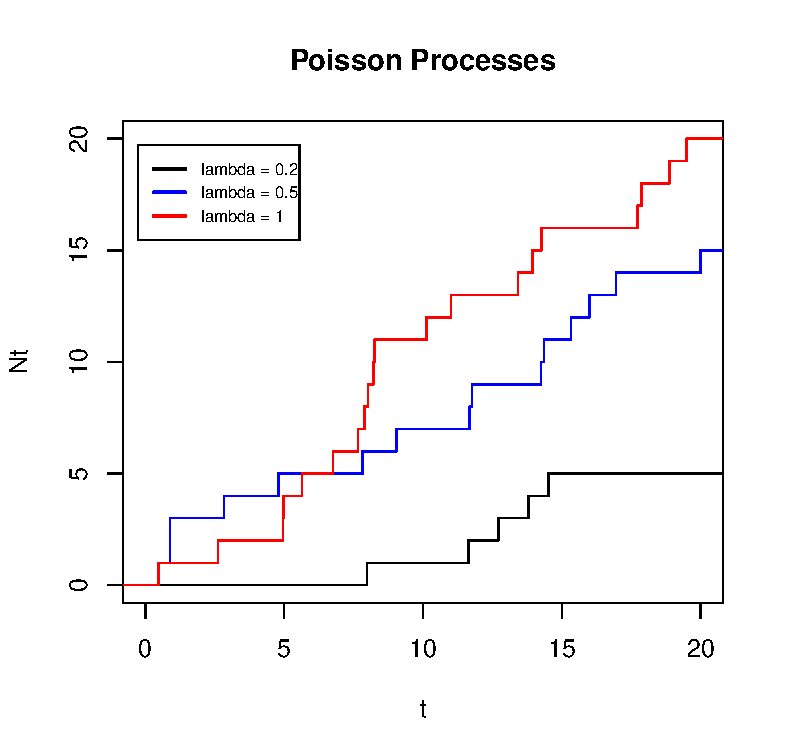
\includegraphics[width=\linewidth]{Images/poisson_process.pdf}
		\caption{Poisson processes.}
		\label{fig:pois}
	\end{subfigure}%
	\begin{subfigure}{.5\textwidth}
		\centering
		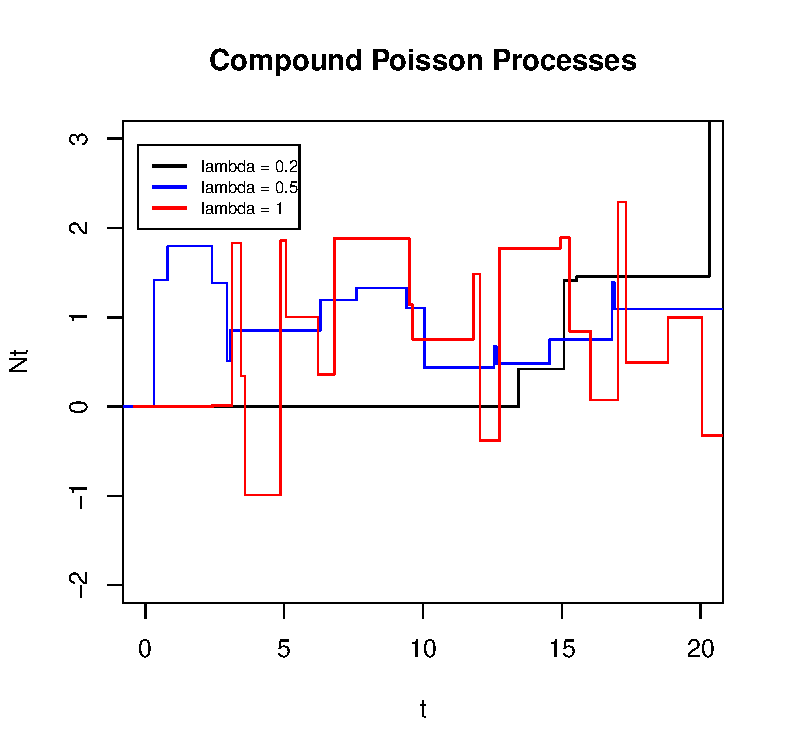
\includegraphics[width=\linewidth]{Images/compound_poisson_process.pdf}
		\caption{Compound with Gaussian jumps.}
		%$\mathcal{N}(1,1)$
		\label{fig:compound_pois}
	\end{subfigure}
	\caption{Poisson processes and compound Poisson processes with different $\lambda$.}
	\label{fig:pois_process}
\end{figure}

When working with jump diffusion process, it is often the case that there is no explicit formula for its density, thus usually we resort to characteristic functions. The characteristic function of $N_t$ is given by 
\begin{equation}
\label{eq:pois_chf}
	\phi_{N_t}(u)=e^{\lambda t (e^{iu}-1)}
\end{equation}

The computations to get \ref{eq:pois_chf} from \ref{eq:pois_pdf} are carried out in Appendix \ref{app:A}. 

\bigskip
For financial applications, it is of little interest to have a process with a single possible jump size. The \textit{compound} Poisson processes are a generalization of Poisson processes  where  the jump sizes can have an arbitrary distribution. More precisely, consider a Poisson process $N_t$ with parameter $\lambda$ and a sequence of i.i.d\footnote{i.i.d stands for independent and identically distributed.} variables ${Y_i}_{i\geq 1}$ with law $f_Y(y)$. Then the process defined by
\begin{equation}
	X_t = \sum_{n=1}^{N_t} Y_i
\end{equation}
is a compound Poisson process. Examples of this kind of process are plotted in Figure \cref{fig:compound_pois}.

As before, we developed the computations to obtain an expression for the characteristic function of $X_t$ in Appendix \ref{app:A}. The resulting expression depends on the distribution of $Y$, specifically from its characteristic function $\phi_Y(u)$:

\begin{equation}
	\phi_{X_t}(u) = e^{\lambda t (\phi_Y(u)-1)}
\end{equation}

Both in Merton's and in the Heston's models there will be a jump component driven by a compound Poisson process with Gaussian jump sizes, as we will see in the following paragraphs.

\subsection{CIR Process}
The CIR process was introduced in \cite{CIR85} in 1985 by Cox, Ingersoll and Ross (hence the name CIR) as a generalization of a Vasicek process to model the mean reverting dynamics of interest rates.
Following their notation, the differential equation for the  evolution of the rate is given by:
\begin{equation}
\label{eq:cir}
	dr_t = \kappa(\theta - r_t) dt + \sigma \sqrt{r_t}dW_t
\end{equation}
where we have three parameters that characterize it: $\theta$ is the \textit{long-term value} of the rate, the asymptotic level which it tends to settle at in the long run;$\kappa$ is the \textit{mean-reversion rate}, the speed at which the rate is pulled back to the $\theta$ value; finally $\sigma$ accounts for the \textit{volatility} of the stochastic component.
When $\kappa,\theta >0$, equation (\ref{eq:cir}) represents a first order mean-reverting auto-regressive process. Moreover, thanks to \textbf{*****add citation*******}, we know that the process will not hit zero if the following condition is satisfied:
\begin{equation}
	2\kappa\theta > \sigma^2
\end{equation}
This condition is usually referred to as \textit{Feller} condition, from the author of the cited paper in which this result was first presented.

An example of a CIR process is shown in Figure (\ref{fig:cir_proc}), where the mean-reverting effect is  clearly visible.

\begin{figure}
	\centering
	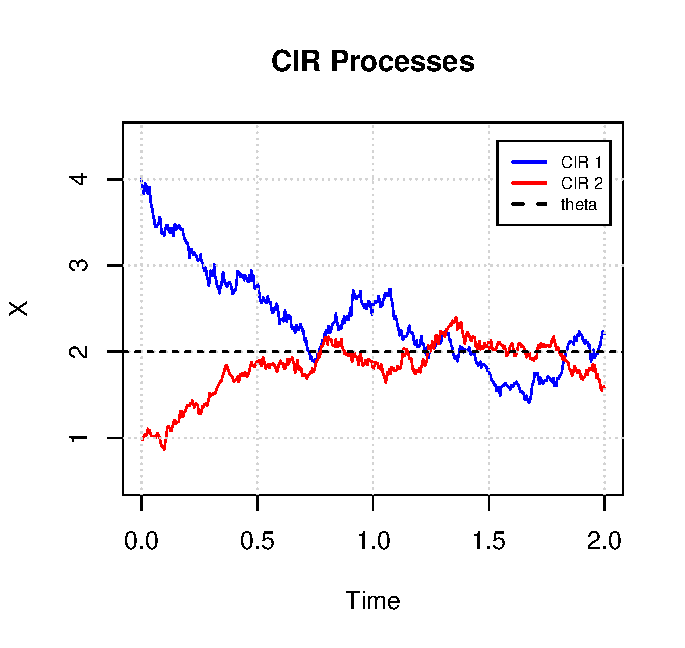
\includegraphics[width=0.6\textwidth]{Images/cir_process.pdf}
	\caption{Two trajectories of the same CIR process: $dr_t = 3(2 - r_t) dt + 0.5 \sqrt{r_t}dW_t$ with different starting point. We can see the mean-reverting effect that attracts both trajectories to the value $\theta=2$. }
	\label{fig:cir_proc}
\end{figure}

When modelling interest rate in continuous time, having $r_t$ hit zero is not an issue since when $r_t=0$ equation (\ref{eq:cir}) reduces to $dr_t = \kappa\theta dt$ which immediately brings the level back to positive values and hence the square root in the dynamics never loses meaning. Conversely, considering a \textit{discretized} version of (\ref{eq:cir}), as is the case in a simulation framework, one needs to pay attention on how he models the increments since a simple Euler discretization scheme may cause $r_t$ to reach \textit{negative} values\footnote{This model was introduced having in mind the certainty that interest rates could never be negative, hence the introduction of a square root in the dynamics. Given recent years interest rates levels, this in no more the case.} and invalidate the whole model representation.

The non negativity of the CIR process will become fundamental when we introduce Heston and Bates SV models, where the (stochastic) variance of the process driving the asset price will be model as a CIR process.

\textcolor{red}{******AGGIUNGERE DISTRIBUZIONE DI rt e di r-inf (gamma)******}

\bigskip
\section{Merton Model}

 ******maybe add some words right here ********
%%% ORIGINAL MODEL
\subsection{Original Univariate Model}
The first jump diffusion model was originally introduced in \cite{MERTON1976} in order to account for the leptokurtic distribution of real market returns and to model sudden falls (or rises) in prices due to the arrival of new information.
The asset price dynamics $S_t$ is modelled as a GBM to which a jump component driven by a compound Poisson process is added:

\begin{equation}
\label{merton_model}
\frac{dS_t}{S_t} = \alpha dt + \sigma dW_t  + (Y_t-1)dN
\end{equation}

where $\alpha$ and $\sigma$ are respectively the drift and the diffusion of the continuous part, $Y_t$ is a process modelling the intensity of the jumps and $N(t)$ is the Poisson process driving the arrival of the jumps and has parameter $\lambda$.

We can rewrite (\ref{merton_model}) in terms of the log-returns $X_t = log(S_t)$ and obtain, following the computations in \cite{MARTIN2007} and using theory from \cite{TANKOV2015}:
\begin{equation}
dX_t = (\alpha - \frac{\sigma^2}{2})dt + \sigma dW_t + \log (Y_t)
\end{equation}

that has as solution:
\begin{equation}
\label{merton_returns}
X_t =X_0 +  \mu t + \sigma W_t + \sum_{k=1}^{N(t)} \eta_k
\end{equation}

where $X_0$ is the initial value of the log-returns, $\eta_k= \log(Y_k) = \log(Y_{t_k})$ and $t_k$ is the time when the $k^{th}$ Poisson shock from $N(t)$ happens. We use $\mu = \alpha - \frac{\sigma^2}{2} $ for ease of notation throughout the paper.
Following \cite{MERTON1976}, we take $\eta_k$ \textit{i.i.d.} (independent and identically distributed) and Gaussian, in particular $\eta \sim \mathcal{N}(\theta, \delta^2)$.
Another choice for the distribution of $\eta$ is given in \cite{KOU2002}. 

%% AGGIUNGERE DENSITA' NEL caso generale [0,T] ?

It is often useful when dealing with market data that are by nature discrete, to consider a \textit{discretized} version of (\ref{merton_returns}) in which the values are sampled at intervals of $\Delta t$ in $[0, T]$. We thus get that for $X_i = \log(\frac{S_{i+1}}{S_i})$:

\begin{equation}
\label{discrete_returns}
X_i =  \mu \Delta t + \sigma \sqrt{\Delta t} \; z +  \sum_{k=1}^{N_{i+1} - N_i} Y_k
\end{equation}

where we denote $X_i = X_{t_i}$, $N_i = N(t_i)$ and $t_i = i \Delta t$ with $i= 0 \dots N$, $t_N = N \Delta t= T$,  $z$ is distributed as a standard Gaussian $ z\sim \mathcal{N}(0,1)$.

The Poisson process $N(t)$ in (\ref{discrete_returns}) is computed at times $t_{i+1}$ and $t_i$ and these quantities are subtracted. Following basic stochastic analysis, one can prove that the resulting value $N_{i+1} - N_i$,  is distributed as a Poisson random variable $N$ of parameter $\lambda \Delta t$.
This allows us to provide an explicit formulation for the transition density of the returns using the theorem of total probability:

\begin{equation}
\label{transitional}
f_{\Delta X} (x) = \sum_{k=0}^{\infty} \mathbb{P}(N = k) f_{\Delta X | N = k}(x) 
\end{equation}

This is an infinite mixture of Gaussian distributions, due to the infinite possible realization of the Poisson variable, and renders the estimation of the model through MLE technique intractable, see \cite{HONORE1998}.
To solve this problem we introduce a first order approximation, as it's been proposed in \cite{BALLTOROUS1983}. Considering small $\Delta t$, so that also $\lambda \Delta t $ is small, we obtain that the only relevant terms in (\ref{transitional}) are the one for $ k = 0, 1$.
The formula for the transition density becomes:
\begin{equation*}
f_{\Delta X} (x) = \mathbb{P}(N = 0) f_{\Delta X | N = 0}(x) + \mathbb{P}(N = 1) f_{\Delta X | N = 1}(x)
\end{equation*}
expressing it explicitly:
\begin{equation}
f_{\Delta X} (x) = (1 - \lambda \Delta t) \;f_{\mathcal{N}}(x ; \mu, \sigma^2) + (\lambda \Delta t)\; f_{\mathcal{N}}(x ; \mu + \theta, \sigma^2+\delta^2)
\end{equation}
where $f_{\mathcal{N}}(x ; \mu, \sigma^2)$ is the density of a Gaussian with parameters $\mathcal{N}(\mu, \sigma^2)$.


%%% MULTIVARIATE MODEL
\subsection{Multivariate Model}
Starting from the univariate model introduced in \cite{MERTON1976}, we developed a generalization to $n$ assets including only idiosyncratic jumps:

\begin{equation}
\frac{dS_t^{(j)}}{S_t^{(j)}} = \alpha_j dt + \sigma_j dW_t^{(j)} + (Y^{(j)}_t -1) dN^{(j)}_t
\end{equation}

where $\mathbf{S}_t$ are the prices of the assets, $j = 1 ... n$ represents the asset, $\alpha_j$ are the drifts, $\sigma_j$ are the diffusion coefficients, $W^{(j)}_t$ are the components of an $n$-dimensional Wiener process $ \mathbf{W}_t$ with $dW^{(j)}dW^{(i)}=\rho_{j,i}$, $\eta_j$ represent the intensities of the jumps and are distributed as Gaussian: $\eta_j \sim \mathcal{N}(\theta_j , \delta_j^2)$. Finally, $N^{(j)}(t)$ are Poisson processes with parameters $\lambda_j$, which are independent of $\mathbf{W}_t$ and of one another. 

In order to calibrate the parameters to the value of the market log-returns, we used a Maximum Likelihood approach. We thus maximize:
\begin{equation}
\mathcal{L}(\psi | \Delta \mathbf{x}_{t_1},\Delta \mathbf{x}_{t_2},\dots,\Delta \mathbf{x}_{t_N}) = \sum_{i=1}^{N} f_{\Delta \mathbf{X}}(\Delta\mathbf{x}_{t_i} | \psi)
\end{equation}

where $\psi = \{ \{\mu_j\},\{\sigma_j\},\{\rho_{i,j}\},\{\theta_j\},\{\delta\}_j,\{\lambda_j\} \}$ are the model parameters, $f_{\Delta \mathbf{X}}$ is the transitional density of the log-returns which is computed approximately using the theorem of total probability.
For a full insight on the model and the calibration procedure, please refer to the *APPENDIX LINK*

\bigskip

\section{Heston Model}

The Heston model was presented in 1993 in \cite{HESTON93} as a new framework to model stochastic volatility in the asset price dynamics, which allows to better fit the skewness and kurtosis of the log-return distribution.

\subsection{Univariate Heston Model}
The Heston model belongs to the family of SD processes, generalizations of B\&S model in which the volatility is no more constant but is itself  stochastic.
\textcolor{red}{***add examples?***}
%Example of SD processes are Heston, CEV, sabr, 3/2 model....

Starting with a GBM as in the B\&S framework, we obtain the dynamics of the price process simply by allowing the volatility in (\ref{eq:GBM}) to evolve over time and specifying how this evolution takes place.
In particular, the dynamics of the \textit{instantaneous} variance $V_t = \sigma_t^2$ for the Heston model is described by a CIR process :
\begin{equation}
	\frac{dS_t}{S_t} = \mu dt +\sqrt{ V_t} dW_t^S
\end{equation}
\begin{equation}
	dV_t = \kappa (\theta - V_t) dt + \sigma_V \sqrt{V_t} dW_t^V
\end{equation}

where $\mu$ represents the drift in the asset prices, $\kappa>0$ and $\theta>0$ are respectively the \textit{mean-reversion} rate  and the long-run level for the $V_t$ process, $\sigma_V>0$ is often referred to as the \textit{volatility of volatility} parameter, in short vol-of-vol.
The two brownian motions $W_t^S$ and $W_t^V$ are correlated with correlation coefficient equal to $\rho$.
The variance process is always strictly positive if the Feller condition $2\kappa\theta > \sigma_V$ is satisfied.

Let us now consider the dynamics of the log-return $x_t = \log (S_t)$, as we did in the Merton case. 
Unfortunately, given the increased complexity of the model due to the SV part, an explicit formula for the density of the log-return is not available and it has to be computed from the Fourier inversion of the characteristic function:
\begin{equation}
\label{eq:chf_inversion}
f_{x_t}(x) = \frac{1}{2\pi}\int_{-\infty}^{+\infty} \phi_{x_t}(i u) e^{i u x} du
\end{equation}

In (\ref{eq:chf_inversion}) we omitted the dependence of $f_{x_t}(x)$ and $\phi_{x_t}(u)$ on model parameters and on the initial values of the log-returns $x_0$ and of the variance process $V_0$. 

\bigskip

To derive the expression of the characteristic function $\phi_{x_t}(u)$, one has to solve a couple of \textit{Fokker-Planck} partial differential equation as is shown in the Appendix of the reference paper by Heston \cite{HESTON93}. This procedure is beyond the scope of this thesis and thus we will only report the final result, which is a log-affine equation on the information at time $t = 0$:

\begin{subequations}
\begin{align}
	\phi_{x_t}(u| x_0, V_0) &= \exp\{A(t,u) + B(t,u) x_0 + C(t,u) V_0\}\nonumber \\
	A(t,u) &= \mu u i t +  \frac{\kappa\theta}{\sigma_V^2} \bigg( (\kappa - \rho\sigma_V u i +d)t - 2 \log\Big[  \frac{1-ge^{dt}}{1-g} \Big] \bigg)\\
	B(t,u) &= i u \\
	C(t,u)&= \frac{\kappa - \rho\sigma_V u i +d}{\sigma_V^2} \:\Big[\frac{1-e^{dt}}{1+ge^{dt}}\Big]
\end{align}
\end{subequations} 
where :
\begin{equation*}
\begin{split}
d&=\sqrt{(\rho \sigma_V u i - \kappa)^2 + \sigma_V^2(u i + u^2)}\\
g&= \frac{\kappa - \rho\sigma_V u i + d}{\kappa - \rho\sigma_V u i - d}
\end{split}
\end{equation*} 



This formulation is the one proposed by Heston in his original paper \cite{HESTON93} but it is shown in \cite{HESTONTRAP}  that it has numerical issues when  pricing Vanilla options using Fourier methods. We will not be pricing any instrument, however we may incur in the same errors when calibrating our model through the techniques explained in Chapter \ref{chpr:calibration}. For this reason, we will be using the alternative formulation presented in \cite{HESTONTRAP}:



%\begin{IEEEeqnarray*}{rCL}
%	\phi_{x_t}(u| x_0, V_0) &=& \exp\{A(t,u) + B(t,u) x_0 + C(t,u) V_0\} \IEEEyesnumber\\
%	A(t,u) &= &\mu u i t +  \frac{\kappa\theta}{\sigma_V^2} \bigg( (\kappa - \rho\sigma_V u i +d)t - 2 \log\Big[  \frac{1-ge^{+dt}}{1-g} \Big] \bigg) \IEEEyessubnumber*\\
%	B(t,u) &= &i u \\
%	C(t,u) &=& \frac{\kappa - \rho\sigma_V u i +d}{\sigma_V^2} \:\Big[\frac{1-ge^{+dt}}{1+g}\Big]\\
%\end{IEEEeqnarray*}

\begin{equation}
% heston trap solution
\begin{split}
\phi_{x_t}^*(u| x_0, V_0) &= \exp\{A(t,u) + B(t,u) x_0 + C(t,u) V_0\}\\
A(t,u) &= \mu u i t +  \frac{\kappa\theta}{\sigma_V^2} \bigg( (\kappa - \rho\sigma_V u i - d)t - 2 \log\Big[  \frac{1-g^*e^{-dt}}{1-g^*} \Big] \bigg)\\
B(t,u) &= i u \\
C(t,u)&= \frac{\kappa - \rho\sigma_V u i - d}{\sigma_V^2} \:\Big[\frac{1-e^{-dt}}{1-g^*e^{-dt}}\Big]
\end{split}
\end{equation} 
where :
\begin{equation*}
\begin{split}
d&=\sqrt{(\rho \sigma_V u i - \kappa)^2 + \sigma_V^2(u i + u^2)}\\
g^*&= \frac{\kappa - \rho\sigma_V u i - d}{\kappa - \rho\sigma_V u i + d} = \frac{1}{g}
\end{split}
\end{equation*} 

The only difference is that the signs of the $d$ terms are all flipped: the origin of the two representations for the characteristic function lies in the fact that the complex root $d$ has two possible values and the second value is exactly minus the first value.
A uniform choice between the two possibilities cannot be made over all the complex plane to obtain a continuous function due to the presence of a branch cut in the graph of $\sqrt{z}$. Selecting the sign of $d$ as in $\phi_{x_t}^*$ and $g^*$ avoids the discontinuity affecting our future computations.

For this reason, from now on we will be using the second formulation while leaving out the star * from our notation.

\bigskip


Our characteristic function still depends on the initial values $x_0$ and  $V_0$ and is thus often called \textit{conditional} characteristic function on $x_0$ and $V_0$.
We can easily remove the dependence on $x_0$ by considering the distribution of incremental returns, namely $\Delta x_t = \log (S_t / S_0) = x_t - x_0$
%, but as for $V_0$, we will need to do some more work.

Applying the definition of characteristic function:
\begin{equation*}
	\begin{split}
	\phi_{\Delta x_t}(u|V_0) &= \mathbb{E}\big[e^{i u \Delta x_t} |V_0\big] \\
	&=  \mathbb{E}\big[e^{i u ( x_t - x_0)}|V_0\big]\\
	&= \mathbb{E}\big[e^{i u x_t}|V_0\big] e^{-i u x_0}\\
	&= \phi_{x_t}(u) e^{-i u x_0}\\
	&= \exp\{A(t,u) + (B(t,u) - iu) x_0 + C(t,u) V_0\}
	\end{split}
\end{equation*}

and since $B(t,u)  = i u$, the second term in the exponential is equal to zero and we are left with:
\begin{equation}
\label{eq:chf_V0}
\phi_{\Delta x_t}(u|V_0) =  \exp\{A(t,u) + C(t,u) V_0\}
\end{equation}




This equation is however still dependent on the initial value of the variance process. In a simulation framework, this would not be an issue, since we can define the level of $V_0$ ourselves and then generate all the different scenarios. However, if we need to calibrate the model parameters from asset prices, the market data for the variance process are not available. We will address more in depth different ways to solve this problem later on in Chapter \ref{chpr:calibration}. As for now, we show that we can obtain an \textit{unconditional} expression for the characteristic function of a Heston process by approximating the distribution of $V_t$ with its stationary distribution.

\begin{equation*}
\begin{split}
	\phi_{\Delta x_t}(u) &= \mathbb{E}\big[e^{i u \Delta x_t} \big] \\
	&= \mathbb{E}\big[ \mathbb{E}\big[ e^{i u \Delta x_t} | V_0\big] \big]\\
	&=  \int_{0}^{\infty} \mathbb{E}\big[e^{i u ( x_t - x_0)}|V_0 = v \big] f_{V_0}(v) dv \\
	&= \int_{0}^{\infty} \exp\{A(t,u) + C(t,u) v\} f_{V_0}(v) dv \\
	&=  \exp\{A(t,u)\} \int_{0}^{\infty}  \exp \{C(t,u) v\} f_{V_0}(v) dv\\
	&= \exp\{A(t,u) \} M_{V_0}(C(t,u))
\end{split}
\end{equation*}

where we have used the Law of Total Expectation and $M_{V_0}(z)$ indicates the \textit{moment generating function} of $V_0$.



\subsection{Parsimonious Multiasset Heston Model}
The problem with generalizing Heston framework to include more than one underlying is that the model becomes quickly very complex: we need 5 parameters for each asset ($\mu, \kappa,\theta, \sigma_V$ and $ \rho$), and we can also model all types of correlation between the different stochastic drivers. In particular, we have 4 types of correlation: 
\begin{itemize}
	\item $ \rho^{S_i , V_i}$:  correlation that we already have in the unidimensional case, that models the way the price and the variance processes are linked ;
	\item $ \rho^{S_i , S_j}$: correlation between the movements in prices of two different assets ;
	\item $\rho^{V_i , V_j} $: correlation between the variance processes of two different assets. One might expect that asset of similar nature have a higher correlation both in the price and in the variance processes;
	\item $\rho^{S_i , V_j} $: correlation between the price process of an asset and the variance process of a different one.
\end{itemize}

To overcome this increase in both mathematical and computation complexity, we will use the \textit{parsimonious} model introduced by Szimayer, Dimitroff and Lorenz in \cite{PARSIMONIOUS2011}. Their framework has two main characteristics: each single-asset sub-model forms a traditional Heston model and the parameters are  composed by $n$ single-asset Heston parameter sets and $n (n-1)/2$  \textit{asset-asset} correlations.

The $n$-dimensional model  hence becomes:

%\begin{equation}
%\frac{dS_i(t)}{S_i(t)} = \mu dt +\sqrt{ V_t} dW_t^S
%\end{equation}
%\begin{equation}
%dV_t = \kappa (\theta - V_t) dt + \sigma_V \sqrt{V_t} dW_t^V
%\end{equation}

 \begin{multline}
\begin{pmatrix}
	dS_i(t) / S_i(t)\\
	dV_i(t)
\end{pmatrix}
= \begin{pmatrix}
\mu_i\\
\kappa_i (\theta_i - V_i(t))
\end{pmatrix}
dt  +\\ \begin{pmatrix}
\sqrt{V_i(t)} & 0 \\
0 & \sigma_{V_i} \sqrt{V_i(t)} 
\end{pmatrix}
\begin{pmatrix}
1 & 0 \\
 \rho_i & \sqrt{1-\rho_i^2} 
\end{pmatrix}
\begin{pmatrix}
dW^{S_i}(t)\\
dW^{V_i }(t)
\end{pmatrix}
\end{multline}

where $dW^{S_i}(t)$ and $dW^{V_i}(t)$ are independent processes and we have written explicitly the dependence between the price and the variance processes.

To fully characterize the model, we need to describe how the different $W^{S_i}$ and $W^{V_i}$ are correlated. In accordance with what was stated earlier, the correlation structure is the following:
\begin{equation}
\label{eq:heston_cor}
\Sigma^{(S,V)} = cor(\boldsymbol{W}^{S}, \boldsymbol{W}^{V}) = \begin{pmatrix}
\Sigma^{S} & 0 \\
0& I_n
\end{pmatrix}
\end{equation}

in which $\Sigma^S = cor(\boldsymbol{W}^{S})$.
Equation (\ref{eq:heston_cor}) mathematically represents what we defined as the correlation structure for our model: we only explicitly define the \textit{asset-asset} correlations through matrix $\Sigma^S$, the dependence of every variance  on other processes is carried over via $\Sigma^S$ and the correlations $\rho_i$.
More clearly, let $(\Sigma^S)_{i,j} = \rho_{i,j}$\footnote{Of course we will have $\rho_{i,j} = 1 $ whenever $i=j$.}:
\begin{itemize}
	\item $dW^{S_i}(t) dW^{S_j}(t) = \rho_{i,j} dt$
	\item $dW^{S_i}(t) dW^{V_j}(t) = \rho_{i,j} \rho_j dt$
	\item $dW^{V_i}(t) dW^{V_j}(t) = \rho_i \rho_{i,j}\rho_j dt $ if $i\neq j$, $dt$ otherwise
\end{itemize}

A detailed representation of a 2-asset \textit{parsimonious} Heston model can be found in the reference paper \cite{PARSIMONIOUS2011}.

%	\begin{bmatrix}
%	ax_{0} + bx_{1} \\           
%	\vdots \\
%	ax_{n-1}+bx_{n}
%	\end{bmatrix} -
%	\begin{bmatrix}
%	z_{1} \\
%	\vdots \\
%	z_{n}
%	\end{bmatrix}
\section{Bates Model}
Bates 


\chapter{Calibration of the Models}
\label{chpr:calibration}

In this chapter we will explain how the different models were calibrated and what difficulties were overcome. Empirical results are included for each section.

\textbf{*****aggiungere commento su diversi tipi di calibrazione e in particolare sul fatto che calibriamo su timeseries*****}
\bigskip

\section{Maximum Likelihood Calibration}
The calibration method that we implemented is the \textit{maximum likelihood} approach, which is a statistical method to obtain the parameters of a target distribution family that best approximate the unknown distribution of the observed data.

Let us call $X = \left\lbrace x_1, x_2, ... , x_N \right\rbrace$ the set of available observations and let $\psi= \left\lbrace \alpha_1, \alpha_2, ... \right\rbrace $ the set of parameters of the distribution $ \mathcal{D}$ that we want to calibrate.
Moreover, define $f_\mathcal{D} (x ; \psi)$ to be the probability density function (pdf) of distribution $\mathcal{D}$ with parameters $\psi$ computed at $x \in \mathbb{D}$, where $\mathbb{D}$ is the domain of the density function.

Our aim is to find the best set of parameters $\psi$ such that we can describe $X$ as samples taken from $\mathcal{D}$:
\begin{equation}
x_i \sim \mathcal{D} (\psi), \: i = 1, \dots, N.
\end{equation}

The estimation of the parameter set $\psi$ can then be obtained by:
\begin{equation}
	\hat{\psi} = \argmax_{\psi \in \Psi} \:\mathcal{L}(\psi |  X),
\end{equation}

where $\mathcal{L}(\psi |  X)$ is the likelihood function for distribution $\mathcal{D}(\psi)$ given the observed data $X$.

In the case that the data in $X$ are i.i.d. we have that the likelihood function can be computed as the product of the probability density function computed at each observation $x_i$:

\begin{equation}
\label{eq:log_likelihood}
\mathcal{L}(\psi |  X) = \prod_{i=1}^{N} f_{ \mathcal{D}}(x_{i}; \psi).
\end{equation}

In practice, it is often common to consider the \textit{log-likelihood} function $\ell(\psi |  X)  = \log \mathcal{L}(\psi |  X)$. The natural logarithm is a monotonic function so the maximum of the log-likelihood function is achieved in the same point as the basic likelihood function.\footnote{By how the likelihood function is defined, it can attain only positive values so that the logarithm of  $\mathcal{L}(\psi |  X)$ is always well defined.}
Taking the logarithm of \eqref{eq:likelihood} also simplifies the expression in that the product now becomes a sum:
\begin{equation}
\label{eq:likelihood}
\ell (\psi |  X) =\mathcal{L}(\psi |  X) = \sum_{i=1}^{N} \log f_{ \mathcal{D}}(x_{i}; \psi).
\end{equation}

The issues that arise from the definition of a maximum likelihood estimator are mainly two.
The first problem is that to use equation \eqref{eq:likelihood} we need to know the pdf of the distribution: this might not always be the case with complicated models that only have an explicit expression for their characteristic function. This is what happens for Heston and Bates model, and, as we will see, we are going to need to invert the chf via Fourier inversion and obtain the pdf numerically.

The second issue is that we need to solve a maximization problem in order to obtain an estimate for the parameters of the distribution: it is well known how optimization routines might perform well for some special circumstance and badly under other, especially when the number of parameters increases. The trade-off is, as usual, between fast computations and robustness of the optimization. To solve this, we will opt for a combination of global and local optimizers.





\section{Calibration of Merton Model}
Let us start by considering how we calibrated the jump diffusion model by Merton. 
We will first present how to obtain the parameters for a single asset model and then move to a multi-asset one.



\subsection{Single Asset Merton Calibration}
As we already introduced, the calibration method that we used is the maximum likelihood approach.

We are going to calibrate the values of the 5 parameters $\psi= \left\{ \mu, \sigma, \mu_J, \sigma_J, \lambda \right\}$ of the jump diffusion model based on the observations of the log-returns $\Delta x_i = \log \frac{S_i}{S_{i-1}}$ for each time interval $\Delta t$. In our analysis, since we are going to use \textit{daily} log-returns, $\Delta t = 1/255$. 

Considering daily log-returns allows us to assume that the different samples of $\Delta x$ are independent and identically distributed according to the distribution of log-returns in Merton model given in \eqref{transitional}.
For ease of reading, we present it again here:
\begin{equation}
\label{eq:merton_full_pdf}
f_{\Delta x } (x; \psi) = \sum_{k=0}^{\infty} \mathbb{P}(N = k) f_{\Delta x | N = k}(x ; \psi) .
\end{equation}

The formula represents an infinite mixture of Gaussian distributions, due to the infinite possible realization of the Poisson variable that accounts for the arrival of jumps. 
This fact has a great downside in terms of maximum likelihood estimation. As discussed in \cite{HONORE1998}, the infinite Gaussian mixture causes the problem of maximizing the (log-)likelihood to be unbounded and thus intractable.

To solve this issue we can introduce a first order approximation, as it has been proposed in \cite{BALLTOROUS1983}. 
Since we are considering a small time interval $\Delta t $, only the first terms of the series in \eqref{eq:merton_full_pdf} become significant. 
In particular, we have that the probabilities to have $k = 0, 1, 2$ jumps in a single time step, as presented in \eqref{eq:pois_pdf}, are:
\begin{subequations}
	\begin{align}
	\mathbb{P}(N = 0) &= e^{-\lambda \Delta t}, \\
	\mathbb{P}(N = 1) &= \lambda \Delta t \: e^{-\lambda \Delta t}, \\
	\mathbb{P}(N = 2) &= \frac{(\lambda \Delta t)^2}{2} \: e^{-\lambda \Delta t}
	\end{align}
\end{subequations}

since $N \sim Pois(\lambda \Delta t)$, which is the Poisson process counting jumps that happen in a $\Delta t$ interval.
Considering $\lambda \Delta t$ as small, we can approximate to the first order  $e^{-\lambda \Delta t} =  1 - \lambda \Delta t +  o((\lambda \Delta t)^2)$. 
We thus obtain that:
\begin{subequations}
	\begin{align}
	\mathbb{P}(N = 0) &= 1-\lambda \Delta t , \\
	\mathbb{P}(N = 1) &= \lambda \Delta t \: (1- \lambda \Delta t) = \lambda \Delta t + o((\lambda \Delta t)^2), \\
	\mathbb{P}(N = 2) &= \frac{(\lambda \Delta t)^2}{2} \: (1-\lambda \Delta t) = o((\lambda \Delta t)^2).
	\end{align}
\end{subequations}


The result is that the only relevant terms in \eqref{eq:merton_full_pdf} are the ones for $ k = 0, 1$.
The formula for the transition density thus  becomes:
\begin{equation}
f_{\Delta x} (x; \psi) = \mathbb{P}(N = 0) f_{\Delta X | N = 0}(x; \psi) + \mathbb{P}(N = 1) f_{\Delta x | N = 1}(x; \psi)
\end{equation}
We can then write this equation explicitly by considering the different distributions of the log-returns in the case of no jumps and a single jump:
\begin{equation}
\label{eq:merton_pdf}
f_{\Delta x} (x; \psi) = (1 - \lambda \Delta t) \;
f_{\mathcal{N}}\Big(x ; \widetilde{\mu}\, \Delta t, \sigma^2 \Delta t\Big) + (\lambda \Delta t)\; f_{\mathcal{N}}(x ; \widetilde{\mu}\, \Delta t + \theta, \sigma^2 \Delta t+\delta^2)
\end{equation}
where $f_{\mathcal{N}}(x ; \mu, \sigma^2)$ indicates the pdf of a Gaussian with parameters $\mathcal{N}(\mu, \sigma^2)$ compute at $x$. We used $\widetilde{\mu} = \mu - \sigma^2/2 -\lambda \mu_J$ as a simpler notation to indicate the drift term in the return dynamics.

The distribution of the sample log-returns is thus given by equation \eqref{eq:merton_pdf} and we can plug it into \eqref{eq:log_likelihood} to obtain the log-likelihood function that we are going to maximize:
\begin{equation}
\label{eq:merton_loglikelihood_single}
	\ell(\psi |  \Delta x) = \sum_{i=1}^{N} \log f_{ \Delta x}(\Delta x_{i}; \psi).
\end{equation}

One can then proceed to maximize equation \eqref{eq:merton_loglikelihood_single} to obtain the optimal parameter set $\psi$:
\begin{equation}
\hat{\psi} = \argmax_{\psi \in \Psi} \:\ell(\psi |  \Delta x)
\end{equation}
\begin{equation}
\Psi = \{ (\mu, \sigma, \mu_J, \sigma_J, \lambda) \in \mathbb{R}^5 \: |\: \sigma,\sigma_J, \lambda >0\}
\end{equation}

\subsection{Multi-asset Merton Calibration}
\label{subsec:multi_merton_cal}

We now know  how to calibrate the Merton parameters when the underlying asset is one.
In the case of multiple assets, we decided to adapt \cite{PARSIMONIOUS2011} both for the model definition and the calibration procedure.
In the referenced paper, the authors present a \textit{parsimonious approach} to the extension of Heston Model to a multi-asset framework. Since this is the approach that we will follow for the multivariate Heston calibration and for Bates as well, we decided to also perform in the same way the calibration of the parameters for Merton.
Using a common approach will allow us to better compare the results, especially in terms of the correlation structure that is what we are ultimately interested in.

The first step in the calibration algorithm is to obtain the parameters of all the single asset models that we are studying. The general way to do this was explained in the previous section. 

The next step involves computing the correlation matrix between the different Brownian motions that drive each single-asset model. 
The way this computation is carried out in \cite{PARSIMONIOUS2011} is by asset pairs: we consider each possible couple of assets and try to obtain the model correlation that best approximates the observed correlation.
Let us see how this is achieved more in detail in the case of only two assets.

The problem we are trying to solve is, given the observed sample correlation $\rho_{obs}$ between two assets' returns, find the best model correlation $\rho_{model}$ that solves $\bar{\rho}(\rho_{model}) = \rho_{obs}$.
$\bar{\rho}$ is the expectation of the correlation that we find when computing the  empirical correlation of the returns simulated using $\rho_{model}$.

More precisely, we have to simulate $N_{sim}$ different realisations of the 2-asset model in a given time period $[0, T]$ with the same $\Delta t$ that we have in the observed data, using $\rho_{model}$ as the correlation between the two driving Brownian motions. We then proceed to compute the correlation of the simulated log-returns $\rho_{scen}$ in each scenario and then we take the average of this values. What we obtain is $\bar{\rho} = \mathbb{E}[\rho_{scen}] $.

In order to simulate a two-asset Merton model, we used the following discretization for the log-returns:
\begin{subequations}
	\label{eq:merton_discretization}
	\begin{align}
	x_i^{(1)} &= x_{i-1}^{(1)} + (\mu_1 - \sigma_1^2/2 -\lambda_1 {\mu_J}_1) \Delta t + \sigma_1 \sqrt{\Delta t} \;  z_1 + N_1 {y}_1 ,\\
	x_i^{(2)} &= x_{i-1}^{(2)} + (\mu_2 - \sigma_2^2/2 -\lambda_2 {\mu_J}_2) \Delta t + \sigma_2 \sqrt{\Delta t} \; z_2 + N_2 {y}_2 ,
	\end{align}
\end{subequations} 
where:
\begin{itemize}
	\item $i = 1, \dots , N_{step}$ represents the i-th time-step in our simulation: $x_i = x_{t_i}$ and $N_{step} = T / \Delta t$ so that $t_i = i \Delta t$. The value of the initial return $x_{t_0}$ does not affects the final correlation so we can simply set it to zero.
	\item $z_1$ and $z_2$ are the first and second component of a Gaussian vector $\mathbf{z} = (z_1,z_2)^T$ that is distributed as $\mathbf{z} \sim \mathcal{N}_2(\mathbf{0}, Corr)$. $Corr$ is the $2 \times 2$ matrix composed of ones in the main diagonal and $\rho_{model}$ in the remaining two spots. 
	More simply, $\mathbf{z}$ is a two dimensional Gaussian with zero mean with covariance matrix equal to the correlation matrix of the model.
	\item $N_1$ and $N_2$ are in general the realizations of two Poisson random variables with parameters $\lambda_1 \Delta t$ and $\lambda_2 \Delta t$ respectively. Given our first order approximation in the density and considering small $\Delta t$,  $N_1$ and $N_2$ are actually two Bernoulli with probability of success (i.e. a jump happens) equal to $\lambda_1 \Delta t$ and $\lambda_2 \Delta t$.
	\item Finally, $y_1$ and $y_2$ are the jump intensities and are realisations of Gaussian variables with parameters $\mathcal{N}({\mu_J}_1, {\sigma_J}_1^2)$ and $\mathcal{N}({\mu_J}_1, {\sigma_J}_1^2)$ . 
\end{itemize}

Through \eqref{eq:merton_discretization} we can thus simulate $ x_i^{(1,k)}$ and 
$ x_i^{(2,k)}$ for $k= 1, ... ,N_{sim}$  and compute for each scenario the correlation observed from the simulated returns $\rho_{scen}^{(k)} = corr(x_i^{(1,k)}, x_i^{(2,k)})$.
From these values we can easily compute $\bar{\rho}$:
\begin{equation}
\label{eq:expected_model_correlation}
	\bar{\rho} = \mathbb{E} [\rho_{scen}] = \frac{1 }{N_{sim}} \sum_{k=1}^{N_{sim}} \rho_{scen}^{(k)}
\end{equation}


We have that implicitly the value of the \textit{expected model correlation} $\bar{\rho}$ is a function of the model correlation $\rho_{model}$. The equation we need to solve is then represented by:
\begin{equation}
\label{eq:expected_observed}
\bar{\rho}(\rho_{model}) = \rho_{obs},
\end{equation}

as we have already stated earlier in this section.

\bigskip
In the case of an $n$-asset model, we have to repeat the previous passages for all possible $n(n-1)/2 $ different pairs of assets. We then can build a $n \times n$ matrix $M$ that has ones in the main diagonal and in each element $(l,m), l \neq m$ stores the corresponding model correlation $\rho_{model}^{(l,m)}$.
This matrix may not be a well defined correlation matrix: it may happen that $M$ is not positive definite.
The last step to obtain a proper correlation matrix for our $n$-asset model is to perform some form of \textit{regularization} on $M$ that transforms it into a well defined correlation matrix: positive definite, with elements in the range $[-1,1]$ and ones in the main diagonal.

Through empirical study performed in the reference paper \cite{PARSIMONIOUS2011}, it turns out the best algorithm between the one proposed by the authors is the regularization by J\"ackel, that we briefly present here.

\bigskip
\textbf{Regularization algorithm by J\"ackel:}
\begin{enumerate}
	\item[\textbf{Input}] Model correlation matrix $M$ (not necessarily positive definite).
	\item Perform an eigenvalue decomposition on $M  = S \Lambda S^T$, where $\Lambda = diag(\lambda_l)$ and $\lambda_l$ are the eigenvalues of matrix $M$.
	\item Define $\Lambda^{'} = diag(\lambda_l^{'}$ with $\lambda_l^{'} = \max(\lambda_l, 0))$ as the diagonal matrix that contains the positive part of each eigenvalue.
	\item Create the diagonal matrix $T = diag(t_l)$ where $t_l =1 / \sum_{m} (S_{l,m})^2 \lambda_l^{'}$ .
	\item Define $B = \sqrt{T} S \sqrt{\Lambda^{'}}$.
	\item Set $\widehat{M} = B B^T$.
	\item[\textbf{Output}] Positive definite correlation matrix $\widehat{M}$.
\end{enumerate}

Hence, $\widehat{M}$ is the model correlation matrix that best represents the observed correlation values and that forms the structure of dependence between the Brownian motions that drive each asset in a multivariate Merton model.

\section{Calibration of Heston Model}
Calibrating the Heston model on time-series data presents an added difficulty since we only have data on the price process, while the model also takes into consideration the dynamics of the variance as a stochastic process. 

The problem of deducing the parameter of a \textit{non-observable} process from the observable states of a system is called \textit{filtering} and is in general a complicated numerical procedure. There are nonetheless a few studies in the literature on the subject of calibrating the Heston model through filtering. \textbf{***ADD REFERENCE***}

In our analysis we preferred to keep the same approach to the calibration for all the three models. We will thus proceed to explain how we can perform a maximum likelihood calibration in the case of stochastic volatility and, in the next section, of both jumps and stochastic volatility.

\subsection{Single Asset Heston Calibration}
The first issue that we have to overcome is that an explicit formula for the probability density function of the log-returns is not available and we have to resort to performing a Fourier inversion on the characteristic function, as we already showed in equation \eqref{eq:chf_inversion}

This allows us to have a pdf for the log-return $x_t = \log S_t $ but in order to be able to perform a maximum likelihood calibration in the same way that we did in the  previous section, we need to have the distribution for $\Delta x_t = \log (S_{t + \Delta t} / S_t)$ and make sure that they are i.i.d. so that we can apply \eqref{eq:log_likelihood}.

In order to obtain the pdf for the incremental log-returns $\Delta x_t$, we first need the distribution of  $\Delta x_{[0, t] }= \log (S_t / S_0)$ we can simply proceed as we explained in Chapter \ref{chpr:models} in the section about Heston model to get the characteristic function for $\Delta x_{[0, t] }$ conditioned on the values of $V_0$: 

\begin{equation}
\phi_{\Delta x_{[0, t] }}(u|V_0) =  \exp\{A(t,u) + C(t,u) V_0\}.
\end{equation}

The full expressions for $A(t,u)$ and $C(t,u)$ are given in \eqref{eq:heston_chf+ABC}.
Notice that we omitted the dependence on the model parameters $\psi = \{\mu, \kappa, \theta, \sigma_V, \rho \}$ for ease of notation.

\bigskip
We are now left with the distribution of $\Delta x_{[0, t] }$ as a function of $V_0$: this represents an issue since moving from $\Delta x_{[0, t] }$ to $\Delta x_t  = \Delta x_{[t, t + \Delta t]}$ we have a dependence on the value of $V_t$ which is not available. Moreover, even if data for $V_t$ was indeed available, considering different time-steps $t_i$ for $\Delta x_{t}$, the data samples of $\Delta x_{t_i}$ would not be identically distributed as they depend on levels of the variance $V_{t_i}$ which are different.

Hence the need for an \textit{unconditional} characteristic function to get rid of the dependence on initial variance. We followed the approach that was introduced in \cite{DRAGULESCU2002} of integrating out the dependence on $V_0$. The computations to obtain it were presented in Chapter \ref{chpr:models}.
The unconditional chf for the Heston model has the following expression:
\begin{equation}
 \phi_{\Delta x_t}(u) = \exp\{A(\Delta t,u) \} M_{\Gamma}(C(\Delta t,u))
\end{equation}


with $M_{\Gamma}$ as the moment generating function of a Gamma distribution:
\begin{subequations}
\begin{align}
	M_{\Gamma} (z) &= \Big(\frac{\omega}{\omega-z}\Big)^\nu \nonumber \\
	\omega&= \frac{2\kappa}{\sigma_V^2} \nonumber\\
	\nu&= \frac{2\kappa\theta}{\sigma_V^2}\nonumber
\end{align}
\end{subequations}

We now have a specific expression for the unconditional characteristic function of $\Delta x_t$ and we can obtain the corresponding density by Fourier inversion:

\begin{equation}
\label{eq:uncond_inversion}
f_{\Delta x_t}(x) = \frac{1}{2\pi}\int_{-\infty}^{+\infty}  \phi_{\Delta x_t}(i u) e^{i u x} du
\end{equation}


Another advantage of using the uncoditional chf is that since all the observed log-returns $\Delta x_i = \Delta x_{t_i} $ are considered to be sampled from the same distribution, we can numerically perform the inversion in \eqref{eq:uncond_inversion} using the Fast Fourier Transform (FFT). This allows for a great increase in the speed of the numerical computations since we can obtain the value of the pdf for all different $\Delta x_i$ with a single inversion.
The main ideas behind the FFT algorithm are explained in Appendix \ref{app:FFT}.


Now that we have the density function of $\Delta x$ with parameters $\psi = \{\mu, \kappa, \theta, \sigma_V, \rho \}$ we are able to compute the log-likelihood function by substituting \eqref{eq:uncond_inversion} in \eqref{eq:likelihood}.


In order to perform the maximization of the log-lokelihood function to calibrate the parameters, we have to make sure that the Feller condition \eqref{eq:feller_condition} is satisfied.

The MLE procedure will thus need to be performed including an additional constraint in the optimization given by Feller condition:
\begin{equation}
\widehat{\psi} = \argmax_{\psi \in \Psi} \:\ell(\psi |  \Delta x)
\end{equation}
\begin{equation}
	\Psi = \{ (\mu, \kappa, \theta, \sigma_V, \rho) \in \mathbb{R}^5 \: |\: \kappa,\theta,\sigma_V >0, \rho \in [-1,1], 2\kappa\theta \geq \sigma_V \}
\end{equation}

\subsection{Multi-asset Heston Calibration}
\label{sec:multi_heston_cal}
As we already stated in this paper, the approach to extending the Heston model to $N$ assets that we are taking into consideration is the parsimonious multi-asset model introduced by Dimitroff et al. in \cite{PARSIMONIOUS2011}.
It's called \textit{parsimonious} since, as we explained in chapter \ref{chpr:models}, we are only modelling the asset-asset correlations.

The procedure to calibrating a $N$ asset model is the same that we presented in the multi-asset Merton section and consists of three parts.

Firstly, we have to calibrate all the single asset parameters by themselves. Then we can proceed to compute each asset-asset correlation by solving \eqref{eq:expected_observed} through the simulation of the realization of the log-returns in different scenarios.
Finally, we perform J\"ackel regularization algorithm to make that the final output matrix is indeed a correlation matrix.

The main steps were all presented in section \ref{subsec:multi_merton_cal}, here we will only give the details for the simulation of a two-asset Heston model.

Since we now have two processes for each asset, we have to simulate the path for both, in each time-step.
The discretized dynamics of the log-returns and the variance for a single asset are the following:

\begin{subequations}
	\label{eq:discrete_heston}
	\begin{align}
		x_i &= x_{i-1} + (\mu -  \frac{V_{i-1}}{2})\Delta t + \sqrt{V_{i-1} \Delta t} \:z_x, \\
		V_i &= V_{i-1} + \kappa(\theta - V_{i-1} )\Delta t + \sigma_V \sqrt{V_{i-1} \Delta t} \: z_V
	\end{align}
\end{subequations}
with $z_x$ and $z_V$ that are the two components of a Gaussian vector with mean zero and correlation $\rho$\footnote{In a more extensive form: $ \mathbf{z} = \begin{pmatrix}
	z_x\\ z_V
	\end{pmatrix} \sim \mathcal{N}_2 \Big(\begin{pmatrix}
	0\\ 0\end{pmatrix}, \begin{pmatrix}
	1& \rho\\ \rho&1
	\end{pmatrix} \Big)$}. 

The issue that arises when moving from a continuous dynamics to a discrete one as in \eqref{eq:discrete_heston} is that the variance $V_i$ might assume negative values even if the Feller condition is verified. This happens because the second and third term in the equation of the variance process may be so negative that combined with the first term $V_{i-1}$ the result is less than zero.
Having $V_i < 0$ causes the next update at $i+1$ to be undefined since we would have to compute the square root of a negative value in a real framework.

To solve this issue, a number of possible solutions have been proposed and are collected in \cite{LORD2010}. Among those we have:
\textit{absorption}, which consists in setting $V_i = 0$ when it is negative, \textit{reflection}, taking the absolute value $V_i = |V_i|$, and finally \textit{full truncation}, which is the solution proposed in \cite{LORD2010} and the one we will implement. It is obtained modifying \eqref{eq:discrete_heston} as following:

\begin{subequations}
	\label{eq:full_truncation}
	\begin{align}
	x_i &= x_{i-1} + (\mu -  \frac{V_{i-1}^+}{2})\Delta t + \sqrt{V_{i-1}^+ \Delta t} \:z_x, \\
	V_i &= V_{i-1} + \kappa(\theta - V_{i-1}^+ )\Delta t + \sigma_V \sqrt{V_{i-1}^+ \Delta t} \: z_V.
	\end{align}
\end{subequations}
The notation $y^+ = \max(y, 0)$ indicates the positive part of $y$. 

Equations \eqref{eq:full_truncation} represent the single asset simulation scheme but in order to calibrate the asset-asset correlations as already stated we need to simulate the time-series for a pair of assets.

The updating computations only amount to repeating the single scheme twice:
\begin{subequations}
	\label{eq:full_truncation2}
	\begin{align}
	x_i^{(1)} &= x_{i-1}^{(1)} + (\mu_1 -  \frac{\Big(V_{i-1}^{(1)}\Big)^+}{2})\Delta t + \sqrt{\Big(V_{i-1}^{(1)}\Big)^+ \Delta t} \:z_{x^{(1)}}, \\
	V_i^{(1)} &= V_{i-1}^{(1)} + \kappa_1(\theta_1 - \Big(V_{i-1}^{(1)}\Big)^+ )\Delta t + \sigma_{V^{(1)}} \sqrt{\Big(V_{i-1}^{(1)}\Big)^+ \Delta t} \: z_{V^(1)},\\
	x_i^{(2)} &= x_{i-1}^{(2)} + (\mu_2 -  \frac{\Big(V_{i-1}^{(2)}\Big)^+}{2})\Delta t + \sqrt{\Big(V_{i-1}^{(2)}\Big)^+\Delta t} \:z_{x^{(2)}}, \\
	V_i^{(2)} &= V_{i-1}^{(2)} + \kappa_2(\theta_2 - \Big(V_{i-1}^{(2)}\Big)^+ )\Delta t + \sigma_{V^{(2)}} \sqrt{\Big(V_{i-1}^{(2)}\Big)^+ \Delta t} \: z_{V^{(2)}}.
	\end{align}
\end{subequations}

The important difference with the single asset case is the correlation structure. In order to simulate the random vector $\mathbf{z} = (z_{x^{(1)}}, z_{V^{(1)}}, z_{x^{(2)}}, z_{V^{(2)}})^T$ we have to extract it from a 4-dimensional Gaussian with zero mean and covariance given by $\Sigma$ where:
\begin{equation}
\label{eq:corr_matrix}
	\Sigma = \begin{pmatrix}
	1 	& \rho_1 & \rho_{1,2} & \rho_{1,2} \rho_2\\
	\rho_1 & 1 & \rho_1 \rho_{1,2} & \rho_1 \rho_{1,2} \rho_2\\
	 \rho_{1,2} & \rho_1 \rho_{1,2}  & 1 & \rho_2 \\
	 \rho_{1,2} \rho_2 & \rho_1 \rho_{1,2} \rho_2&\rho_2  & 1
	\end{pmatrix}
\end{equation}

We could also use the Cholesky decomposition of $\Sigma = L L^T$ in order to obtain $\mathbf{z} = L \mathbf{\tilde{z}}$ from a standard 4-dimensional Gaussian vector\footnote{The standard Gaussian vector of dimension $n$ is a normal random vector with mean vector zero and the identity matrix as covariance matrix: $\mathcal{N}_n (\mathbf{0}, \mathbf{I}_n)$. This means that all the components are independent from one another.} $\mathbf{\tilde{z}}$. In this case matrix $L$ would be lower triangular and defined as:
\begin{equation}
	L = \begin{pmatrix}
	1&0&0&0\\
	\rho_1 & \sqrt{1- \rho_1^2} &0&0\\
	\rho_{1,2} &0&\sqrt{1-\rho_{1,2}^2}&0\\
	\rho_{1,2}\rho_2 & 0& \rho_2 \sqrt{1-\rho_{1,2}^2}&\sqrt{1- \rho_2^2} 
	\end{pmatrix}.
\end{equation}

From here on, the procedure is the same as for Merton:
we need to solve \eqref{eq:expected_observed} for every possible asset pair to obtain the model correlation M.

The final step is to apply  J\"ackel regularization algorithm to obtain a valid correlation matrix $\widehat{M}$.

\section{Calibration of Bates Model}
The algorithm to compute the value for the parameters of the Bates model is the same as the two previous ones, so in the following sections we will only focus on the main differences in the functions and equations.

\subsection{Single Asset Bates Calibration}
As it was the case for the Heston model, there is no explicit formula for the density of the log-returns $\Delta x_t$. Moreover, the characteristic function is dependent on the initial value of the variance process, unless we use the approximation that we presented in Chapter \ref{chpr:models} to obtain \eqref{eq:bates_uncond_chf}.

We can then go ahead and compute the corresponding density function by Fourier inversion: we can perform this computation using the FFT algorithm that allows for an increase in the performance speed. 
Arguing in the same way as in previous sections, having the pdf of $\Delta x$ we can compute it for all the observations of $\Delta x_i$ with a single inversion.

Finally, to calibrate the model we need to perform the maximization of the log-likelihood function, making sure the parameters satisfy the Feller condition:

\begin{equation}
\widehat{\psi} = \argmax_{\psi \in \Psi} \:\ell(\psi |  \Delta x)
\end{equation}
\begin{multline}
\Psi = \{ (\mu, \kappa, \theta, \sigma_V, \rho, \mu_J, \sigma_J, \lambda) \in \mathbb{R}^8 \: |\: \\
\kappa,\theta,\sigma_V,\sigma_J, \lambda >0, \rho \in [-1,1], 2\kappa\theta \geq \sigma_V \}
\end{multline}

\subsection{Multi-asset Bates Calibration}
Again, the generalization to the multivariate case we present is an adaptation from \cite{PARSIMONIOUS2011}. The model is be the same as the one in section \ref{sec:multi_heston_cal} with the addition of the jump component.

The calibration algorithm is composed of the three parts concerning the calibration of all the single asset models, computing the asset-asset correlations by simulating the processes, and regularizing the model correlation matrix in order to obtain an acceptable correlation matrix, with ones in the main diagonal, all other elements in the $[-1,1]$ range and that is positive definite.

The simulation for a single asset is performed through the following scheme, implementing the \textit{full truncation} approach to solving the issue with the variance being negative:

\begin{subequations}
	\label{eq:bates_sim}
	\begin{align}
	x_i &= x_{i-1} + (\mu -  \frac{V_{i-1}^+}{2}- \lambda \mu_J)\Delta t + \sqrt{V_{i-1}^+ \Delta t} \:z_x + N y, \\
	V_i &= V_{i-1} + \kappa(\theta - V_{i-1}^+ )\Delta t + \sigma_V \sqrt{V_{i-1}^+ \Delta t} \: z_V,
	\end{align}
\end{subequations}

where $y$ is the jump intensity and is distributed as a Gaussian $\mathcal{N}(\mu_J, \sigma_J^2)$ and $N$ is the Poisson variable with parameter $\lambda \Delta t$ which, given our approximation for small $\Delta t$, is equivalent to a Bernoulli with probability of success equal to $\lambda \Delta t$. 
$z_x$ and $z_V$ are the two components of a Gaussian vector with mean zero and correlation $\rho$.

The same scheme applied to a  2-asset model is the following:
\begin{subequations}
	\label{eq:bates_full_truncation2}
	\begin{align}
	x_i^{(1)} &= x_{i-1}^{(1)} + (\mu_1 -  \frac{\Big(V_{i-1}^{(1)}\Big)^+}{2} \lambda_1\mu_{J_1})\Delta t + \sqrt{\Big(V_{i-1}^{(1)}\Big)^+ \Delta t} \:z_{x^{(1)}} + N_1 y_1, \\
	V_i^{(1)} &= V_{i-1}^{(1)} + \kappa_1(\theta_1 - \Big(V_{i-1}^{(1)}\Big)^+ )\Delta t + \sigma_{V^{(1)}} \sqrt{\Big(V_{i-1}^{(1)}\Big)^+ \Delta t} \: z_{V^(1)},\\
	x_i^{(2)} &= x_{i-1}^{(2)} + (\mu_2 -  \frac{\Big(V_{i-1}^{(2)}\Big)^+}{2} \lambda_2 \mu_{J_2})\Delta t + \sqrt{\Big(V_{i-1}^{(2)}\Big)^+\Delta t} \:z_{x^{(2)}} + N_2 y_2, \\
	V_i^{(2)} &= V_{i-1}^{(2)} + \kappa_2(\theta_2 - \Big(V_{i-1}^{(2)}\Big)^+ )\Delta t + \sigma_{V^{(2)}} \sqrt{\Big(V_{i-1}^{(2)}\Big)^+ \Delta t} \: z_{V^{(2)}},
	\end{align}
\end{subequations}
where the parameters and variables have the same meaning as in the single asset framework.
The random vector $\mathbf{z} = (z_{x^{(1)}}, z_{V^{(1)}}, z_{x^{(2)}}, z_{V^{(2)}})^T$ is a 4-dimensional Gaussian with zero mean and covariance $\Sigma$ expressed in \eqref{eq:corr_matrix}. We can also consider the Cholesky decomposition $\Sigma= L L^T$ to sample the vector $\mathbf{z}$ from the independent Gaussian vector $\mathbf{\tilde{z}}$ by doing $\mathbf{z} = L \mathbf{\tilde{z}}$.

After we have calibrate each asset-asset correlation by solving \eqref{eq:expected_observed}, we need to perform J\"ackel regularization algorithm to obtain a valid model correlation matrix.

\section{Empirical results}
We will now present the specifics of how the calibration procedure was implemented in our study, including the numerical results that it yielded.
All the code to perform the computations was developed in R for greater portability across platforms.

\subsection{Merton Calibration Results}
One of the core aims of this study is to compare the values of the empirical correlation of Bitcoin with other main assets as presented in Chapter \ref{chpr:corr_analysis} with the same correlations computed using more sophisticated models, in our case Merton, Heston and Bates.

The calibration algorithm to compute the parameters of the Merton model was implemented step by step as presented in the previous sections.

In order to perform the single-asset calibration we need to specify the boundaries for the domain of the parameter set $\psi =  \left\{ \mu, \sigma, \mu_J, \sigma_J, \lambda \right\}$ and which optimizer we are going to use.
In our analysis, the optimization is carried out by first taking advantage of a global optimizer and then performing a local maximization\footnote{Since most optimization packages implemented in R usually perform minimization as default, we coded the minimization of the \textit{negative} log-likelihood instead of the maximization of the (positive) log-lkelihood.}

The global optimizer we adopted is implemented in the R package \texttt{DEoptim} and performs \textit{Differential Evolution} optimization: the DE algorithm starts with a population of points randomly sampled from the search space and at each iterations creates new candidate solutions and only keeps the one that best improve the objective function. More information on the package can be found in \cite{DEoptim_manual} and an example of its usage in calibrating a JD process in \cite{DEoptim_jumpdiffusion}. The general DE algorithm was first introduced in \cite{DEoptim_book}.

The local optimizer we used is instead implemented in the function \texttt{nlminb} and it performs a quasi-Newton optimization with box constraints. The function is included in the \texttt{stats} package which is native in most versions of R.

The minimization of the log-likelihood function is notoriously a difficult task since its shape has many different maxima and most of them have similar values for the function. It is thus necessary to restrict the search domain to values that make both numerical and financial sense.
For the calibration of the parameters in the Merton model, we used the  boundaries reported in the following table:
\bigskip

\begin{center}
	\begin{tabular}{lccccc}
		
		&$\mu$ & $\sigma$ & $\mu_J$ & $\sigma_J$ & $\lambda$ \\
		\midrule
		lower bound & -5 & $10^{-5}$ & $2*q_{0.1\%}(r_{sample})$ &$10^{-4}$ &$10^{-5}$\\
		upper bound & 5 & 2 & $q_{0.5\%}(r_{sample})$ & 0.1& 10\\
		\midrule
	\end{tabular}
\end{center}


\bigskip
We choose to use a different boundary on each asset for the jump mean $\mu_J$  because we aim to consider as jumps only true shocks: that is why we base our boundaries on the quantiles $q_{\alpha}(r_{sample})$ of the daily log-return distribution of our sampled data. 
Moreover, we limit the volatility of the jumps to 0.1 in order the have  a jump distribution that is more concentrated around the value of $\mu_J$.
This way, we also avoid having extremely high values of $\lambda$, which instead is the case in \cite{HONORE1998}. 
For our assets, the values of the boundaries for $\mu_J$ are reported in Table \ref{tab:mu_J_bounds}.
\begin{table}
	\centering
	\caption{Upper and lower bounds for the parameter $\mu_J$.}
\begin{tabular}{lll}
	
	& lower bound & upper bound \\
		\midrule
	btc & -0.9316 & -0.2541 \\
	bric & -0.1085 & -0.0342 \\
	sp500 & -0.0911 & -0.0324 \\
	eurostoxx & -0.1350 & -0.0448 \\
	nasdaq & -0.1020 & -0.0363 \\
	bond\_europe & -0.0413 & -0.0148 \\
	bond\_us & -0.0163 & -0.0058 \\
	bond\_eur & -0.0380 & -0.0160 \\
	eur & -0.0372 & -0.0166 \\
	gbp & -0.0402 & -0.0148 \\
	chf & -0.0445 & -0.0163 \\
	jpy & -0.0576 & -0.0196 \\
	gold & -0.1108 & -0.0343 \\
	wti & -0.1776 & -0.0608 \\
	grain & -0.1143 & -0.0462 \\
	metal & -0.1076 & -0.0344 \\
	\midrule
	
\end{tabular}

\label{tab:mu_J_bounds}
\end{table}



The results for all the single asset calibration are presented in Table \ref{tab:merton_params}. We can see that for some assets the calibration procedure yields values of $\mu_J$ and $ \sigma_{J}$ that are on the boundaries: this is because the model is trying to explain most of the daily variations as jumps and setting boundaries avoids this phenomenon.
\bigskip


\begin{table}
	\centering
	\caption{Numerical results for the calibration of the parameters of the Merton model for each asset.}
	\begin{tabular}{lrrrrr}
		& $\mu$ & $\sigma$ & $\mu_{J}$ & $\sigma_{J}$ & $\lambda$ \\
		\midrule
		btc & 1.791 & 0.9591 & -0.315 & 0.1000 & 2.152 \\
		bric & 0.001 & 0.1628 & -0.034 & 0.1000 & 3.106 \\
		sp500 & 0.109 & 0.1245 & -0.032 & 0.0928 & 5.196 \\
		eurostoxx & 0.025 & 0.1985 & -0.045 & 0.1000 & 5.577 \\
		nasdaq & 0.146 & 0.1455 & -0.036 & 0.0865 & 4.935 \\
		bond\_europe & 0.026 & 0.0784 & -0.015 & 0.0015 & 3.027 \\
		bond\_us & 0.024 & 0.0300 & -0.006 & 0.0001 & 3.778 \\
		bond\_eur & 0.025 & 0.0836 & -0.016 & 0.0012 & 3.085 \\
		eur & -0.010 & 0.0819 & -0.017 & 0.0001 & 2.766 \\
		gbp & -0.013 & 0.0783 & -0.040 & 0.1000 & 0.308 \\
		chf & -0.018 & 0.0877 & -0.016 & 0.1000 & 3.055 \\
		jpy & -0.027 & 0.0838 & -0.020 & 0.0659 & 3.094 \\
		gold & 0.009 & 0.140 & -0.034 & 0.1000 & 4.100 \\
		wti & 0.023 & 0.299 & -0.061 & 0.0002 & 3.953 \\
		grain & -0.041 & 0.206 & -0.046 & 0.0017 & 2.505 \\
		metal & -0.013 & 0.176 & -0.034 & 0.1000 & 2.215 \\
		\midrule
	\end{tabular}
\label{tab:merton_params}
\end{table}

The next step is to perform the calibration of the model correlation matrix by solving equation \eqref{eq:expected_observed} numerically, for each possible asset pair.
To do so, we used the function \texttt{uniroot} which is included in the \texttt{stats} package. \texttt{uniroot} implements a bisection method to find the zero of a univariate function $f(x)$ in a given interval $[a,b]$. The only thing we have to make sure is that $f(a)f(b)< 0 $ otherwise the algorithm will return an error.
With highly positive or negative values of the observed correlation, there might not be a corresponding value in $[-1,1]$ for the model correlation that solves the equation. For this reason, whenever we encounter such an issue we set $\rho_{model}$ to be 1 or -1, depending on the sign of $\rho_{obs}$.

Finally, the different values of $\rho_{model}$ are stored in a matrix for which we perform J\"ackel's regularization.
The resulting correlation structure is shown in Table \ref{tab:merton_corr}, with the usual colour notation.


The entire procedure of calibration for the Merton model is fairly fast and only takes about 10 minutes when executed in our computer: 



% Table generated by Excel2LaTeX from sheet 'Foglio2'
\begin{table}%[htbp]
  \centering
  \tiny
  \caption{Resulting model correlation matrix for Merton. The values are in percentages and the colour goes from red for $\rho= 100\%$, to white for $\rho=0\%$ and to blue for $\rho=-100\%$.}
    \noindent\makebox[\textwidth]{\begin{tabular}{lrrrrrrrrrrrrrrrr}
          & \multicolumn{1}{c}{\begin{sideways}btc\end{sideways}} & \multicolumn{1}{c}{\begin{sideways}bric\end{sideways}} & \multicolumn{1}{c}{\begin{sideways}sp500\end{sideways}} & \multicolumn{1}{c}{\begin{sideways}eurostoxx\end{sideways}} & \multicolumn{1}{c}{\begin{sideways}nasdaq\end{sideways}} & \multicolumn{1}{c}{\begin{sideways}bond\_europe\end{sideways}} & \multicolumn{1}{c}{\begin{sideways}bond\_us\end{sideways}} & \multicolumn{1}{c}{\begin{sideways}bond\_eur\end{sideways}} & \multicolumn{1}{c}{\begin{sideways}eur\end{sideways}} & \multicolumn{1}{c}{\begin{sideways}gbp\end{sideways}} & \multicolumn{1}{c}{\begin{sideways}chf\end{sideways}} & \multicolumn{1}{c}{\begin{sideways}jpy\end{sideways}} & \multicolumn{1}{c}{\begin{sideways}gold\end{sideways}} & \multicolumn{1}{c}{\begin{sideways}wti\end{sideways}} & \multicolumn{1}{c}{\begin{sideways}grain\end{sideways}} & \multicolumn{1}{c}{\begin{sideways}metal\end{sideways}} \\
    btc   & \cellcolor[rgb]{ .973,  .412,  .42}100.0 & \cellcolor[rgb]{ .988,  .976,  .988}2.7 & \cellcolor[rgb]{ .988,  .945,  .957}7.7 & \cellcolor[rgb]{ .988,  .953,  .965}6.3 & \cellcolor[rgb]{ .988,  .953,  .965}6.4 & \cellcolor[rgb]{ .988,  .98,  .992}1.9 & \cellcolor[rgb]{ .973,  .976,  .992}-2.4 & \cellcolor[rgb]{ .988,  .976,  .988}2.7 & \cellcolor[rgb]{ .988,  .973,  .984}2.7 & \cellcolor[rgb]{ .988,  .984,  .996}1.2 & \cellcolor[rgb]{ .988,  .965,  .976}4.4 & \cellcolor[rgb]{ .976,  .976,  .992}-1.8 & \cellcolor[rgb]{ .984,  .984,  .996}-0.6 & \cellcolor[rgb]{ .988,  .984,  .996}1.1 & \cellcolor[rgb]{ .988,  .965,  .976}4.2 & \cellcolor[rgb]{ .988,  .965,  .976}4.2 \\
    bric  & \cellcolor[rgb]{ .988,  .976,  .988}2.7 & \cellcolor[rgb]{ .973,  .412,  .42}100.0 & \cellcolor[rgb]{ .976,  .502,  .51}84.9 & \cellcolor[rgb]{ .976,  .51,  .522}83.1 & \cellcolor[rgb]{ .976,  .455,  .463}92.8 & \cellcolor[rgb]{ .984,  .816,  .824}30.5 & \cellcolor[rgb]{ .827,  .875,  .941}-24.8 & \cellcolor[rgb]{ .984,  .812,  .82}31.1 & \cellcolor[rgb]{ .984,  .812,  .824}31.0 & \cellcolor[rgb]{ .984,  .761,  .773}39.8 & \cellcolor[rgb]{ .988,  .882,  .89}19.0 & \cellcolor[rgb]{ .773,  .835,  .922}-33.9 & \cellcolor[rgb]{ .988,  .847,  .859}24.7 & \cellcolor[rgb]{ .984,  .718,  .725}47.5 & \cellcolor[rgb]{ .988,  .855,  .867}23.4 & \cellcolor[rgb]{ .976,  .529,  .541}79.7 \\
    sp500 & \cellcolor[rgb]{ .988,  .945,  .957}7.7 & \cellcolor[rgb]{ .976,  .502,  .51}84.9 & \cellcolor[rgb]{ .973,  .412,  .42}100.0 & \cellcolor[rgb]{ .976,  .482,  .49}88.3 & \cellcolor[rgb]{ .976,  .447,  .455}94.1 & \cellcolor[rgb]{ .988,  .867,  .878}21.1 & \cellcolor[rgb]{ .588,  .706,  .859}-62.5 & \cellcolor[rgb]{ .988,  .851,  .863}24.3 & \cellcolor[rgb]{ .984,  .804,  .816}32.2 & \cellcolor[rgb]{ .984,  .761,  .769}40.1 & \cellcolor[rgb]{ .988,  .957,  .969}6.0 & \cellcolor[rgb]{ .639,  .741,  .875}-54.6 & \cellcolor[rgb]{ .988,  .988,  1}0.6 & \cellcolor[rgb]{ .98,  .62,  .627}64.5 & \cellcolor[rgb]{ .984,  .827,  .839}28.1 & \cellcolor[rgb]{ .98,  .573,  .584}72.2 \\
    eurostoxx & \cellcolor[rgb]{ .988,  .953,  .965}6.3 & \cellcolor[rgb]{ .976,  .51,  .522}83.1 & \cellcolor[rgb]{ .976,  .482,  .49}88.3 & \cellcolor[rgb]{ .973,  .412,  .42}100.0 & \cellcolor[rgb]{ .976,  .51,  .518}83.6 & \cellcolor[rgb]{ .98,  .647,  .659}59.2 & \cellcolor[rgb]{ .729,  .804,  .906}-40.6 & \cellcolor[rgb]{ .98,  .631,  .643}62.1 & \cellcolor[rgb]{ .98,  .6,  .608}67.9 & \cellcolor[rgb]{ .98,  .612,  .624}65.5 & \cellcolor[rgb]{ .984,  .729,  .741}45.1 & \cellcolor[rgb]{ .839,  .882,  .945}-23.2 & \cellcolor[rgb]{ .984,  .839,  .847}26.4 & \cellcolor[rgb]{ .984,  .718,  .729}47.1 & \cellcolor[rgb]{ .988,  .863,  .871}22.3 & \cellcolor[rgb]{ .976,  .553,  .565}75.6 \\
    nasdaq & \cellcolor[rgb]{ .988,  .953,  .965}6.4 & \cellcolor[rgb]{ .976,  .455,  .463}92.8 & \cellcolor[rgb]{ .976,  .447,  .455}94.1 & \cellcolor[rgb]{ .976,  .51,  .518}83.6 & \cellcolor[rgb]{ .973,  .412,  .42}100.0 & \cellcolor[rgb]{ .988,  .882,  .894}18.4 & \cellcolor[rgb]{ .643,  .745,  .878}-53.7 & \cellcolor[rgb]{ .988,  .871,  .882}20.9 & \cellcolor[rgb]{ .984,  .843,  .855}25.4 & \cellcolor[rgb]{ .984,  .796,  .808}33.7 & \cellcolor[rgb]{ .984,  .984,  .996}-0.2 & \cellcolor[rgb]{ .635,  .741,  .875}-55.0 & \cellcolor[rgb]{ .976,  .98,  .996}-1.4 & \cellcolor[rgb]{ .98,  .694,  .706}51.0 & \cellcolor[rgb]{ .988,  .847,  .859}24.5 & \cellcolor[rgb]{ .98,  .612,  .62}65.6 \\
    bond\_europe & \cellcolor[rgb]{ .988,  .98,  .992}1.9 & \cellcolor[rgb]{ .984,  .816,  .824}30.5 & \cellcolor[rgb]{ .988,  .867,  .878}21.1 & \cellcolor[rgb]{ .98,  .647,  .659}59.2 & \cellcolor[rgb]{ .988,  .882,  .894}18.4 & \cellcolor[rgb]{ .973,  .412,  .42}100.0 & \cellcolor[rgb]{ .988,  .875,  .886}20.1 & \cellcolor[rgb]{ .976,  .424,  .431}98.6 & \cellcolor[rgb]{ .976,  .435,  .443}96.2 & \cellcolor[rgb]{ .98,  .573,  .58}72.5 & \cellcolor[rgb]{ .976,  .459,  .467}92.1 & \cellcolor[rgb]{ .98,  .651,  .663}58.5 & \cellcolor[rgb]{ .98,  .588,  .596}69.9 & \cellcolor[rgb]{ .988,  .89,  .902}17.6 & \cellcolor[rgb]{ .988,  .914,  .925}13.3 & \cellcolor[rgb]{ .984,  .78,  .788}36.7 \\
    bond\_us & \cellcolor[rgb]{ .973,  .976,  .992}-2.4 & \cellcolor[rgb]{ .827,  .875,  .941}-24.8 & \cellcolor[rgb]{ .588,  .706,  .859}-62.5 & \cellcolor[rgb]{ .729,  .804,  .906}-40.6 & \cellcolor[rgb]{ .643,  .745,  .878}-53.7 & \cellcolor[rgb]{ .988,  .875,  .886}20.1 & \cellcolor[rgb]{ .973,  .412,  .42}100.0 & \cellcolor[rgb]{ .988,  .902,  .914}15.0 & \cellcolor[rgb]{ .98,  .984,  .996}-0.7 & \cellcolor[rgb]{ .945,  .957,  .984}-6.5 & \cellcolor[rgb]{ .984,  .824,  .835}28.6 & \cellcolor[rgb]{ .98,  .635,  .643}61.9 & \cellcolor[rgb]{ .984,  .773,  .78}38.0 & \cellcolor[rgb]{ .827,  .875,  .941}-25.2 & \cellcolor[rgb]{ .937,  .949,  .98}-8.0 & \cellcolor[rgb]{ .831,  .878,  .945}-24.4 \\
    bond\_eur & \cellcolor[rgb]{ .988,  .976,  .988}2.7 & \cellcolor[rgb]{ .984,  .812,  .82}31.1 & \cellcolor[rgb]{ .988,  .851,  .863}24.3 & \cellcolor[rgb]{ .98,  .631,  .643}62.1 & \cellcolor[rgb]{ .988,  .871,  .882}20.9 & \cellcolor[rgb]{ .976,  .424,  .431}98.6 & \cellcolor[rgb]{ .988,  .902,  .914}15.0 & \cellcolor[rgb]{ .973,  .412,  .42}100.0 & \cellcolor[rgb]{ .976,  .424,  .431}98.4 & \cellcolor[rgb]{ .98,  .62,  .627}64.5 & \cellcolor[rgb]{ .976,  .471,  .478}90.0 & \cellcolor[rgb]{ .98,  .678,  .686}54.2 & \cellcolor[rgb]{ .98,  .604,  .616}66.9 & \cellcolor[rgb]{ .988,  .89,  .902}17.5 & \cellcolor[rgb]{ .988,  .914,  .925}13.0 & \cellcolor[rgb]{ .984,  .765,  .773}39.3 \\
    eur   & \cellcolor[rgb]{ .988,  .973,  .984}2.7 & \cellcolor[rgb]{ .984,  .812,  .824}31.0 & \cellcolor[rgb]{ .984,  .804,  .816}32.2 & \cellcolor[rgb]{ .98,  .6,  .608}67.9 & \cellcolor[rgb]{ .984,  .843,  .855}25.4 & \cellcolor[rgb]{ .976,  .435,  .443}96.2 & \cellcolor[rgb]{ .98,  .984,  .996}-0.7 & \cellcolor[rgb]{ .976,  .424,  .431}98.4 & \cellcolor[rgb]{ .973,  .412,  .42}100.0 & \cellcolor[rgb]{ .98,  .596,  .608}68.1 & \cellcolor[rgb]{ .976,  .482,  .49}87.9 & \cellcolor[rgb]{ .984,  .722,  .733}46.3 & \cellcolor[rgb]{ .98,  .635,  .647}61.2 & \cellcolor[rgb]{ .988,  .871,  .882}20.9 & \cellcolor[rgb]{ .988,  .902,  .914}15.0 & \cellcolor[rgb]{ .984,  .745,  .757}42.3 \\
    gbp   & \cellcolor[rgb]{ .988,  .984,  .996}1.2 & \cellcolor[rgb]{ .984,  .761,  .773}39.8 & \cellcolor[rgb]{ .984,  .761,  .769}40.1 & \cellcolor[rgb]{ .98,  .612,  .624}65.5 & \cellcolor[rgb]{ .984,  .796,  .808}33.7 & \cellcolor[rgb]{ .98,  .573,  .58}72.5 & \cellcolor[rgb]{ .945,  .957,  .984}-6.5 & \cellcolor[rgb]{ .98,  .62,  .627}64.5 & \cellcolor[rgb]{ .98,  .596,  .608}68.1 & \cellcolor[rgb]{ .973,  .412,  .42}100.0 & \cellcolor[rgb]{ .98,  .592,  .6}69.1 & \cellcolor[rgb]{ .988,  .855,  .867}23.4 & \cellcolor[rgb]{ .984,  .737,  .749}43.6 & \cellcolor[rgb]{ .984,  .835,  .843}27.2 & \cellcolor[rgb]{ .988,  .906,  .918}14.6 & \cellcolor[rgb]{ .984,  .769,  .776}38.5 \\
    chf   & \cellcolor[rgb]{ .988,  .965,  .976}4.4 & \cellcolor[rgb]{ .988,  .882,  .89}19.0 & \cellcolor[rgb]{ .988,  .957,  .969}6.0 & \cellcolor[rgb]{ .984,  .729,  .741}45.1 & \cellcolor[rgb]{ .984,  .984,  .996}-0.2 & \cellcolor[rgb]{ .976,  .459,  .467}92.1 & \cellcolor[rgb]{ .984,  .824,  .835}28.6 & \cellcolor[rgb]{ .976,  .471,  .478}90.0 & \cellcolor[rgb]{ .976,  .482,  .49}87.9 & \cellcolor[rgb]{ .98,  .592,  .6}69.1 & \cellcolor[rgb]{ .973,  .412,  .42}100.0 & \cellcolor[rgb]{ .98,  .561,  .569}74.8 & \cellcolor[rgb]{ .976,  .49,  .498}86.7 & \cellcolor[rgb]{ .988,  .914,  .925}12.9 & \cellcolor[rgb]{ .988,  .906,  .918}14.4 & \cellcolor[rgb]{ .984,  .733,  .741}44.9 \\
    jpy   & \cellcolor[rgb]{ .976,  .976,  .992}-1.8 & \cellcolor[rgb]{ .773,  .835,  .922}-33.9 & \cellcolor[rgb]{ .639,  .741,  .875}-54.6 & \cellcolor[rgb]{ .839,  .882,  .945}-23.2 & \cellcolor[rgb]{ .635,  .741,  .875}-55.0 & \cellcolor[rgb]{ .98,  .651,  .663}58.5 & \cellcolor[rgb]{ .98,  .635,  .643}61.9 & \cellcolor[rgb]{ .98,  .678,  .686}54.2 & \cellcolor[rgb]{ .984,  .722,  .733}46.3 & \cellcolor[rgb]{ .988,  .855,  .867}23.4 & \cellcolor[rgb]{ .98,  .561,  .569}74.8 & \cellcolor[rgb]{ .973,  .412,  .42}100.0 & \cellcolor[rgb]{ .976,  .533,  .541}79.1 & \cellcolor[rgb]{ .91,  .933,  .973}-12.2 & \cellcolor[rgb]{ .988,  .973,  .984}3.0 & \cellcolor[rgb]{ .957,  .965,  .988}-4.6 \\
    gold  & \cellcolor[rgb]{ .984,  .984,  .996}-0.6 & \cellcolor[rgb]{ .988,  .847,  .859}24.7 & \cellcolor[rgb]{ .988,  .988,  1}0.6 & \cellcolor[rgb]{ .984,  .839,  .847}26.4 & \cellcolor[rgb]{ .976,  .98,  .996}-1.4 & \cellcolor[rgb]{ .98,  .588,  .596}69.9 & \cellcolor[rgb]{ .984,  .773,  .78}38.0 & \cellcolor[rgb]{ .98,  .604,  .616}66.9 & \cellcolor[rgb]{ .98,  .635,  .647}61.2 & \cellcolor[rgb]{ .984,  .737,  .749}43.6 & \cellcolor[rgb]{ .976,  .49,  .498}86.7 & \cellcolor[rgb]{ .976,  .533,  .541}79.1 & \cellcolor[rgb]{ .973,  .412,  .42}100.0 & \cellcolor[rgb]{ .988,  .851,  .863}24.2 & \cellcolor[rgb]{ .988,  .859,  .867}23.0 & \cellcolor[rgb]{ .98,  .667,  .675}56.3 \\
    wti   & \cellcolor[rgb]{ .988,  .984,  .996}1.1 & \cellcolor[rgb]{ .984,  .718,  .725}47.5 & \cellcolor[rgb]{ .98,  .62,  .627}64.5 & \cellcolor[rgb]{ .984,  .718,  .729}47.1 & \cellcolor[rgb]{ .98,  .694,  .706}51.0 & \cellcolor[rgb]{ .988,  .89,  .902}17.6 & \cellcolor[rgb]{ .827,  .875,  .941}-25.2 & \cellcolor[rgb]{ .988,  .89,  .902}17.5 & \cellcolor[rgb]{ .988,  .871,  .882}20.9 & \cellcolor[rgb]{ .984,  .835,  .843}27.2 & \cellcolor[rgb]{ .988,  .914,  .925}12.9 & \cellcolor[rgb]{ .91,  .933,  .973}-12.2 & \cellcolor[rgb]{ .988,  .851,  .863}24.2 & \cellcolor[rgb]{ .973,  .412,  .42}100.0 & \cellcolor[rgb]{ .988,  .871,  .882}20.6 & \cellcolor[rgb]{ .984,  .702,  .714}49.8 \\
    grain & \cellcolor[rgb]{ .988,  .965,  .976}4.2 & \cellcolor[rgb]{ .988,  .855,  .867}23.4 & \cellcolor[rgb]{ .984,  .827,  .839}28.1 & \cellcolor[rgb]{ .988,  .863,  .871}22.3 & \cellcolor[rgb]{ .988,  .847,  .859}24.5 & \cellcolor[rgb]{ .988,  .914,  .925}13.3 & \cellcolor[rgb]{ .937,  .949,  .98}-8.0 & \cellcolor[rgb]{ .988,  .914,  .925}13.0 & \cellcolor[rgb]{ .988,  .902,  .914}15.0 & \cellcolor[rgb]{ .988,  .906,  .918}14.6 & \cellcolor[rgb]{ .988,  .906,  .918}14.4 & \cellcolor[rgb]{ .988,  .973,  .984}3.0 & \cellcolor[rgb]{ .988,  .859,  .867}23.0 & \cellcolor[rgb]{ .988,  .871,  .882}20.6 & \cellcolor[rgb]{ .973,  .412,  .42}100.0 & \cellcolor[rgb]{ .984,  .827,  .839}28.1 \\
    metal & \cellcolor[rgb]{ .988,  .965,  .976}4.2 & \cellcolor[rgb]{ .976,  .529,  .541}79.7 & \cellcolor[rgb]{ .98,  .573,  .584}72.2 & \cellcolor[rgb]{ .976,  .553,  .565}75.6 & \cellcolor[rgb]{ .98,  .612,  .62}65.6 & \cellcolor[rgb]{ .984,  .78,  .788}36.7 & \cellcolor[rgb]{ .831,  .878,  .945}-24.4 & \cellcolor[rgb]{ .984,  .765,  .773}39.3 & \cellcolor[rgb]{ .984,  .745,  .757}42.3 & \cellcolor[rgb]{ .984,  .769,  .776}38.5 & \cellcolor[rgb]{ .984,  .733,  .741}44.9 & \cellcolor[rgb]{ .957,  .965,  .988}-4.6 & \cellcolor[rgb]{ .98,  .667,  .675}56.3 & \cellcolor[rgb]{ .984,  .702,  .714}49.8 & \cellcolor[rgb]{ .984,  .827,  .839}28.1 & \cellcolor[rgb]{ .973,  .412,  .42}100.0 \\
    \end{tabular}%
}
  \label{tab:merton_corr}
\end{table}%
\subsection{Heston Calibration Results}

The implementation of the calibration of Heston model for each asset is very similar to the one that we presented in the previous section for Merton. We use two optimizer, one global and one local.

The main difference in the maximization of the log-likelihood function is that now we have an extra constraint given by the Feller condition: the same will be true for the calibration of the parameters in Bates model.

To include this constraint in the global optimizer we used the package \texttt{DEoptimR} and the function \texttt{JDEoptim}: this performs the same differential evolution optimization but allows for the specification of extra constraints. The relative manual can be found in \cite{DEoptimR_manual}.

For the local optimization we still used the \texttt{nlminb} function: to include the constraint we added a penalty to the negative log-likelihood function that would set its value to a high positive number (e.g. $10^8$).

The box constraints for the Heston parameters $\psi =  \left\{ \mu, \kappa, \theta, \sigma_V, \rho \right\}$ are given in the following table:

\bigskip

\begin{center}
	\begin{tabular}{lccccc}
		&$\mu$ & $\kappa$ & $\theta$ & $\sigma_V$ & $\rho$ \\
		\midrule
		lower bound & $\mu_{sample}-0.05$ & $10^{-3}$ & $10^{-3}$ &$10^{-5}$ &$10^{-4}$ or -1\\
		upper bound & $\mu_{sample}+0.05 $& 2 & 3 & 2& 1 or $-10^-4$ \\
		\midrule
	\end{tabular}
\end{center}

\bigskip

By running the calibration a few times we noticed that the resulting values of $\mu$ coming from the calibration procedure with the same bounds as in Merton were nonsensical both in magnitude and in sign. Thus, we resort to impose that the boundary for the drift is the expected return obtained from the sample with the possibility to move up or down of 0.05.

For the parameter $\rho$ that models the asymmetry of the return distribution we restrict the boundary to positive values when the skewness of the return distribution is positive and to negative values if the skewness is negative. 
The calibrated parameters for each asset are shown in Table \ref{tab:heston_params}.

\begin{table}
	\centering
	\caption{Numerical results for the calibration of the parameters of the Heston model for each asset.}
	\label{tab:heston_params}
	\begin{tabular}{lrrrrr}
		
		& $\mu$ & $\kappa$ & $\theta$ & $\sigma_V$ & $\rho$ \\
		\midrule
		btc & 1.377 & 0.677 & 0.738 & 0.9998 & -0.0002 \\
		bric & -0.005 & 2.000 & 0.030 & 0.2588 & -1.0000 \\
		sp500 & 0.100 & 0.460 & 0.017 & 0.1267 & -0.0040 \\
		eurostoxx & 0.014 & 0.964 & 0.047 & 0.2977 & -0.3063 \\
		nasdaq & 0.153 & 1.286 & 0.025 & 0.2554 & -0.3667 \\
		bond\_europe & 0.028 & 0.621 & 0.007 & 0.0562 & 0.0031 \\
		bond\_us & 0.031 & 1.726 & 0.001 & 0.0378 & -0.9606 \\
		bond\_eur & 0.030 & 0.568 & 0.008 & 0.0638 & 0.0059 \\
		eur & -0.004 & 1.498 & 0.007 & 0.1077 & 0.0522 \\
		gbp & -0.023 & 1.291 & 0.006 & 0.0901 & -0.0175 \\
		chf & 0.011 & 0.001 & 0.008 & 0.0034 & 0.0001 \\
		jpy & -0.030 & 0.985 & 0.008 & 0.1045 & -0.9874 \\
		gold & 0.008 & 0.364 & 0.023 & 0.1234 & -1.0000 \\
		wti & -0.009 & 0.293 & 0.103 & 0.2460 & 0.0001 \\
		grain & -0.069 & 2.000 & 0.046 & 0.3348 & 0.7014 \\
		metal & -0.032 & 0.001 & 0.035 & 0.0079 & 0.0001 \\
		\midrule
	\end{tabular}
\end{table}


Next we perform the calibration of the  $\rho_{model}$ for each pair of assets, by using the same algorithm coded in \texttt{uniroot} that we presented  in the  previous section. Again, in case that the observed sample correlation is too high in absolute value, we set $\rho_{model}$ equal to 1 or -1.

Lastly, we perform the usual regularization to obtain a valid model correlation matrix.
The final result is shown in Table \ref{tab:heston_corr}.

The increase in the complexity in terms of the formulation of the model generates a great increase in the computation time for the calibration. Each time we have compute the (negative) log-likelihood function we need to invert the characteristic function: even when taking advantage of the FFT algorithm there still is a great increase with respect to the calibration time in Merton's case. The total time amounts to about three hour, with a single asset calibration taking up to fifteen minutes.

\begin{table}
	\tiny
  \centering
  \caption{Resulting correlation matrix for Heston. The values are percentages and the colour scheme is the usual.}
    \noindent\makebox[\textwidth]{\begin{tabular}{lrrrrrrrrrrrrrrrr}
          & \multicolumn{1}{c}{\begin{sideways}btc\end{sideways}} & \multicolumn{1}{c}{\begin{sideways}bric\end{sideways}} & \multicolumn{1}{c}{\begin{sideways}sp500\end{sideways}} & \multicolumn{1}{c}{\begin{sideways}eurostoxx\end{sideways}} & \multicolumn{1}{c}{\begin{sideways}nasdaq\end{sideways}} & \multicolumn{1}{c}{\begin{sideways}bond\_europe\end{sideways}} & \multicolumn{1}{c}{\begin{sideways}bond\_us\end{sideways}} & \multicolumn{1}{c}{\begin{sideways}bond\_eur\end{sideways}} & \multicolumn{1}{c}{\begin{sideways}eur\end{sideways}} & \multicolumn{1}{c}{\begin{sideways}gbp\end{sideways}} & \multicolumn{1}{c}{\begin{sideways}chf\end{sideways}} & \multicolumn{1}{c}{\begin{sideways}jpy\end{sideways}} & \multicolumn{1}{c}{\begin{sideways}gold\end{sideways}} & \multicolumn{1}{c}{\begin{sideways}wti\end{sideways}} & \multicolumn{1}{c}{\begin{sideways}grain\end{sideways}} & \multicolumn{1}{c}{\begin{sideways}metal\end{sideways}} \\
    btc   & \cellcolor[rgb]{ .973,  .412,  .42}100.0 & \cellcolor[rgb]{ .988,  .98,  .992}1.8 & \cellcolor[rgb]{ .988,  .953,  .965}6.3 & \cellcolor[rgb]{ .988,  .957,  .969}5.9 & \cellcolor[rgb]{ .988,  .961,  .969}5.4 & \cellcolor[rgb]{ .988,  .98,  .992}1.9 & \cellcolor[rgb]{ .973,  .976,  .992}-2.2 & \cellcolor[rgb]{ .988,  .976,  .988}2.6 & \cellcolor[rgb]{ .988,  .973,  .984}2.8 & \cellcolor[rgb]{ .988,  .984,  .996}0.9 & \cellcolor[rgb]{ .988,  .973,  .984}3.2 & \cellcolor[rgb]{ .976,  .976,  .992}-1.8 & \cellcolor[rgb]{ .984,  .984,  .996}-0.5 & \cellcolor[rgb]{ .988,  .984,  .996}0.9 & \cellcolor[rgb]{ .988,  .965,  .976}4.5 & \cellcolor[rgb]{ .988,  .973,  .984}3.3 \\
    bric  & \cellcolor[rgb]{ .988,  .98,  .992}1.8 & \cellcolor[rgb]{ .973,  .412,  .42}100.0 & \cellcolor[rgb]{ .98,  .647,  .659}59.5 & \cellcolor[rgb]{ .98,  .604,  .612}67.3 & \cellcolor[rgb]{ .98,  .655,  .667}58.0 & \cellcolor[rgb]{ .988,  .863,  .875}22.0 & \cellcolor[rgb]{ .878,  .91,  .961}-17.0 & \cellcolor[rgb]{ .988,  .863,  .875}22.0 & \cellcolor[rgb]{ .988,  .863,  .875}22.0 & \cellcolor[rgb]{ .984,  .835,  .847}26.8 & \cellcolor[rgb]{ .988,  .937,  .949}9.2 & \cellcolor[rgb]{ .863,  .898,  .953}-19.7 & \cellcolor[rgb]{ .988,  .902,  .914}15.5 & \cellcolor[rgb]{ .984,  .796,  .804}33.8 & \cellcolor[rgb]{ .988,  .89,  .902}17.1 & \cellcolor[rgb]{ .984,  .725,  .733}46.3 \\
    sp500 & \cellcolor[rgb]{ .988,  .953,  .965}6.3 & \cellcolor[rgb]{ .98,  .647,  .659}59.5 & \cellcolor[rgb]{ .973,  .412,  .42}100.0 & \cellcolor[rgb]{ .976,  .537,  .549}78.3 & \cellcolor[rgb]{ .976,  .42,  .427}99.0 & \cellcolor[rgb]{ .988,  .898,  .91}15.8 & \cellcolor[rgb]{ .729,  .804,  .906}-40.5 & \cellcolor[rgb]{ .988,  .886,  .898}17.8 & \cellcolor[rgb]{ .988,  .867,  .878}21.5 & \cellcolor[rgb]{ .984,  .843,  .855}25.3 & \cellcolor[rgb]{ .988,  .988,  1}0.4 & \cellcolor[rgb]{ .808,  .863,  .937}-27.9 & \cellcolor[rgb]{ .98,  .98,  .996}-0.9 & \cellcolor[rgb]{ .984,  .749,  .761}41.8 & \cellcolor[rgb]{ .988,  .886,  .894}18.3 & \cellcolor[rgb]{ .984,  .761,  .773}39.8 \\
    eurostoxx & \cellcolor[rgb]{ .988,  .957,  .969}5.9 & \cellcolor[rgb]{ .98,  .604,  .612}67.3 & \cellcolor[rgb]{ .976,  .537,  .549}78.3 & \cellcolor[rgb]{ .973,  .412,  .42}100.0 & \cellcolor[rgb]{ .98,  .58,  .588}71.2 & \cellcolor[rgb]{ .984,  .71,  .722}48.5 & \cellcolor[rgb]{ .78,  .843,  .925}-32.2 & \cellcolor[rgb]{ .98,  .698,  .706}51.0 & \cellcolor[rgb]{ .98,  .675,  .682}54.9 & \cellcolor[rgb]{ .984,  .714,  .722}48.3 & \cellcolor[rgb]{ .988,  .847,  .859}24.9 & \cellcolor[rgb]{ .855,  .894,  .953}-20.4 & \cellcolor[rgb]{ .988,  .925,  .937}11.3 & \cellcolor[rgb]{ .984,  .773,  .784}37.6 & \cellcolor[rgb]{ .988,  .89,  .902}17.5 & \cellcolor[rgb]{ .98,  .694,  .702}51.5 \\
    nasdaq & \cellcolor[rgb]{ .988,  .961,  .969}5.4 & \cellcolor[rgb]{ .98,  .655,  .667}58.0 & \cellcolor[rgb]{ .976,  .42,  .427}99.0 & \cellcolor[rgb]{ .98,  .58,  .588}71.2 & \cellcolor[rgb]{ .973,  .412,  .42}100.0 & \cellcolor[rgb]{ .988,  .918,  .925}12.9 & \cellcolor[rgb]{ .749,  .82,  .914}-37.0 & \cellcolor[rgb]{ .988,  .906,  .918}14.4 & \cellcolor[rgb]{ .988,  .89,  .898}17.6 & \cellcolor[rgb]{ .988,  .863,  .875}22.2 & \cellcolor[rgb]{ .973,  .976,  .992}-2.0 & \cellcolor[rgb]{ .82,  .867,  .937}-26.5 & \cellcolor[rgb]{ .976,  .98,  .996}-1.5 & \cellcolor[rgb]{ .984,  .792,  .8}34.7 & \cellcolor[rgb]{ .988,  .894,  .906}16.9 & \cellcolor[rgb]{ .984,  .776,  .788}36.9 \\
    bond\_europe & \cellcolor[rgb]{ .988,  .98,  .992}1.9 & \cellcolor[rgb]{ .988,  .863,  .875}22.0 & \cellcolor[rgb]{ .988,  .898,  .91}15.8 & \cellcolor[rgb]{ .984,  .71,  .722}48.5 & \cellcolor[rgb]{ .988,  .918,  .925}12.9 & \cellcolor[rgb]{ .973,  .412,  .42}100.0 & \cellcolor[rgb]{ .988,  .871,  .882}20.7 & \cellcolor[rgb]{ .976,  .42,  .427}98.9 & \cellcolor[rgb]{ .976,  .435,  .443}96.1 & \cellcolor[rgb]{ .98,  .604,  .612}67.0 & \cellcolor[rgb]{ .98,  .624,  .631}63.7 & \cellcolor[rgb]{ .984,  .741,  .749}43.4 & \cellcolor[rgb]{ .984,  .702,  .714}49.8 & \cellcolor[rgb]{ .988,  .902,  .91}15.6 & \cellcolor[rgb]{ .988,  .918,  .929}12.4 & \cellcolor[rgb]{ .984,  .831,  .839}27.9 \\
    bond\_us & \cellcolor[rgb]{ .973,  .976,  .992}-2.2 & \cellcolor[rgb]{ .878,  .91,  .961}-17.0 & \cellcolor[rgb]{ .729,  .804,  .906}-40.5 & \cellcolor[rgb]{ .78,  .843,  .925}-32.2 & \cellcolor[rgb]{ .749,  .82,  .914}-37.0 & \cellcolor[rgb]{ .988,  .871,  .882}20.7 & \cellcolor[rgb]{ .973,  .412,  .42}100.0 & \cellcolor[rgb]{ .988,  .902,  .914}15.4 & \cellcolor[rgb]{ .984,  .984,  .996}-0.6 & \cellcolor[rgb]{ .949,  .961,  .984}-5.7 & \cellcolor[rgb]{ .988,  .902,  .914}15.1 & \cellcolor[rgb]{ .984,  .741,  .753}43.0 & \cellcolor[rgb]{ .988,  .851,  .859}24.4 & \cellcolor[rgb]{ .843,  .886,  .949}-22.6 & \cellcolor[rgb]{ .941,  .953,  .98}-7.3 & \cellcolor[rgb]{ .875,  .906,  .957}-17.6 \\
    bond\_eur & \cellcolor[rgb]{ .988,  .976,  .988}2.6 & \cellcolor[rgb]{ .988,  .863,  .875}22.0 & \cellcolor[rgb]{ .988,  .886,  .898}17.8 & \cellcolor[rgb]{ .98,  .698,  .706}51.0 & \cellcolor[rgb]{ .988,  .906,  .918}14.4 & \cellcolor[rgb]{ .976,  .42,  .427}98.9 & \cellcolor[rgb]{ .988,  .902,  .914}15.4 & \cellcolor[rgb]{ .973,  .412,  .42}100.0 & \cellcolor[rgb]{ .976,  .427,  .435}97.9 & \cellcolor[rgb]{ .98,  .659,  .667}57.7 & \cellcolor[rgb]{ .98,  .635,  .643}61.6 & \cellcolor[rgb]{ .984,  .757,  .769}40.2 & \cellcolor[rgb]{ .984,  .722,  .729}46.9 & \cellcolor[rgb]{ .988,  .902,  .914}15.3 & \cellcolor[rgb]{ .988,  .922,  .933}11.9 & \cellcolor[rgb]{ .984,  .824,  .835}28.8 \\
    eur   & \cellcolor[rgb]{ .988,  .973,  .984}2.8 & \cellcolor[rgb]{ .988,  .863,  .875}22.0 & \cellcolor[rgb]{ .988,  .867,  .878}21.5 & \cellcolor[rgb]{ .98,  .675,  .682}54.9 & \cellcolor[rgb]{ .988,  .89,  .898}17.6 & \cellcolor[rgb]{ .976,  .435,  .443}96.1 & \cellcolor[rgb]{ .984,  .984,  .996}-0.6 & \cellcolor[rgb]{ .976,  .427,  .435}97.9 & \cellcolor[rgb]{ .973,  .412,  .42}100.0 & \cellcolor[rgb]{ .98,  .639,  .647}60.8 & \cellcolor[rgb]{ .98,  .627,  .639}62.6 & \cellcolor[rgb]{ .984,  .792,  .804}34.2 & \cellcolor[rgb]{ .984,  .749,  .761}41.7 & \cellcolor[rgb]{ .988,  .878,  .89}19.1 & \cellcolor[rgb]{ .988,  .91,  .922}14.1 & \cellcolor[rgb]{ .984,  .808,  .82}31.5 \\
    gbp   & \cellcolor[rgb]{ .988,  .984,  .996}0.9 & \cellcolor[rgb]{ .984,  .835,  .847}26.8 & \cellcolor[rgb]{ .984,  .843,  .855}25.3 & \cellcolor[rgb]{ .984,  .714,  .722}48.3 & \cellcolor[rgb]{ .988,  .863,  .875}22.2 & \cellcolor[rgb]{ .98,  .604,  .612}67.0 & \cellcolor[rgb]{ .949,  .961,  .984}-5.7 & \cellcolor[rgb]{ .98,  .659,  .667}57.7 & \cellcolor[rgb]{ .98,  .639,  .647}60.8 & \cellcolor[rgb]{ .973,  .412,  .42}100.0 & \cellcolor[rgb]{ .984,  .765,  .773}39.3 & \cellcolor[rgb]{ .988,  .898,  .906}16.3 & \cellcolor[rgb]{ .984,  .824,  .835}28.7 & \cellcolor[rgb]{ .988,  .851,  .863}23.9 & \cellcolor[rgb]{ .988,  .918,  .929}12.7 & \cellcolor[rgb]{ .984,  .831,  .843}27.4 \\
    chf   & \cellcolor[rgb]{ .988,  .973,  .984}3.2 & \cellcolor[rgb]{ .988,  .937,  .949}9.2 & \cellcolor[rgb]{ .988,  .988,  1}0.4 & \cellcolor[rgb]{ .988,  .847,  .859}24.9 & \cellcolor[rgb]{ .973,  .976,  .992}-2.0 & \cellcolor[rgb]{ .98,  .624,  .631}63.7 & \cellcolor[rgb]{ .988,  .902,  .914}15.1 & \cellcolor[rgb]{ .98,  .635,  .643}61.6 & \cellcolor[rgb]{ .98,  .627,  .639}62.6 & \cellcolor[rgb]{ .984,  .765,  .773}39.3 & \cellcolor[rgb]{ .973,  .412,  .42}100.0 & \cellcolor[rgb]{ .984,  .757,  .769}40.3 & \cellcolor[rgb]{ .984,  .741,  .749}43.5 & \cellcolor[rgb]{ .988,  .949,  .961}6.9 & \cellcolor[rgb]{ .988,  .945,  .957}7.8 & \cellcolor[rgb]{ .988,  .867,  .875}21.7 \\
    jpy   & \cellcolor[rgb]{ .976,  .976,  .992}-1.8 & \cellcolor[rgb]{ .863,  .898,  .953}-19.7 & \cellcolor[rgb]{ .808,  .863,  .937}-27.9 & \cellcolor[rgb]{ .855,  .894,  .953}-20.4 & \cellcolor[rgb]{ .82,  .867,  .937}-26.5 & \cellcolor[rgb]{ .984,  .741,  .749}43.4 & \cellcolor[rgb]{ .984,  .741,  .753}43.0 & \cellcolor[rgb]{ .984,  .757,  .769}40.2 & \cellcolor[rgb]{ .984,  .792,  .804}34.2 & \cellcolor[rgb]{ .988,  .898,  .906}16.3 & \cellcolor[rgb]{ .984,  .757,  .769}40.3 & \cellcolor[rgb]{ .973,  .412,  .42}100.0 & \cellcolor[rgb]{ .984,  .71,  .722}48.4 & \cellcolor[rgb]{ .937,  .953,  .98}-7.4 & \cellcolor[rgb]{ .988,  .976,  .988}2.3 & \cellcolor[rgb]{ .965,  .973,  .992}-3.3 \\
    gold  & \cellcolor[rgb]{ .984,  .984,  .996}-0.5 & \cellcolor[rgb]{ .988,  .902,  .914}15.5 & \cellcolor[rgb]{ .98,  .98,  .996}-0.9 & \cellcolor[rgb]{ .988,  .925,  .937}11.3 & \cellcolor[rgb]{ .976,  .98,  .996}-1.5 & \cellcolor[rgb]{ .984,  .702,  .714}49.8 & \cellcolor[rgb]{ .988,  .851,  .859}24.4 & \cellcolor[rgb]{ .984,  .722,  .729}46.9 & \cellcolor[rgb]{ .984,  .749,  .761}41.7 & \cellcolor[rgb]{ .984,  .824,  .835}28.7 & \cellcolor[rgb]{ .984,  .741,  .749}43.5 & \cellcolor[rgb]{ .984,  .71,  .722}48.4 & \cellcolor[rgb]{ .973,  .412,  .42}100.0 & \cellcolor[rgb]{ .988,  .89,  .902}17.1 & \cellcolor[rgb]{ .988,  .898,  .91}15.9 & \cellcolor[rgb]{ .984,  .784,  .796}35.7 \\
    wti   & \cellcolor[rgb]{ .988,  .984,  .996}0.9 & \cellcolor[rgb]{ .984,  .796,  .804}33.8 & \cellcolor[rgb]{ .984,  .749,  .761}41.8 & \cellcolor[rgb]{ .984,  .773,  .784}37.6 & \cellcolor[rgb]{ .984,  .792,  .8}34.7 & \cellcolor[rgb]{ .988,  .902,  .91}15.6 & \cellcolor[rgb]{ .843,  .886,  .949}-22.6 & \cellcolor[rgb]{ .988,  .902,  .914}15.3 & \cellcolor[rgb]{ .988,  .878,  .89}19.1 & \cellcolor[rgb]{ .988,  .851,  .863}23.9 & \cellcolor[rgb]{ .988,  .949,  .961}6.9 & \cellcolor[rgb]{ .937,  .953,  .98}-7.4 & \cellcolor[rgb]{ .988,  .89,  .902}17.1 & \cellcolor[rgb]{ .973,  .412,  .42}100.0 & \cellcolor[rgb]{ .988,  .878,  .89}19.1 & \cellcolor[rgb]{ .984,  .773,  .784}37.4 \\
    grain & \cellcolor[rgb]{ .988,  .965,  .976}4.5 & \cellcolor[rgb]{ .988,  .89,  .902}17.1 & \cellcolor[rgb]{ .988,  .886,  .894}18.3 & \cellcolor[rgb]{ .988,  .89,  .902}17.5 & \cellcolor[rgb]{ .988,  .894,  .906}16.9 & \cellcolor[rgb]{ .988,  .918,  .929}12.4 & \cellcolor[rgb]{ .941,  .953,  .98}-7.3 & \cellcolor[rgb]{ .988,  .922,  .933}11.9 & \cellcolor[rgb]{ .988,  .91,  .922}14.1 & \cellcolor[rgb]{ .988,  .918,  .929}12.7 & \cellcolor[rgb]{ .988,  .945,  .957}7.8 & \cellcolor[rgb]{ .988,  .976,  .988}2.3 & \cellcolor[rgb]{ .988,  .898,  .91}15.9 & \cellcolor[rgb]{ .988,  .878,  .89}19.1 & \cellcolor[rgb]{ .973,  .412,  .42}100.0 & \cellcolor[rgb]{ .988,  .867,  .878}21.4 \\
    metal & \cellcolor[rgb]{ .988,  .973,  .984}3.3 & \cellcolor[rgb]{ .984,  .725,  .733}46.3 & \cellcolor[rgb]{ .984,  .761,  .773}39.8 & \cellcolor[rgb]{ .98,  .694,  .702}51.5 & \cellcolor[rgb]{ .984,  .776,  .788}36.9 & \cellcolor[rgb]{ .984,  .831,  .839}27.9 & \cellcolor[rgb]{ .875,  .906,  .957}-17.6 & \cellcolor[rgb]{ .984,  .824,  .835}28.8 & \cellcolor[rgb]{ .984,  .808,  .82}31.5 & \cellcolor[rgb]{ .984,  .831,  .843}27.4 & \cellcolor[rgb]{ .988,  .867,  .875}21.7 & \cellcolor[rgb]{ .965,  .973,  .992}-3.3 & \cellcolor[rgb]{ .984,  .784,  .796}35.7 & \cellcolor[rgb]{ .984,  .773,  .784}37.4 & \cellcolor[rgb]{ .988,  .867,  .878}21.4 & \cellcolor[rgb]{ .973,  .412,  .42}100.0 \\
    \end{tabular}%
}
  \label{tab:heston_corr}%
\end{table}%



\subsection{Bates Calibration Results}
The procedure to calibrate the parameters $\psi =  \left\{ \mu, \kappa, \theta, \sigma_V, \rho, \mu_J, \sigma_J, \lambda \right\}$ for Bates model we proceed exactly in the same way as we did for Heston. We first perform a global optimization using \texttt{JDEoptim} and then a local one through \texttt{nlminb} adding a penalty to the neg-log-likelihood function. 

The boundaries for each parameter are the combination of the intervals that we use for Merton and Heston and are reported in the following table:

\bigskip 

\begin{center}
	\noindent\makebox[\textwidth]{
		\begin{tabular}{lcccccccc}
		&$\mu$ &$\kappa$&$\theta$& $\sigma_V$ & $\rho$& $\mu_J$ & $\sigma_J$ & $\lambda$ \\
		\midrule
		lower bound & $\mu_{sample}-0.05$ & $10^{-3}$ & $10^{-3}$ &$10^{-5}$ &$10^{-4}$ or -1 & $q_{\alpha_{low}}(r_{sample})$ &$10^{-4}$ &$10^{-5}$\\
		upper bound & $\mu_{sample}-0.05$ & 2 & 3 & 2 &1 or $-10^{-4}$ & $q_{\alpha_{up}}(r_{sample})$ & 0.1& 10\\
		\midrule
	\end{tabular}
	}
\end{center}

\bigskip

We also introduce conditional bounds on the skewness also for the $\mu_J$ variable: we set $\alpha_{low} = 0.1\%$ and $\alpha_{up} = 0.5\%$ if the skewness is negative and $\alpha_{low} = 99.5\%$ and $\alpha_{up} = 99.9\%$.
The parameters for each single asset in the Bates case are shown in Table \ref{tab:bates_params}.

The increased number of parameters causes an increase complexity in the shape of the log-likelihood function and hence it is harder for the optimizers to find the exact global optimum.

\textit{\textbf{****aggiungere altro commento sui valori numerici?**** }}



\begin{table}
	\centering
	\caption{Numerical results for the calibration of the parameters of the Bates model for each asset.}
	\label{tab:bates_params}
	\noindent\makebox[\textwidth]{
	\begin{tabular}{lrrrrrrrr}
		& $\mu$ & $\kappa$ & $\theta$ & $\sigma_V$ & $\rho$ & $\mu_J$ & $\sigma_J$ & $\lambda$ \\
		\midrule
		btc & 1.380 & 0.879 & 0.6703 & 1.0855 & -0.0036 & -0.2388 & 0.09973 & 0.928 \\
		bric & -0.005 & 2.000 & 0.0290 & 0.2443 & -0.9381 & -0.0600 & 0.00001 & 0.327 \\
		sp500 & 0.100 & 1.636 & 0.0168 & 0.2344 & -0.0019 & -0.0340 & 0.00020 & 1.342 \\
		eurostoxx & 0.002 & 1.303 & 0.0456 & 0.3311 & -0.1511 & -0.0506 & 0.00072 & 0.812 \\
		nasdaq & 0.135 & 1.289 & 0.0242 & 0.2498 & -0.0001 & -0.0368 & 0.00012 & 1.478 \\
		bond\_europe & 0.031 & 2.000 & 0.0066 & 0.1005 & 0.0001 & 0.0197 & 0.00001 & 0.196 \\
		bond\_us & 0.023 & 1.951 & 0.0010 & 0.0424 & -0.9963 & -0.0134 & 0.01021 & 0.001 \\
		bond\_eur & 0.028 & 1.389 & 0.0076 & 0.0960 & 0.0018 & 0.0186 & 0.01057 & 0.006 \\
		eur & -0.004 & 0.318 & 0.0071 & 0.0477 & 0.1526 & 0.0250 & 0.00001 & 0.163 \\
		gbp & -0.021 & 2.000 & 0.0060 & 0.0938 & -1.0000 & -0.0149 & 0.00119 & 0.805 \\
		chf & 0.005 & 0.932 & 0.0079 & 0.0925 & 0.7125 & 0.0215 & 0.00497 & 0.731 \\
		jpy & -0.034 & 2.000 & 0.0075 & 0.1360 & -0.0001 & -0.0250 & 0.00001 & 1.026 \\
		gold & 0.008 & 2.000 & 0.0220 & 0.2668 & -0.0467 & -0.0343 & 0.00089 & 1.166 \\
		wti & -0.009 & 0.278 & 0.1035 & 0.2400 & 0.0001 & 0.0654 & 0.00347 & 0.000 \\
		grain & -0.069 & 0.235 & 0.0443 & 0.1080 & 1.0000 & 0.0628 & 0.00001 & 0.571 \\
		metal & -0.032 & 0.001 & 0.0349 & 0.0079 & 0.0001 & 0.0369 & 0.00044 & 0.000 \\
		\midrule
	\end{tabular}
}
\end{table}

As for the calibration of the model correlation, we maintain the same approach of using \texttt{uniroot} to solve equation \eqref{eq:expected_observed} and setting $\rho_{model}$ to 1 or -1 in case the solver cannot come up with a solution.
The regularization using J\"ackel algorithm represents as usual the final step to obtain the full model correlation. The resulting matrix is reported in Table \ref{tab:bates_corr}.


\begin{table}  
	\tiny
	\centering
  
	\caption{Resulting correlation matrix for Bates. Values are percentages and the colour scheme is the same used for the other correlation matrices.}
	\label{tab:bates_corr}
    
	\noindent\makebox[\textwidth]{
	\begin{tabular}{lrrrrrrrrrrrrrrrr}
 
		         & \multicolumn{1}{c}{\begin{sideways}btc\end{sideways}} & \multicolumn{1}{c}{\begin{sideways}bric\end{sideways}} & \multicolumn{1}{c}{\begin{sideways}sp500\end{sideways}} & \multicolumn{1}{c}{\begin{sideways}eurostoxx\end{sideways}} & \multicolumn{1}{c}{\begin{sideways}nasdaq\end{sideways}} & \multicolumn{1}{c}{\begin{sideways}bond\_europe\end{sideways}} & \multicolumn{1}{c}{\begin{sideways}bond\_us\end{sideways}} & \multicolumn{1}{c}{\begin{sideways}bond\_eur\end{sideways}} & \multicolumn{1}{c}{\begin{sideways}eur\end{sideways}} & \multicolumn{1}{c}{\begin{sideways}gbp\end{sideways}} & \multicolumn{1}{c}{\begin{sideways}chf\end{sideways}} & \multicolumn{1}{c}{\begin{sideways}jpy\end{sideways}} & \multicolumn{1}{c}{\begin{sideways}gold\end{sideways}} & \multicolumn{1}{c}{\begin{sideways}wti\end{sideways}} & \multicolumn{1}{c}{\begin{sideways}grain\end{sideways}} & \multicolumn{1}{c}{\begin{sideways}metal\end{sideways}} \\
    btc   & \cellcolor[rgb]{ .973,  .412,  .42}100.0 & \cellcolor[rgb]{ .988,  .98,  .992}1.5 & \cellcolor[rgb]{ .988,  .961,  .973}5.2 & \cellcolor[rgb]{ .988,  .965,  .976}4.7 & \cellcolor[rgb]{ .988,  .965,  .976}4.2 & \cellcolor[rgb]{ .988,  .98,  .992}1.4 & \cellcolor[rgb]{ .973,  .976,  .992}-2.3 & \cellcolor[rgb]{ .988,  .976,  .988}2.2 & \cellcolor[rgb]{ .988,  .973,  .984}3.1 & \cellcolor[rgb]{ .988,  .988,  1}0.5 & \cellcolor[rgb]{ .988,  .976,  .988}2.5 & \cellcolor[rgb]{ .98,  .98,  .996}-1.2 & \cellcolor[rgb]{ .984,  .984,  .996}-0.1 & \cellcolor[rgb]{ .988,  .984,  .996}1.0 & \cellcolor[rgb]{ .988,  .973,  .984}3.3 & \cellcolor[rgb]{ .988,  .973,  .984}2.8 \\
    bric  & \cellcolor[rgb]{ .988,  .98,  .992}1.5 & \cellcolor[rgb]{ .973,  .412,  .42}100.0 & \cellcolor[rgb]{ .98,  .69,  .702}51.8 & \cellcolor[rgb]{ .98,  .635,  .643}61.8 & \cellcolor[rgb]{ .98,  .698,  .706}50.7 & \cellcolor[rgb]{ .988,  .871,  .882}20.6 & \cellcolor[rgb]{ .882,  .914,  .961}-16.3 & \cellcolor[rgb]{ .988,  .871,  .878}21.1 & \cellcolor[rgb]{ .988,  .867,  .875}21.6 & \cellcolor[rgb]{ .984,  .839,  .851}25.9 & \cellcolor[rgb]{ .988,  .941,  .953}8.2 & \cellcolor[rgb]{ .875,  .91,  .961}-17.3 & \cellcolor[rgb]{ .988,  .91,  .922}13.8 & \cellcolor[rgb]{ .984,  .804,  .816}32.3 & \cellcolor[rgb]{ .988,  .894,  .906}16.4 & \cellcolor[rgb]{ .984,  .733,  .741}44.8 \\
    sp500 & \cellcolor[rgb]{ .988,  .961,  .973}5.2 & \cellcolor[rgb]{ .98,  .69,  .702}51.8 & \cellcolor[rgb]{ .973,  .412,  .42}100.0 & \cellcolor[rgb]{ .98,  .604,  .612}67.2 & \cellcolor[rgb]{ .976,  .416,  .424}99.6 & \cellcolor[rgb]{ .988,  .91,  .922}13.8 & \cellcolor[rgb]{ .757,  .827,  .918}-35.9 & \cellcolor[rgb]{ .988,  .902,  .914}15.4 & \cellcolor[rgb]{ .988,  .878,  .89}19.5 & \cellcolor[rgb]{ .988,  .863,  .875}22.0 & \cellcolor[rgb]{ .988,  .988,  1}0.2 & \cellcolor[rgb]{ .839,  .882,  .945}-23.0 & \cellcolor[rgb]{ .984,  .984,  .996}-0.5 & \cellcolor[rgb]{ .984,  .776,  .788}36.9 & \cellcolor[rgb]{ .988,  .894,  .906}16.4 & \cellcolor[rgb]{ .984,  .784,  .792}35.8 \\
    eurostoxx & \cellcolor[rgb]{ .988,  .965,  .976}4.7 & \cellcolor[rgb]{ .98,  .635,  .643}61.8 & \cellcolor[rgb]{ .98,  .604,  .612}67.2 & \cellcolor[rgb]{ .973,  .412,  .42}100.0 & \cellcolor[rgb]{ .98,  .631,  .643}61.9 & \cellcolor[rgb]{ .984,  .733,  .745}44.4 & \cellcolor[rgb]{ .796,  .855,  .933}-29.7 & \cellcolor[rgb]{ .984,  .718,  .725}47.4 & \cellcolor[rgb]{ .98,  .686,  .698}52.4 & \cellcolor[rgb]{ .984,  .729,  .741}45.3 & \cellcolor[rgb]{ .988,  .863,  .871}22.4 & \cellcolor[rgb]{ .875,  .91,  .961}-17.5 & \cellcolor[rgb]{ .988,  .933,  .945}9.8 & \cellcolor[rgb]{ .984,  .788,  .8}34.9 & \cellcolor[rgb]{ .988,  .894,  .906}16.9 & \cellcolor[rgb]{ .984,  .706,  .718}49.1 \\
    nasdaq & \cellcolor[rgb]{ .988,  .965,  .976}4.2 & \cellcolor[rgb]{ .98,  .698,  .706}50.7 & \cellcolor[rgb]{ .976,  .416,  .424}99.6 & \cellcolor[rgb]{ .98,  .631,  .643}61.9 & \cellcolor[rgb]{ .973,  .412,  .42}100.0 & \cellcolor[rgb]{ .988,  .925,  .937}11.4 & \cellcolor[rgb]{ .769,  .835,  .922}-34.1 & \cellcolor[rgb]{ .988,  .918,  .929}12.7 & \cellcolor[rgb]{ .988,  .894,  .906}16.5 & \cellcolor[rgb]{ .988,  .875,  .886}20.0 & \cellcolor[rgb]{ .973,  .976,  .992}-1.9 & \cellcolor[rgb]{ .839,  .882,  .945}-23.2 & \cellcolor[rgb]{ .98,  .984,  .996}-0.7 & \cellcolor[rgb]{ .984,  .808,  .82}31.7 & \cellcolor[rgb]{ .988,  .902,  .914}15.4 & \cellcolor[rgb]{ .984,  .792,  .804}34.1 \\
    bond\_europe & \cellcolor[rgb]{ .988,  .98,  .992}1.4 & \cellcolor[rgb]{ .988,  .871,  .882}20.6 & \cellcolor[rgb]{ .988,  .91,  .922}13.8 & \cellcolor[rgb]{ .984,  .733,  .745}44.4 & \cellcolor[rgb]{ .988,  .925,  .937}11.4 & \cellcolor[rgb]{ .973,  .412,  .42}100.0 & \cellcolor[rgb]{ .988,  .875,  .886}20.1 & \cellcolor[rgb]{ .976,  .42,  .427}98.9 & \cellcolor[rgb]{ .976,  .447,  .455}94.2 & \cellcolor[rgb]{ .98,  .624,  .635}63.5 & \cellcolor[rgb]{ .98,  .639,  .651}60.6 & \cellcolor[rgb]{ .984,  .757,  .765}40.6 & \cellcolor[rgb]{ .984,  .737,  .745}44.0 & \cellcolor[rgb]{ .988,  .902,  .914}15.0 & \cellcolor[rgb]{ .988,  .922,  .933}12.0 & \cellcolor[rgb]{ .984,  .835,  .847}27.0 \\
    bond\_us & \cellcolor[rgb]{ .973,  .976,  .992}-2.3 & \cellcolor[rgb]{ .882,  .914,  .961}-16.3 & \cellcolor[rgb]{ .757,  .827,  .918}-35.9 & \cellcolor[rgb]{ .796,  .855,  .933}-29.7 & \cellcolor[rgb]{ .769,  .835,  .922}-34.1 & \cellcolor[rgb]{ .988,  .875,  .886}20.1 & \cellcolor[rgb]{ .973,  .412,  .42}100.0 & \cellcolor[rgb]{ .988,  .902,  .914}15.1 & \cellcolor[rgb]{ .98,  .984,  .996}-0.7 & \cellcolor[rgb]{ .953,  .965,  .988}-5.1 & \cellcolor[rgb]{ .988,  .91,  .918}14.3 & \cellcolor[rgb]{ .984,  .761,  .773}39.5 & \cellcolor[rgb]{ .988,  .863,  .871}22.3 & \cellcolor[rgb]{ .847,  .886,  .949}-22.2 & \cellcolor[rgb]{ .941,  .953,  .98}-7.3 & \cellcolor[rgb]{ .875,  .906,  .957}-17.6 \\
    bond\_eur & \cellcolor[rgb]{ .988,  .976,  .988}2.2 & \cellcolor[rgb]{ .988,  .871,  .878}21.1 & \cellcolor[rgb]{ .988,  .902,  .914}15.4 & \cellcolor[rgb]{ .984,  .718,  .725}47.4 & \cellcolor[rgb]{ .988,  .918,  .929}12.7 & \cellcolor[rgb]{ .976,  .42,  .427}98.9 & \cellcolor[rgb]{ .988,  .902,  .914}15.1 & \cellcolor[rgb]{ .973,  .412,  .42}100.0 & \cellcolor[rgb]{ .976,  .431,  .443}96.6 & \cellcolor[rgb]{ .98,  .671,  .682}55.3 & \cellcolor[rgb]{ .98,  .651,  .659}58.9 & \cellcolor[rgb]{ .984,  .773,  .784}37.7 & \cellcolor[rgb]{ .984,  .749,  .761}41.6 & \cellcolor[rgb]{ .988,  .906,  .914}14.9 & \cellcolor[rgb]{ .988,  .922,  .933}11.8 & \cellcolor[rgb]{ .984,  .827,  .839}28.0 \\
    eur   & \cellcolor[rgb]{ .988,  .973,  .984}3.1 & \cellcolor[rgb]{ .988,  .867,  .875}21.6 & \cellcolor[rgb]{ .988,  .878,  .89}19.5 & \cellcolor[rgb]{ .98,  .686,  .698}52.4 & \cellcolor[rgb]{ .988,  .894,  .906}16.5 & \cellcolor[rgb]{ .976,  .447,  .455}94.2 & \cellcolor[rgb]{ .98,  .984,  .996}-0.7 & \cellcolor[rgb]{ .976,  .431,  .443}96.6 & \cellcolor[rgb]{ .973,  .412,  .42}100.0 & \cellcolor[rgb]{ .98,  .647,  .655}59.7 & \cellcolor[rgb]{ .98,  .639,  .647}60.8 & \cellcolor[rgb]{ .984,  .804,  .816}32.3 & \cellcolor[rgb]{ .984,  .769,  .776}38.6 & \cellcolor[rgb]{ .988,  .882,  .89}19.0 & \cellcolor[rgb]{ .988,  .91,  .922}13.9 & \cellcolor[rgb]{ .984,  .808,  .82}31.6 \\
    gbp   & \cellcolor[rgb]{ .988,  .988,  1}0.5 & \cellcolor[rgb]{ .984,  .839,  .851}25.9 & \cellcolor[rgb]{ .988,  .863,  .875}22.0 & \cellcolor[rgb]{ .984,  .729,  .741}45.3 & \cellcolor[rgb]{ .988,  .875,  .886}20.0 & \cellcolor[rgb]{ .98,  .624,  .635}63.5 & \cellcolor[rgb]{ .953,  .965,  .988}-5.1 & \cellcolor[rgb]{ .98,  .671,  .682}55.3 & \cellcolor[rgb]{ .98,  .647,  .655}59.7 & \cellcolor[rgb]{ .973,  .412,  .42}100.0 & \cellcolor[rgb]{ .984,  .78,  .792}36.1 & \cellcolor[rgb]{ .988,  .906,  .918}14.7 & \cellcolor[rgb]{ .984,  .839,  .851}26.1 & \cellcolor[rgb]{ .988,  .859,  .871}22.9 & \cellcolor[rgb]{ .988,  .918,  .925}12.9 & \cellcolor[rgb]{ .984,  .835,  .847}26.9 \\
    chf   & \cellcolor[rgb]{ .988,  .976,  .988}2.5 & \cellcolor[rgb]{ .988,  .941,  .953}8.2 & \cellcolor[rgb]{ .988,  .988,  1}0.2 & \cellcolor[rgb]{ .988,  .863,  .871}22.4 & \cellcolor[rgb]{ .973,  .976,  .992}-1.9 & \cellcolor[rgb]{ .98,  .639,  .651}60.6 & \cellcolor[rgb]{ .988,  .91,  .918}14.3 & \cellcolor[rgb]{ .98,  .651,  .659}58.9 & \cellcolor[rgb]{ .98,  .639,  .647}60.8 & \cellcolor[rgb]{ .984,  .78,  .792}36.1 & \cellcolor[rgb]{ .973,  .412,  .42}100.0 & \cellcolor[rgb]{ .984,  .776,  .784}37.3 & \cellcolor[rgb]{ .984,  .773,  .78}37.9 & \cellcolor[rgb]{ .988,  .953,  .965}6.7 & \cellcolor[rgb]{ .988,  .945,  .957}7.9 & \cellcolor[rgb]{ .988,  .871,  .878}21.0 \\
    jpy   & \cellcolor[rgb]{ .98,  .98,  .996}-1.2 & \cellcolor[rgb]{ .875,  .91,  .961}-17.3 & \cellcolor[rgb]{ .839,  .882,  .945}-23.0 & \cellcolor[rgb]{ .875,  .91,  .961}-17.5 & \cellcolor[rgb]{ .839,  .882,  .945}-23.2 & \cellcolor[rgb]{ .984,  .757,  .765}40.6 & \cellcolor[rgb]{ .984,  .761,  .773}39.5 & \cellcolor[rgb]{ .984,  .773,  .784}37.7 & \cellcolor[rgb]{ .984,  .804,  .816}32.3 & \cellcolor[rgb]{ .988,  .906,  .918}14.7 & \cellcolor[rgb]{ .984,  .776,  .784}37.3 & \cellcolor[rgb]{ .973,  .412,  .42}100.0 & \cellcolor[rgb]{ .984,  .757,  .769}40.5 & \cellcolor[rgb]{ .941,  .953,  .98}-7.1 & \cellcolor[rgb]{ .988,  .976,  .988}2.5 & \cellcolor[rgb]{ .965,  .973,  .992}-3.3 \\
    gold  & \cellcolor[rgb]{ .984,  .984,  .996}-0.1 & \cellcolor[rgb]{ .988,  .91,  .922}13.8 & \cellcolor[rgb]{ .984,  .984,  .996}-0.5 & \cellcolor[rgb]{ .988,  .933,  .945}9.8 & \cellcolor[rgb]{ .98,  .984,  .996}-0.7 & \cellcolor[rgb]{ .984,  .737,  .745}44.0 & \cellcolor[rgb]{ .988,  .863,  .871}22.3 & \cellcolor[rgb]{ .984,  .749,  .761}41.6 & \cellcolor[rgb]{ .984,  .769,  .776}38.6 & \cellcolor[rgb]{ .984,  .839,  .851}26.1 & \cellcolor[rgb]{ .984,  .773,  .78}37.9 & \cellcolor[rgb]{ .984,  .757,  .769}40.5 & \cellcolor[rgb]{ .973,  .412,  .42}100.0 & \cellcolor[rgb]{ .988,  .898,  .91}15.7 & \cellcolor[rgb]{ .988,  .906,  .918}14.4 & \cellcolor[rgb]{ .984,  .804,  .812}32.6 \\
    wti   & \cellcolor[rgb]{ .988,  .984,  .996}1.0 & \cellcolor[rgb]{ .984,  .804,  .816}32.3 & \cellcolor[rgb]{ .984,  .776,  .788}36.9 & \cellcolor[rgb]{ .984,  .788,  .8}34.9 & \cellcolor[rgb]{ .984,  .808,  .82}31.7 & \cellcolor[rgb]{ .988,  .902,  .914}15.0 & \cellcolor[rgb]{ .847,  .886,  .949}-22.2 & \cellcolor[rgb]{ .988,  .906,  .914}14.9 & \cellcolor[rgb]{ .988,  .882,  .89}19.0 & \cellcolor[rgb]{ .988,  .859,  .871}22.9 & \cellcolor[rgb]{ .988,  .953,  .965}6.7 & \cellcolor[rgb]{ .941,  .953,  .98}-7.1 & \cellcolor[rgb]{ .988,  .898,  .91}15.7 & \cellcolor[rgb]{ .973,  .412,  .42}100.0 & \cellcolor[rgb]{ .988,  .882,  .894}18.9 & \cellcolor[rgb]{ .984,  .78,  .788}36.6 \\
    grain & \cellcolor[rgb]{ .988,  .973,  .984}3.3 & \cellcolor[rgb]{ .988,  .894,  .906}16.4 & \cellcolor[rgb]{ .988,  .894,  .906}16.4 & \cellcolor[rgb]{ .988,  .894,  .906}16.9 & \cellcolor[rgb]{ .988,  .902,  .914}15.4 & \cellcolor[rgb]{ .988,  .922,  .933}12.0 & \cellcolor[rgb]{ .941,  .953,  .98}-7.3 & \cellcolor[rgb]{ .988,  .922,  .933}11.8 & \cellcolor[rgb]{ .988,  .91,  .922}13.9 & \cellcolor[rgb]{ .988,  .918,  .925}12.9 & \cellcolor[rgb]{ .988,  .945,  .957}7.9 & \cellcolor[rgb]{ .988,  .976,  .988}2.5 & \cellcolor[rgb]{ .988,  .906,  .918}14.4 & \cellcolor[rgb]{ .988,  .882,  .894}18.9 & \cellcolor[rgb]{ .973,  .412,  .42}100.0 & \cellcolor[rgb]{ .988,  .867,  .878}21.5 \\
    metal & \cellcolor[rgb]{ .988,  .973,  .984}2.8 & \cellcolor[rgb]{ .984,  .733,  .741}44.8 & \cellcolor[rgb]{ .984,  .784,  .792}35.8 & \cellcolor[rgb]{ .984,  .706,  .718}49.1 & \cellcolor[rgb]{ .984,  .792,  .804}34.1 & \cellcolor[rgb]{ .984,  .835,  .847}27.0 & \cellcolor[rgb]{ .875,  .906,  .957}-17.6 & \cellcolor[rgb]{ .984,  .827,  .839}28.0 & \cellcolor[rgb]{ .984,  .808,  .82}31.6 & \cellcolor[rgb]{ .984,  .835,  .847}26.9 & \cellcolor[rgb]{ .988,  .871,  .878}21.0 & \cellcolor[rgb]{ .965,  .973,  .992}-3.3 & \cellcolor[rgb]{ .984,  .804,  .812}32.6 & \cellcolor[rgb]{ .984,  .78,  .788}36.6 & \cellcolor[rgb]{ .988,  .867,  .878}21.5 & \cellcolor[rgb]{ .973,  .412,  .42}100.0 \\
    \end{tabular}%
	         }
\end{table}%


The time it takes to calibrate the entire Bates model is of about 5 hours: the same argumentation holds here about the need to invert the characteristic function, but the additional computational time with respect to Heston is due to the increasing number of parameters that expand the dimensionality of the calibration problem.


\chapter{Optimal Portfolio Allocation}
\label{chpr:markowitz}

In this chapter we will explore what the optimal allocation is for our portfolio of assets. We will study the \textit{efficient frontier} using two different risk measures, volatility and expected shortfall. In all our analyses, we will be comparing the effects that including Bitcoin in our portfolio has on the optimal allocation.


\section{Markowitz Mean-Variance Portfolio Optimization}

Modern Portfolio Theory (MPT) is a mathematical framework for creating a portfolio of asset by maximizing the expected return for a given level of risk or by minizing the risk while maintaining the same expected gain. 
Before the article \cite{MARKOWITZ1952} by Harry Markowitz in 1952, the concept of \textit{diversification} (the old warning \textit{not to put all your eggs in one basket}) was only driven by the experience of how markets behave.
Moreover, investors used to base their decisions on expected return alone and thus when given a choice between two assets with different expected returns, they would put all their money on the top performing one.

With his article, that would later grant him the Nobel Prize in Economics, Markowitz introduced a more rigorous and mathematically sound framework to assembly a portfolio of assets. His key insight is that an asset's return and risk risk should not be assessed by itself, but rather by how it affects the overall portfolio risk and return.
To do so, the \textit{variance} is used as a proxy for risk. Hence the name \textit{mean-variance } analysis that is often used as a substitute for MPT.

\bigskip
Let's introduce the assumption underlying the MPT:
\begin{enumerate}
	\item Investors are \textit{risk averse}: they will always choose the less risky asset, when two assets offer the same return.  At the same time, an investor wanting a higher return has to be willing to accept a higher risk.
	This equally holds for portfolios as a whole: given two portfolio with the different risk profiles, he will choose the less risky in case of same return and the most remunerating in case of same risk.
	\item Portfolio return is the weighted sum of the single assets' returns: in general $\mathbb{E}[R_{ptf}] = \sum_{i=1}^{N} w_i \mathbb{E}[R_i]$.
	\item Portfolio variance is a function of both the assets variances and their correlations: $V_{ptf} = \sum_{i=1}^{N} w_i \sigma_i^2 + \sum_{i=1}^{N}\sum_{j\neq i , j=1}^{N} w_i w_j \rho_{i,j}\sigma_i\sigma_j$
\end{enumerate}

Items 2 and 3 above can be more compactly stated using matrix notation, which will come in handy later on in our analysis:
\begin{equation}
\label{eq:ptf_return}
r_{ptf}(\mathbf{w}) = \mathbf{w}^T \mathbf{r}
\end{equation}
\begin{equation}
\label{eq:sigma_ptf}
	\sigma^2_{ptf}(\mathbf{w}) =  \mathbf{w}^T \Sigma \mathbf{w}
\end{equation}

where we have the weights vector $\mathbf{w} = [w_1, w_2, ... , w_N]^T$ , $\mathbf{r} = [r_1, r_2, ... , r_N]^T$, using the shorthand $r_i = \mathbb{E}[R_i]$ and finally $\Sigma$ is the $NxN$ covariance matrix of the assets.

\bigskip

We can now state the \textit{optimization problem} involving the minimization of the portfolio risk for a specified expected portfolio return in terms of the variable we have just introduced.

\begin{subequations}
	\label{eq:markowitz_opt}
	\begin{align}
%	\label{eq:mark_min}
	&\!\min_{\mathbf{w}\in \mathbb{R}^{N}}     &    & \sigma^2_{ptf}(\mathbf{w}) \\
%	\label{eq:mark_weights}
	& \text{subject to}   &   & \mathbf{e}^T\mathbf{w} = 1 ,\\
%	\label{eq:mark_return}
	&                 &       & \mathbf{r}^T\mathbf{w} = r_{target},\label{eq:constraint2} \\
%	\label{eq:mark_noshort}
	&		   &      & w_{i} \geq 0, \text{for} \: i = 1\dots N. 
	\end{align}
\end{subequations}

where \textbf{e} indicates a vector of ones and the first constraint makes sure that the sum of the weights always equals to one. This is to represent a portfolio in which all the money available is allocated in the assets we are taking into consideration.
The second constraint ensures that the portfolio allocation $\mathbf{w}$ produces the target expected return $r_{target}$.
Finally, the last constraint is in fact optional and is only used to exclude the possibility to go short on any asset.

The optimization problem in \eqref{eq:markowitz_opt} has a quadratic objective function given by \eqref{eq:sigma_ptf} and only has linear constraints\footnote{The last positivity constraint can be easily expressed in matrix form by writing $ \mathbf{I}_N\mathbf{w} \geq \mathbf{0}_N$ where $\mathbf{I}_N$ is the identity matrix of order $N$ and $\mathbf{0}_N$ is N-dimensional vector of zeros.}. Thanks to this property, the optimization can be carried out numerically by any of the quadratic/linear optimizers that are available for most programming languages.

As we are going to explain in the following sections, we will be mainly focusing on the case where there is no short selling, as indeed so far there are no instruments on the market that allow an investor to go short on Bitcoin and our analysis shows that the main diversification advantage comes from including Bitcoin in our portfolio. Allowing short-selling improves our diversification capability only so slightly.

\section{Markowitz Efficient Frontier}
It is interesting to study the set of optimal allocation as a whole, rather than simply focus on one target return and minimizing the portfolio risk.
To do so, we can consider a set of target returns and compute for each of them the respective minimum variance. We thus get a set of pairs $(\sigma^2, r)$ that represents the best allocation in terms of the minimum risk.

We can thus plot those pairs on an X-Y graph and obtain a curve, the \textit{portfolio frontier}, that intrinsically represents our portfolio of $N$ assets.
As a usual practice in finance, we will be plotting on the X-axis the volatility $\sigma$ instead of the variance $\sigma^2$.

\begin{figure}
	\centering
	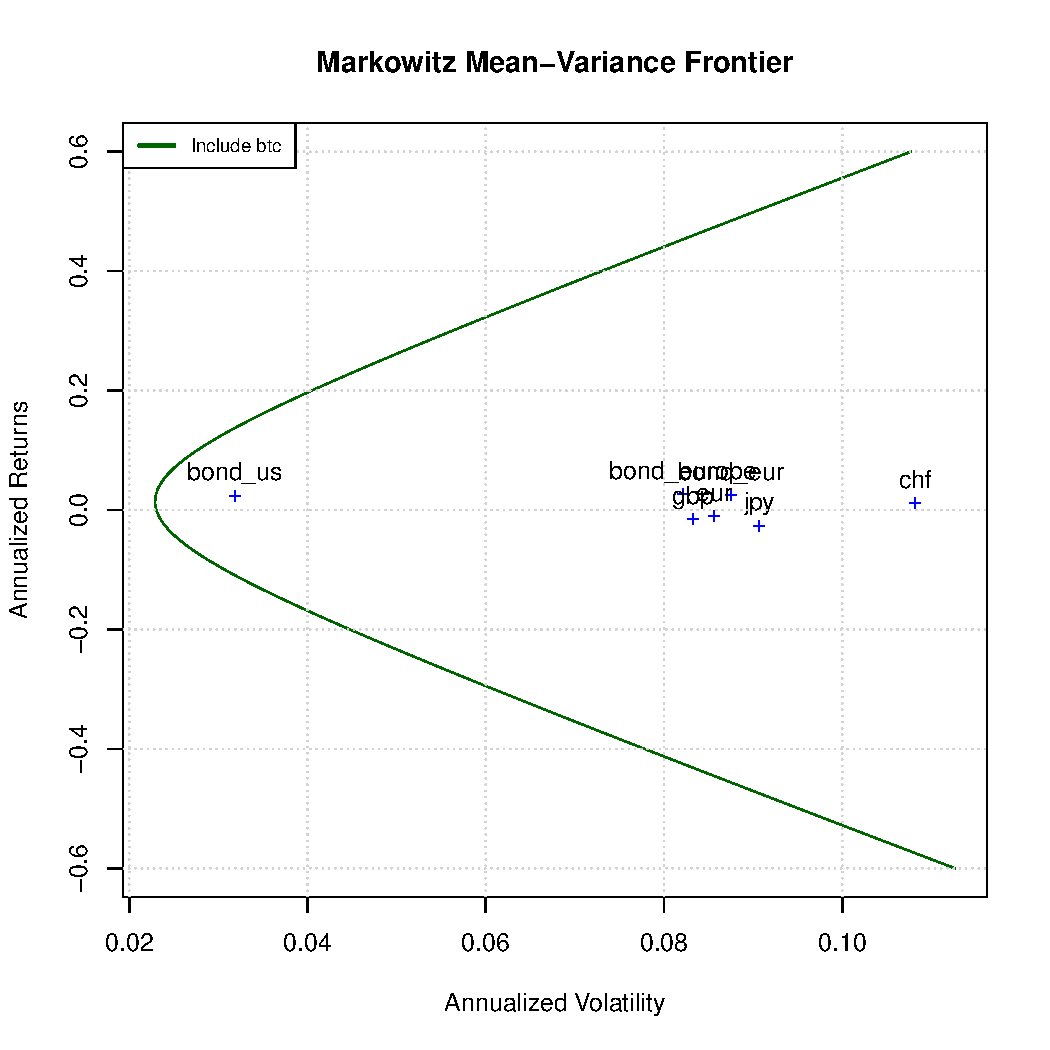
\includegraphics[width=0.6\textwidth]{Images/full_frontier.pdf}
	\caption{The Markowitz Mean-Variance frontier obtained from our portfolio of assets, that includes Bitcoin and allows short-selling.}
	\label{fig:full_frontier}
\end{figure}

In Figure \ref{fig:full_frontier} we can see what the portfolio frontier looks like for our portfolio of assets. 
It is interesting to notice how the curve divides the plane in two region: the area to the left of the line includes all those pairs $(\sigma, r)$ that are not attainable with our assets, since they have a volatility that is too low for that level of expected return. On the other hand, the region to the right of the portfolio frontier is made of all the pairs that are possible to obtain with a specific allocation $\mathbf{w}$ but that will never be chosen by an investor: moving to the left on the same level of return we eventually reach a point on the frontier. The portfolio represented by this point will dominate the one we started from in terms of risk, so it will always be a better choice.

We can proceed with the same argument arguing in terms of best return for a given level of risk: we can thus introduce the \textit{efficient} frontier. For every level of volatility that has two corresponding points on the portfolio frontier, only the one with the higher expected return will be chosen by an investor in our reference framework: hence only the top half of the curve (from the vertex and up) will form the \textit{efficient portfolio frontier}.

As a summary, let us keep in mind that any point in the volatility-expected return plane \textit{dominates} all the other portfolio allocations that are represented by points situated below and to the right of it. Conversely, that same point will be dominated by all other allocations above and to the left of it. 

Another mathematical perk of considering only the efficient top section is that it renders the frontier a \textit{bijective} function. Hence, for each (attainable) level of risk there is one and only one corresponding expected portfolio return, and vice-versa.


\subsection{Efficient Frontier with and without Bitcoin}

Let us now study how including Bitcoin in our portfolio of assets can help increase the diversification and obtain a higher (expected) return with a lower risk.

In Figure \ref{fig:efficient_frontier_comparison} we have plotted the efficient Markowitz frontier in all possible cases: including and excluding Bitcoin while allowing short-selling, and the same curves when short-selling is not allowed.

Comparing the two green lines, we can clearly see that the exclusion of short-selling does not penalize our efficient allocation by much. The same can be stated for the red and orange curves, which represent our portfolio when excluding the digital asset.
Thus, given our particular set of assets, allowing for short-selling does very little to improve the diversification of our portfolio.

Let us now take a look of what happens when we include Bitcoin in the reference portfolio: as we can see from Figure \ref{fig:efficient_frontier_comparison}, we get a significant improvement in the expected return when considering each level of risk . Equivalently, for the same level of return we have a noticeable decrease in the volatility of our portfolio.

%This is indeed one of the main result of this work

We can see some numerical proof of the diversification properties of adding Bitcoin to our portfolio in Table \ref{tab:markowitz_ret_on_vol} and Table	\ref{tab:markowitz_vol_on_ret}.

\begin{table}
\begin{tabular}{ccc}
\toprule
Volatility Level & Return without Bitcoin & Return including Bitcoin \\
\midrule
2,61\% & 3,00\% & 3,00\% \\
2,75\% & 3,89\% & 7,70\% \\
3,00\% & 4,59\% & 10,94\% \\
3,25\% & 5,05\% & 13,37\% \\
3,50\% & 5,43\% & 15,48\% \\
3,75\% & 5,76\% & 17,41\% \\
4,00\% & 6,06\% & 19,21\% \\
4,25\% & 6,34\% & 20,94\% \\
4,50\% & 6,61\% & 22,60\% \\
4,75\% & 6,87\% & 24,21\% \\
5,00\% & 7,12\% & 25,79\% \\
5,25\% & 7,37\% & 27,34\% \\
5,50\% & 7,61\% & 28,86\% \\
5,75\% & 7,85\% & 30,37\% \\
6,00\% & 8,08\% & 31,85\% \\
\bottomrule
\end{tabular}
\caption{Expected return for different levels of volatility, both including and excluding Bitcoin.}
\label{tab:markowitz_ret_on_vol}
\end{table}

\begin{table}
\begin{tabular}{lll}
	\toprule
	Return Level & Volatiliy without Bitcoin & Volatility including Bitcoin \\
	\midrule
	3,00\% & 2,61\% & 2,61\% \\
	3,50\% & 2,61\% & 2,67\% \\
	4,00\% & 2,61\% & 2,78\% \\
	4,50\% & 2,62\% & 2,96\% \\
	5,00\% & 2,63\% & 3,22\% \\
	5,50\% & 2,65\% & 3,55\% \\
	6,00\% & 2,67\% & 3,95\% \\
	6,50\% & 2,69\% & 4,40\% \\
	7,00\% & 2,71\% & 4,88\% \\
	7,50\% & 2,74\% & 5,39\% \\
	8,00\% & 2,77\% & 5,91\% \\
	8,50\% & 2,80\% & 6,45\% \\
	9,00\% & 2,84\% & 7,00\% \\
	9,50\% & 2,88\% & 7,56\% \\
	10,00\% & 2,92\% & 8,12\% \\
	10,50\% & 2,96\% & 8,69\% \\
	11,00\% & 3,01\% & 9,27\% \\
	11,50\% & 3,05\% & 9,85\% \\
	12,00\% & 3,10\% & 10,43\% \\
	12,50\% & 3,16\% & 11,01\% \\
	13,00\% & 3,21\% & 11,60\% \\
	13,50\% & 3,26\% & 12,19\% \\
	14,00\% & 3,32\% & 12,78\% \\
	14,50\% & 3,38\% & 13,37\% \\
	15,00\% & 3,44\% & 13,96\% \\
	\bottomrule
\end{tabular}
\caption{Volatility for different level of expected portfolio return, both including and excluding Bitcoin.}
\label{tab:markowitz_vol_on_ret}
\end{table}


\begin{figure}
	\centering
	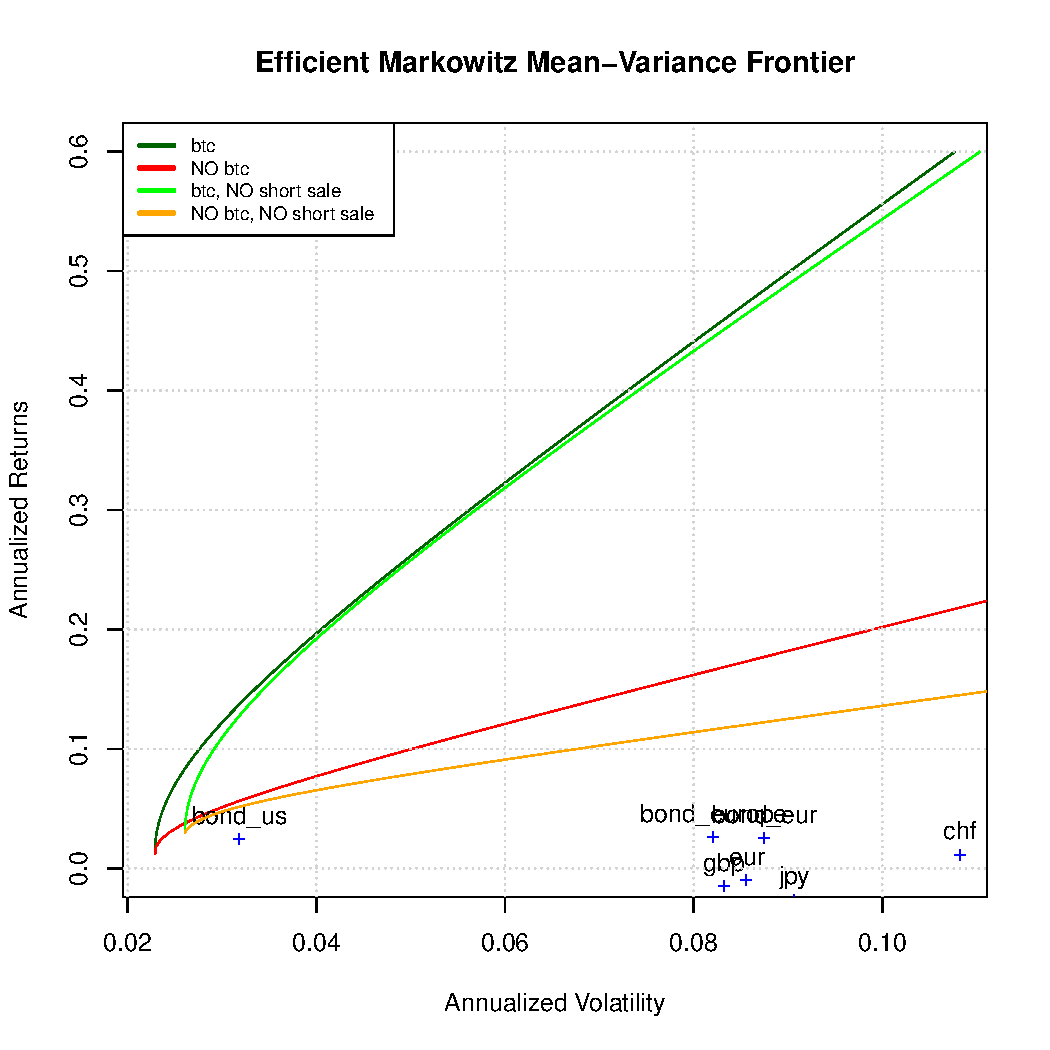
\includegraphics[width=0.6\textwidth]{Images/efficient_frontier.pdf}
	\caption{The \textit{Efficient} Markowitz Mean-Variance frontier obtained from our portfolio of assets, both including and excluding Bitcoin and with short-selling or not.}
	\label{fig:efficient_frontier_comparison}
\end{figure}


\subsection{Portfolio Allocation}
We have so far seen the implications of introducing the digital asset in our portfolio in terms of improvement in the expected return and of lowering the overall portfolio risk.
Let us now take a look at how Markowitz MPT allocates the money in the different assets.

To do so, we can plot the values of $\mathbf{w}$ as resulting from \eqref{eq:markowitz_opt} for different levels of volatilities ( and hence returns).



\section{Portfolio Optimization with CVaR as a Risk Measure}
We have so far studied the problem of optimal portfolio allocation through Markowitz MPT, considering the portfolio volatility as a proxy for its risk.
This is only one of the possible choices in a more general framework in which the optimization problem to be solved maintains the same constraints but has a  different objective function. We can reformulate \eqref{eq:markowitz_opt} as follows:

\begin{subequations}
	\label{eq:general_opt}
	\begin{align}
	%	\label{eq:mark_min}
	&\!\min_{\mathbf{w}\in \mathbb{R}^{N}}     &    & PtfRisk(\mathbf{w}) \\
	%	\label{eq:mark_weights}
	& \text{subject to}   &   & \mathbf{e}^T\mathbf{w} = 1 ,\\
	%	\label{eq:mark_return}
	&                 &       & \mathbf{r}^T\mathbf{w} = r_{target},\label{eq:constraint2} \\
	%	\label{eq:mark_noshort}
	&		   &      & w_{i} \geq 0, \text{for} \: i = 1\dots N. 
	\end{align}
\end{subequations}

where we have substituted the portfolio volatility with a general measure of the portfolio risk as a function of the weights $\mathbf{w}$.

Using the portfolio volatility as risk measure has its perks and downsides: it is an intuitive and simple way to evaluate how the possible returns vary from the expected value but it takes into account both the positive and the negative deviation from the mean. Thus, a high volatility may be caused by a few extremely high returns that are anything but something to avoid and penalize.
For this reason, the notion of \textit{semi-volatility} was introduced to only consider variations towards lower returns than the one expected. This solution however is not very popular.

A more common approach is to measure risk based on the quantile of the loss distribution \footnote{Depending on how the returns are expressed, we have different ways to compute the loss. In particular, considering the time interval $[0, T]$, for log-returns $r_{log}=log(S_T/S_0)$ the loss is simply the opposite $Loss_{log} = - r_{log}$ while for $r_\% = S_T/S_0$  the loss is $Loss_\% = 1 - r_\%$. As usual we indicate by $S_t$ the price  of the asset or the value of the portfolio at time $t$.}. The \textit{Value-at-Risk} of level $\alpha$ for a loss distribution is precisely defined as the quantile of order $\alpha$.  
VaR is a vastly popular and common way to measure the so called ``tail-risk'': the intrinsic risk contained in loss events that happen very rarely. 
Its advantage is that it considers only the downside of the expected return as opposed to what the volatility does.

However, VaR has drawbacks as its mathematical definition does not make it a \textit{coherent measure of risk}. Specifically, it lacks the property of sub-additivity: the VaR of two different portfolios  considered as one may be greater than the sum of the two single VaRs. This is in direct contradiction with the principle of diversification.

\textbf{aggiungere appendice dove si definisce una misura coerente di rischio con le 3/4 proprietà}

\chapter{Conclusions}
\label{chpr:conclusion}


The aim of this work was to study the properties of Bitcoin as a digital asset.

In Chapter \ref{chpr:corr_analysis} we studied the empirical correlation between the returns of Bitcoin and of 16 other assets, grouped in 4 different classes (stock indexes, bonds indexes, currencies and commodities). We found out that the correlation not only is low, but it also is not significantly different from zero, from a statistical point of view. The same holds for the rolling correlation computed in the time span of our data (mid July 2010 to early November 2018).

Then, in Chapter \ref{chpr:calibration} we obtained the same correlation matrix through the calibration of three continuous asset price models: Merton's jump diffusion, Heston's stochastic volatility and Bates's stochastic volatility with jumps in the price process.
For all three, the resulting correlation structure closely resembles the one computed in Chapter \ref{chpr:corr_analysis}: this indicates that there is no real need for a sophisticated model to obtain a feel for what the level of the correlation of Bitcoin with other assets is.

The fact that returns of Bitcoin are not correlated with those of more standard assets lead us to consider the possibility of including the digital asset in an investment portfolio.
In Chapter \ref{chpr:markowitz} we compare the performances of two portfolios, in a Markowitz framework: the first only includes the standard assets while the second also contains Bitcoin. The difference in terms of increased returns or lowered risk is dramatic. We can see this both by looking at the graph of the efficient frontiers and at the numerical results.
We performed the same analysis implementing the daily CVaR at 95\% as the portfolio risk measure to specifically account for the tails of the historical distribution, obtaining very similar results to the previous case.
In general, investing 3\% to 5\% of our wealth in Bitcoin proved to be extremely beneficial.

\bigskip

A possible further study can be to analyse the correlation between the most relevant crypto-currencies in the same way that we did here with standard assets. We expect to find that the correlation levels are pretty high and thus it would not prove to be beneficial to include more than one in an investment portfolio. 

Another interesting subject of study for a deeper investigation of the asset allocation problem would be to implement a Black and Litterman approach, which allows to also take into account the investor's assumptions on the market returns of the assets.


\bigskip
Even more than the  results of the whole numerical analysis that we performed in this work, we believe that the properties, the  infrastructure and the community behind Bitcoin make it a cut above other crypto-currencies and stand tall against scepticism and misunderstandings, rendering it the only resilient and durable crypto-investment.
 
\bigskip



%
%The aim of this thesis is to give an introduction to the Schnorr signature algorithm, starting from the mathematics and the cryptography behind the scheme, and present some of its amazing applications to Bitcoin, detailing the benefits and the improvements that would arise from its deployment. We started with a brief but thorough description of the mathematical structures (Chapter \ref{chpr:math}) and cryptographic primitives (Chapter \ref{chpr:ecc}) that underpin digital signature schemes based on elliptic curve cryptography. In Chapter \ref{chpr:dss} we presented both ECDSA and Schnorr algorithm, respectively the one actually implemented in Bitcoin and the one that is under development. We compared the two schemes, investigating ECDSA lacks and Schnorr benefits, that ranged from security to efficiency. In particular we focused on the linearity property, that turned out to be the key for the higher level construction presented in Chapter \ref{chpr:application}.
%\\
%We have seen how to traduce utilities already implemented in Bitcoin in terms of Schnorr signatures: multi-signature schemes are implemented through MuSig (Section \ref{musig}), whose main advantage is to recover key aggregation; threshold signatures can be deployed through the protocols presented in Section \ref{threshold}, that makes them indistinguishable from a single signature; the last application we studied has been adaptor signature and its benefits to cross-chain atomic swaps and to the Lightning Network.
%
%\bigskip
%\noindent
%The immediate benefits that Schnorr would bring to Bitcoin are improved efficiency (smaller signatures, batch validation, cross-input aggregation) and privacy (multi-signatures and threshold signatures would be indistinguishable from a single signature), leading also to an enhancement in fungibility. All this applications would be possible in a straightforward way after the introduction of Schnorr, that could be brought to Bitcoin through a soft-fork\footnote{Improvements in the protocol have to be made without consensus split.}: the fact that Schnorr is superior to ECDSA in every aspect hopefully will ease the process.
%
%\bigskip
%\noindent
%The last thing we would like to point out is that, by no means, the applications presented in the present work are the unique benefits that Schnorr could bring to Bitcoin. More complex ideas take the names of Taproot \cite{Taproot} and Graftroot \cite{Graftroot}, and are built on top of the concepts of MAST and Pay-to-Contract: through these constructions it would be possible, in the cooperative case, to hide completely the redeem script, presenting a single signature (no matter how complex the script is). For how soft forks need to be implemented after SegWit (i.e. with an upgrade of the version number), there is incentive to develop as many innovations as possible altogether (the presence of too many version numbers with little differences would constitute a lack of privacy): for this reason, it is probable that Schnorr will come to life accompanied by Taproot. 
%\\
%Hopefully, we have convinced the reader that Schnorr (and Bitcoin!) is worth being studied, providing also the tools to properly understand further features and innovations other than the ones presented. Moreover, we hope that you are now motivated not only to delve deeper in the technical side of Bitcoin, but also to approach it from other sides, to fully appreciate its disruptiveness and make yourself an idea of what Bitcoin is and which possibilities it hides.



%----------------------------------------------------------------------------------------
%	THESIS CONTENT - APPENDICES
%----------------------------------------------------------------------------------------
\bibliographystyle{apalike}
\bibliography{Bibliography/my_bibliography}

\appendix
\chapter{Characteristic Function of a Compound Poisson Process }
\label{app:A}


By definition, the characteristic function of a random variable $X$ is given by:
\begin{equation}
\label{eq:chf_def}
	\phi_{X}(u) = \mathbb{E}[e^{iuX}].
\end{equation}

Let us first consider a simple Poisson process $N_t$ of parameter $\lambda$. At each time $t >0$, $N_t$ has a discrete distribution that follows:
\begin{equation}
\mathbb{P}( N_t = n) = e^{-\lambda t}\frac{(\lambda t)^n}{n!} ,\: n = 0,1,2,...
\end{equation}

Since $N_t$ is a \textit{discrete} random variable, the expectation in \eqref{eq:chf_def} amounts to a sum over all the possible values of $N_t$:

\begin{equation*} 
	\begin{split}
	\phi_{N_t}(u) & = \mathbb{E}[e^{iu N_t}] = \sum_{n=0}^{\infty} e^{iun} \mathbb{P}( N_t = n)\\
	&= \sum_{n=0}^{\infty}e^{iun}e^{-\lambda t}\frac{(\lambda t)^n}{n!}\\
	&= e^{-\lambda t} \sum_{n=0}^{\infty}\frac{(\lambda t e^{iu})^n}{n!}.\\
	\end{split}
\end{equation*}

Using the definition of exponential $e^x  = \sum_{n=0}^{\infty} \frac{x^n}{n!}$ we then get the final result:
\begin{equation*} 
	\begin{split}
	\phi_{N_t}(u) & = e^{-\lambda t} e^{\lambda t e^{iu})}\\
	& = e^{\lambda t (e^{iu}-1)}.
	\end{split}
\end{equation*}

Let us consider now a compound Poisson process defined by 
\begin{equation}
	X_t = \sum_{i=1}^{N_t} Y_i
\end{equation}
where $Y_i$ are i.i.d. and have density expressed by the function $f_Y(y)$.

\bigskip
To compute the characteristic function of $X_t$ we can follow the same steps as in the simple Poisson case, but in addition we use the Theorem of Total Expectation to first simplify the expression and then proceed exploiting the i.i.d property:
\begin{equation*} 
	\begin{split}
	\phi_{X_t}(u) & = \mathbb{E}[e^{iu X_t}]\\
	&= \sum_{n=0}^{\infty} \mathbb{E}[e^{iu X_t}| N_t = n] \mathbb{P}( N_t = n)\\
	&= \sum_{n=0}^{\infty} \mathbb{E}[\prod_{i=1}^{N_t}e^{iu Y_i}| N_t = n] \mathbb{P}( N_t = n)\\
	& = \sum_{n=0}^{\infty} \prod_{i=1}^{n}\mathbb{E}[e^{iu Y_i}| N_t = n] \mathbb{P}( N_t = n)\\
	&= \sum_{n=0}^{\infty} (\mathbb{E}[e^{iu Y}])^n \mathbb{P}( N_t = n)\\
	&= \sum_{n=0}^{\infty}(\phi_Y(u))^n e^{-\lambda t}\frac{(\lambda t)^n}{n!}\\
	&= e^{-\lambda t}\sum_{n=0}^{\infty}\frac{(\lambda t \, \phi_Y(u))^n}{n!}\\
	&=e^{\lambda t (\phi_Y(u)-1)}.
	\end{split}
\end{equation*}

\chapter{Histograms}
\label{app:hist}

In the following pages we include the histograms of the distributions of the log-returns for each of the assets in our dataset. We superimpose to the histograms the graphs of the density functions obtained using the three models of Merton, Heston and Bates with the calibrated parameters shown in Tables \ref{tab:merton_params}, \ref{tab:heston_params} and \ref{tab:bates_params}.

We can see that given our results from the calibration, Heston and Bates better approximate the empirical distribution of the returns in all cases.

\begin{figure}
	\small
	\centering
	\begin{subfigure}{0.44\textwidth}
		\centering
		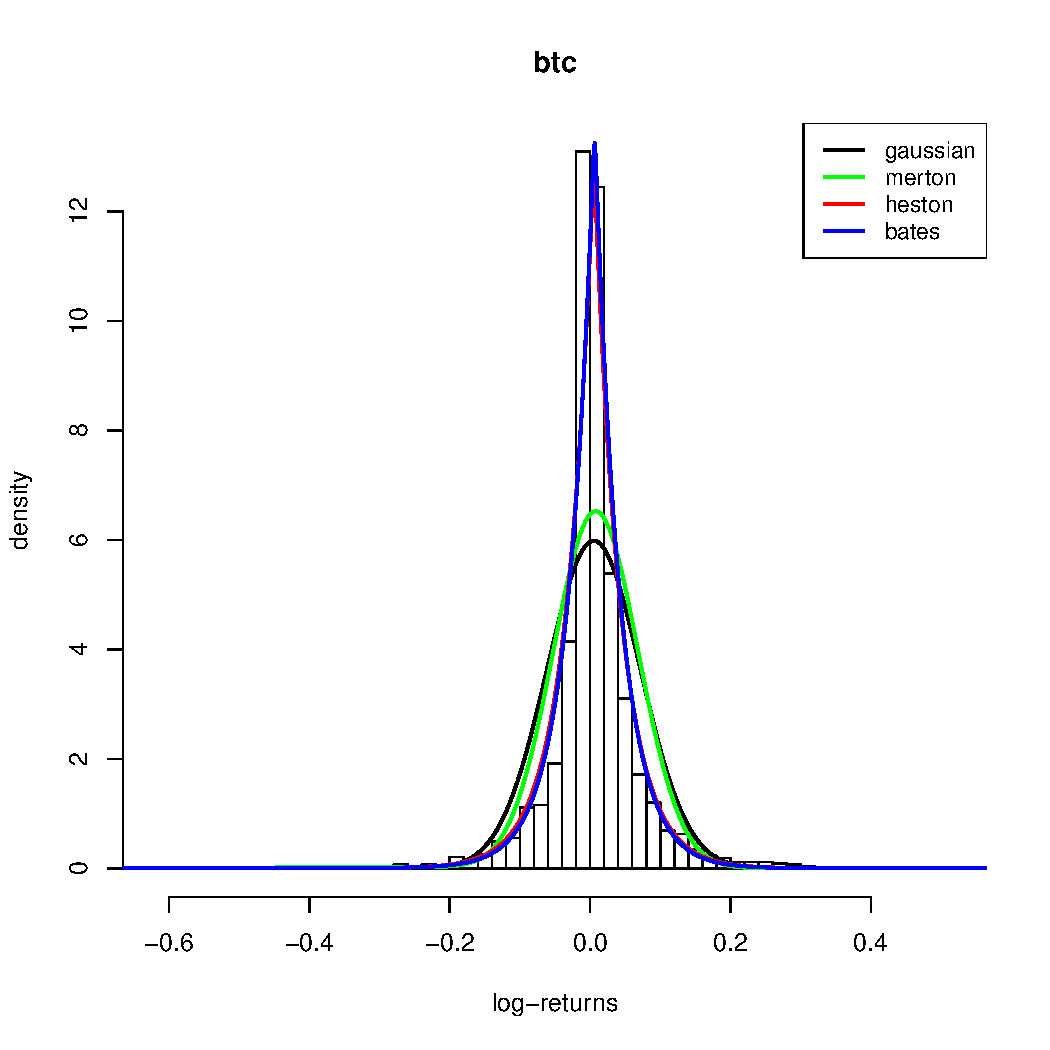
\includegraphics[width=\linewidth]{Images/hist_btc.pdf}
		\caption{Bitcoin}
	\end{subfigure}
	\begin{subfigure}{0.44\textwidth}
		\centering
		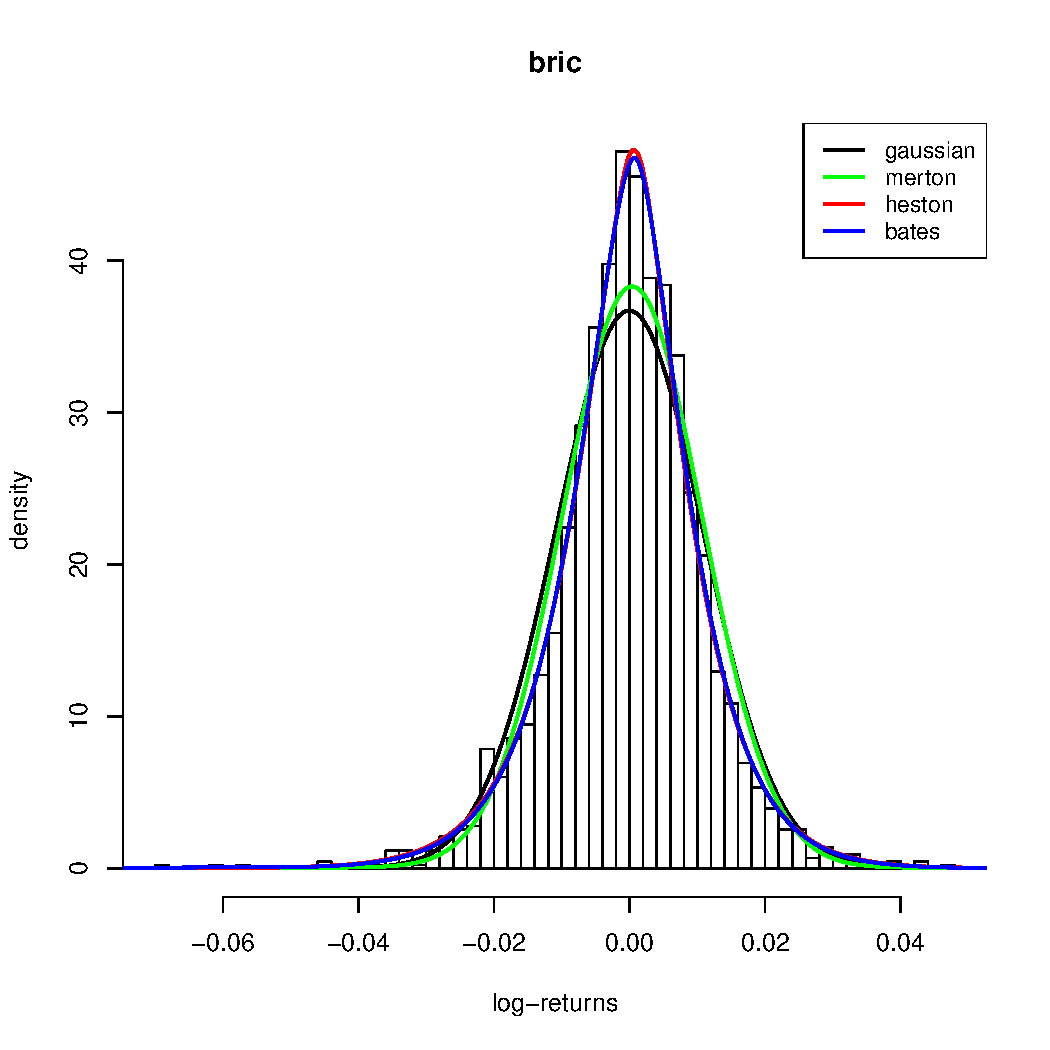
\includegraphics[width=\linewidth]{Images/hist_bric.pdf}
		\caption{Bric index}
	\end{subfigure}
	\\
	\begin{subfigure}{0.44\textwidth}
		\centering
		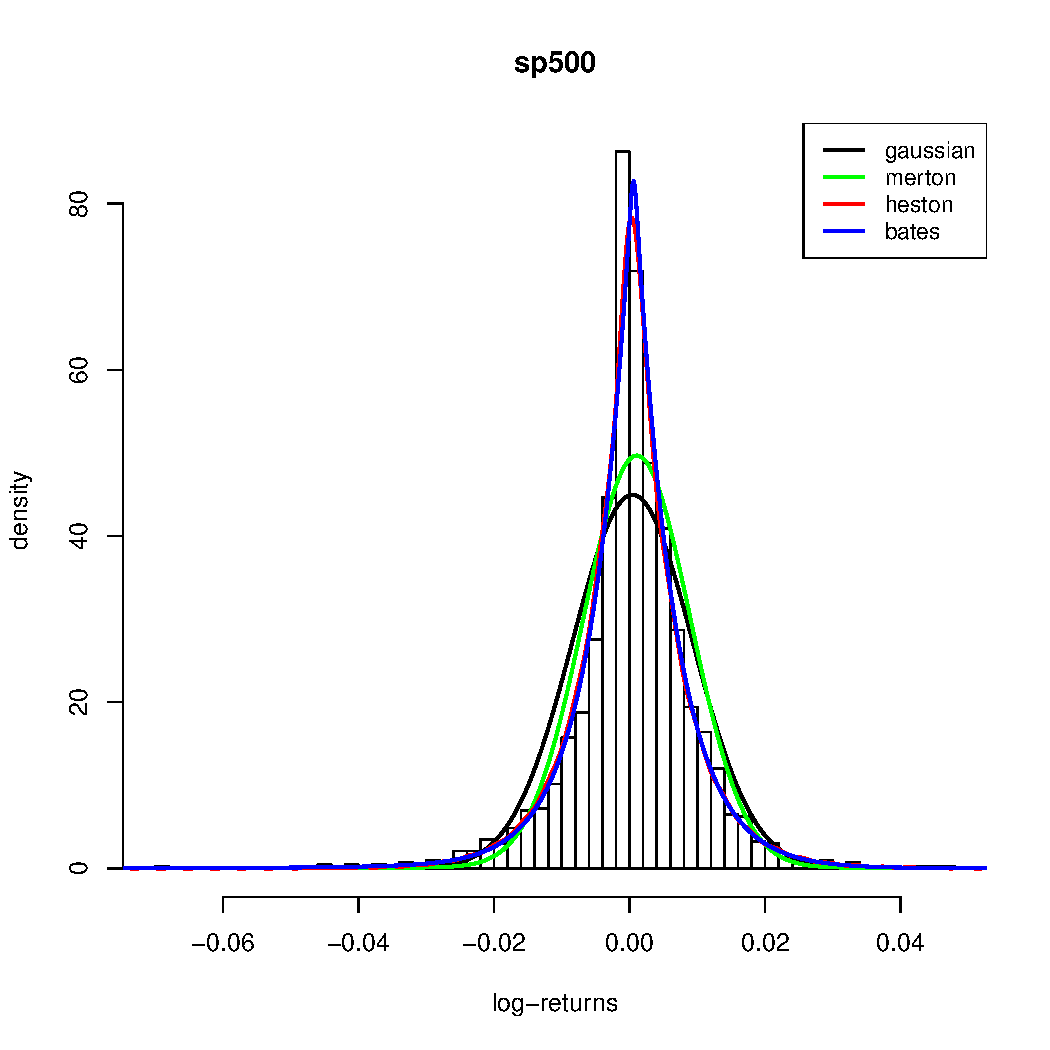
\includegraphics[width=\linewidth]{Images/hist_sp500.pdf}
		\caption{S\&P500}
	\end{subfigure}
	\begin{subfigure}{0.44\textwidth}
		\centering
		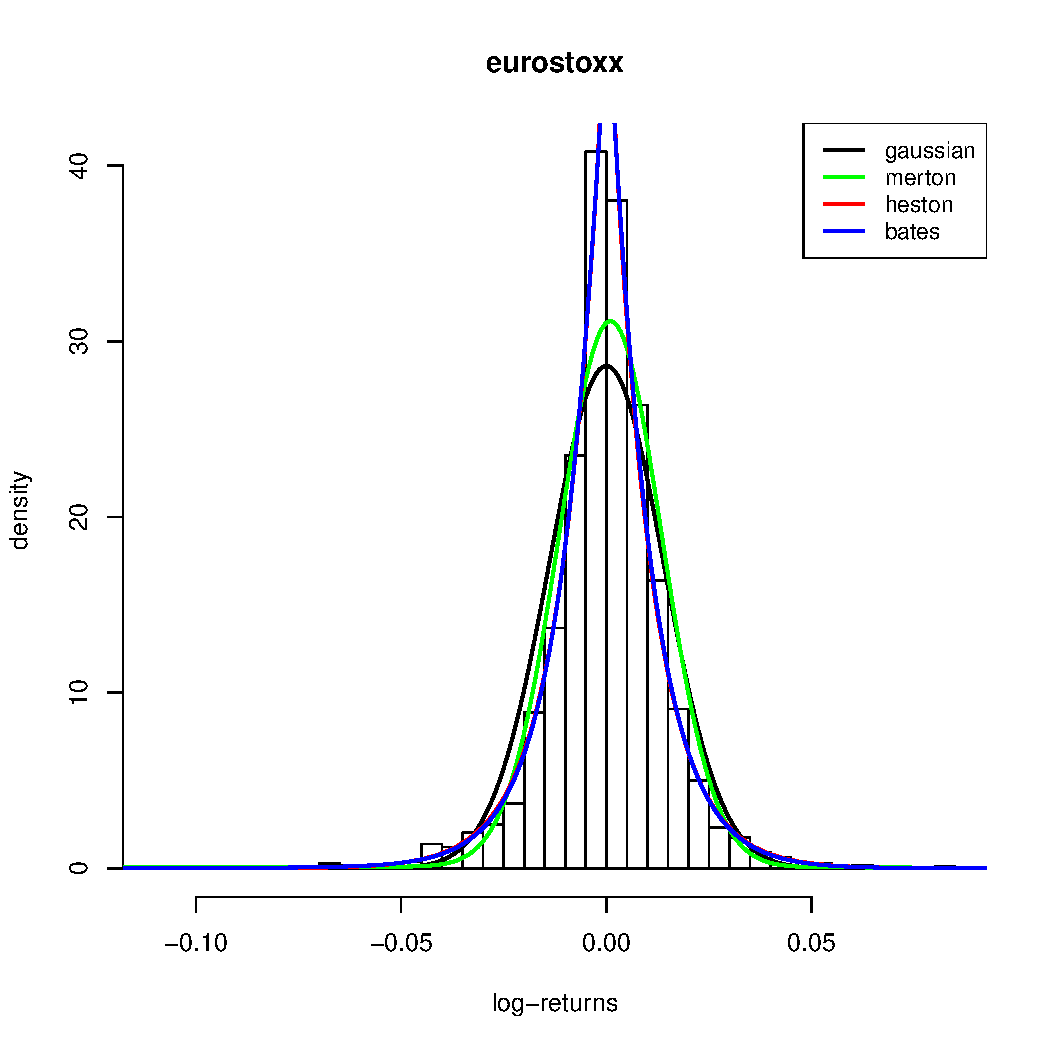
\includegraphics[width=\linewidth]{Images/hist_eurostoxx.pdf}
		\caption{Eurostoxx50}
	\end{subfigure}
	\caption[Histrogram and densities of the results (1/3)]{Histogram of the log-returns and pdf for the three models we calibrated and the Gaussian line as reference.[1/3]}
	\label{fig:hist_1}
	
\end{figure}





\begin{figure}
	\small
	\centering
	\begin{subfigure}{0.44\textwidth}
		\centering
		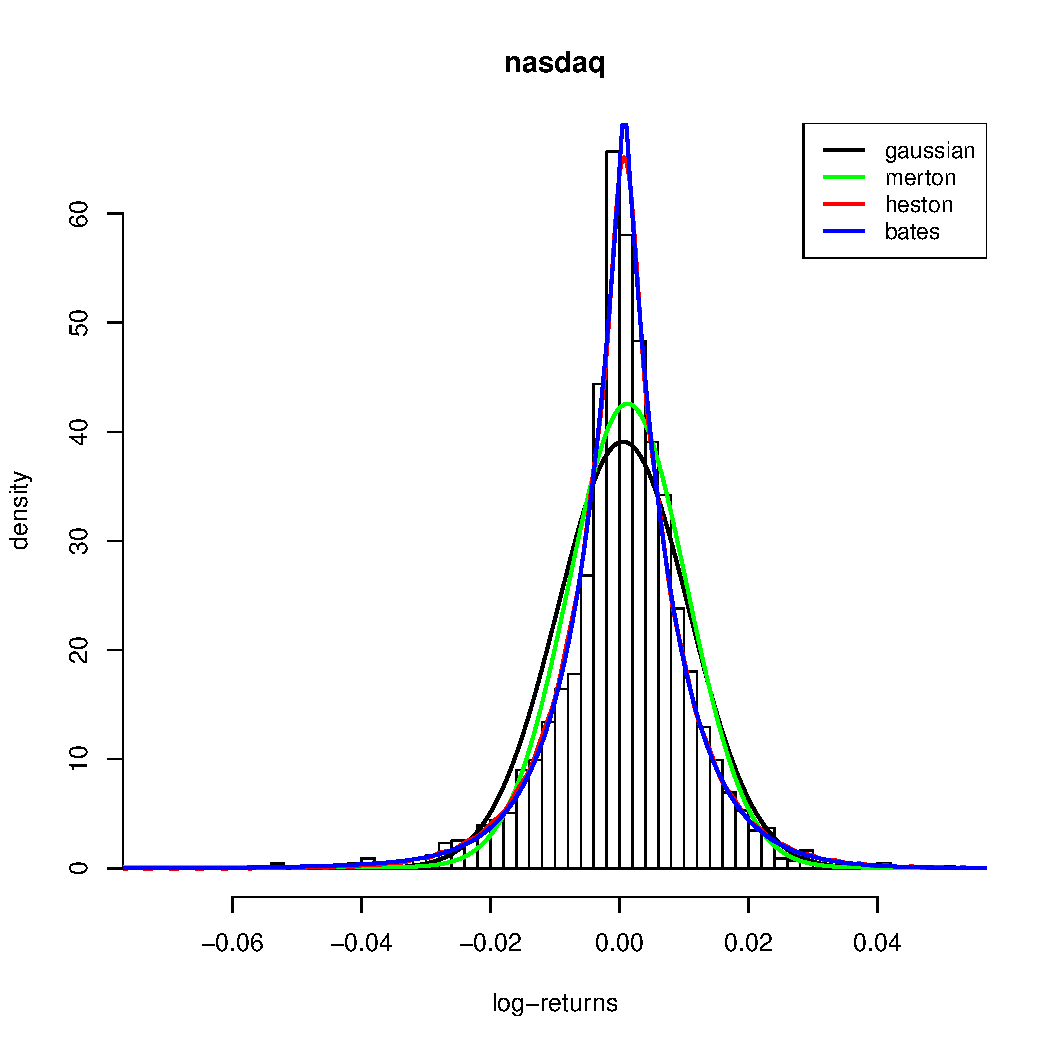
\includegraphics[width=\linewidth]{Images/hist_nasdaq.pdf}
		\caption{Nasdaq}
	\end{subfigure}
	\begin{subfigure}{0.44\textwidth}
		\centering
		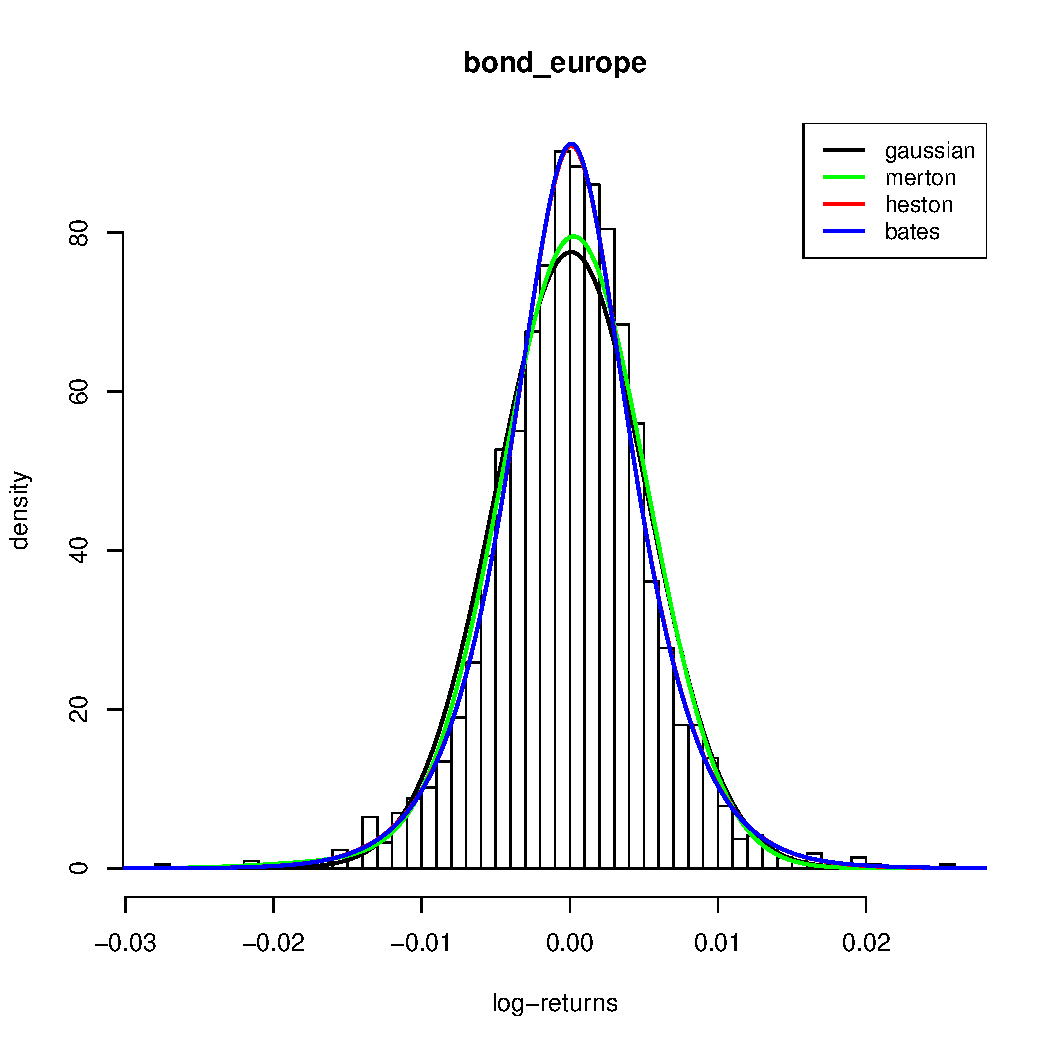
\includegraphics[width=\linewidth]{Images/hist_bond_europe.pdf}
		\caption{Bond Europe}
	\end{subfigure}

\begin{subfigure}{0.44\textwidth}
	\centering
	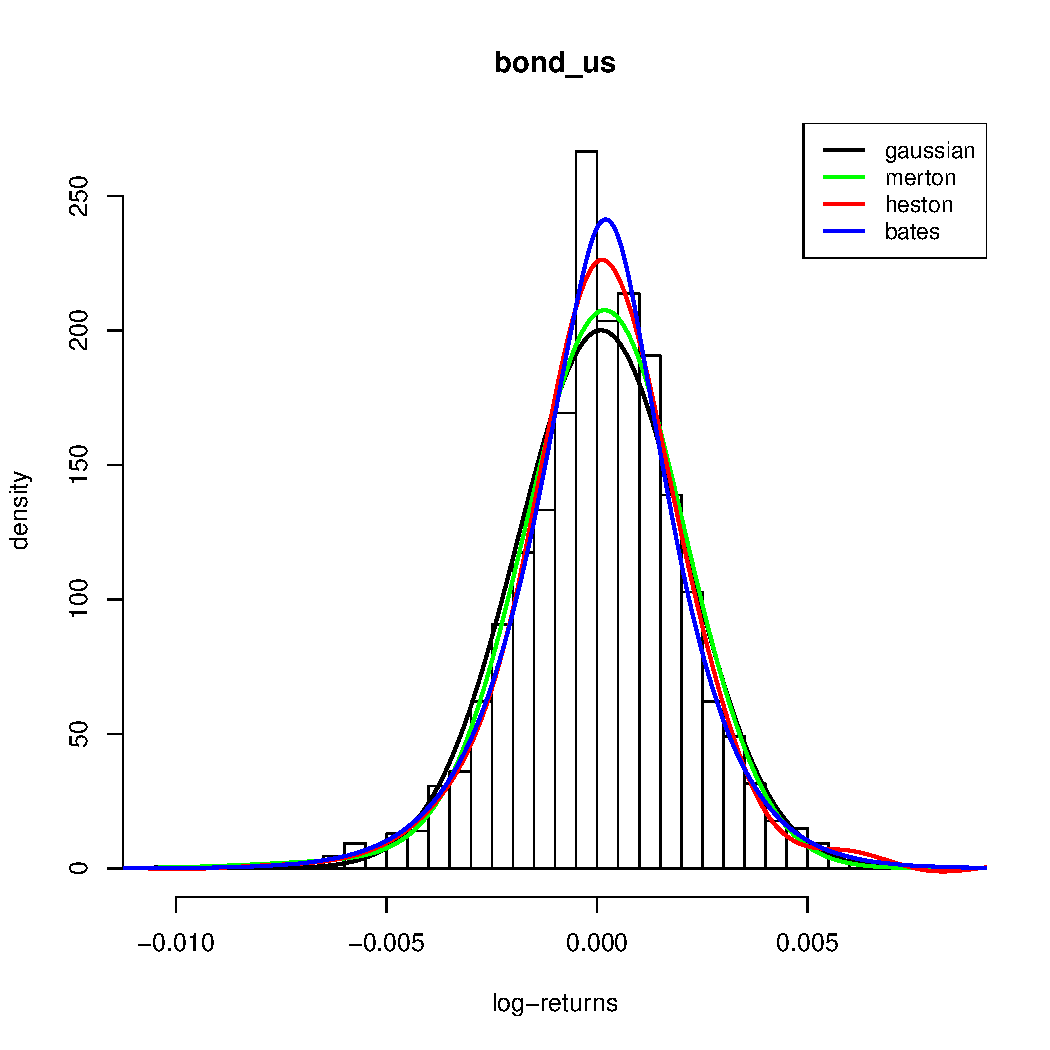
\includegraphics[width=\linewidth]{Images/hist_bond_us.pdf}
	\caption{Bond US}
\end{subfigure}
\begin{subfigure}{0.44\textwidth}
	\centering
	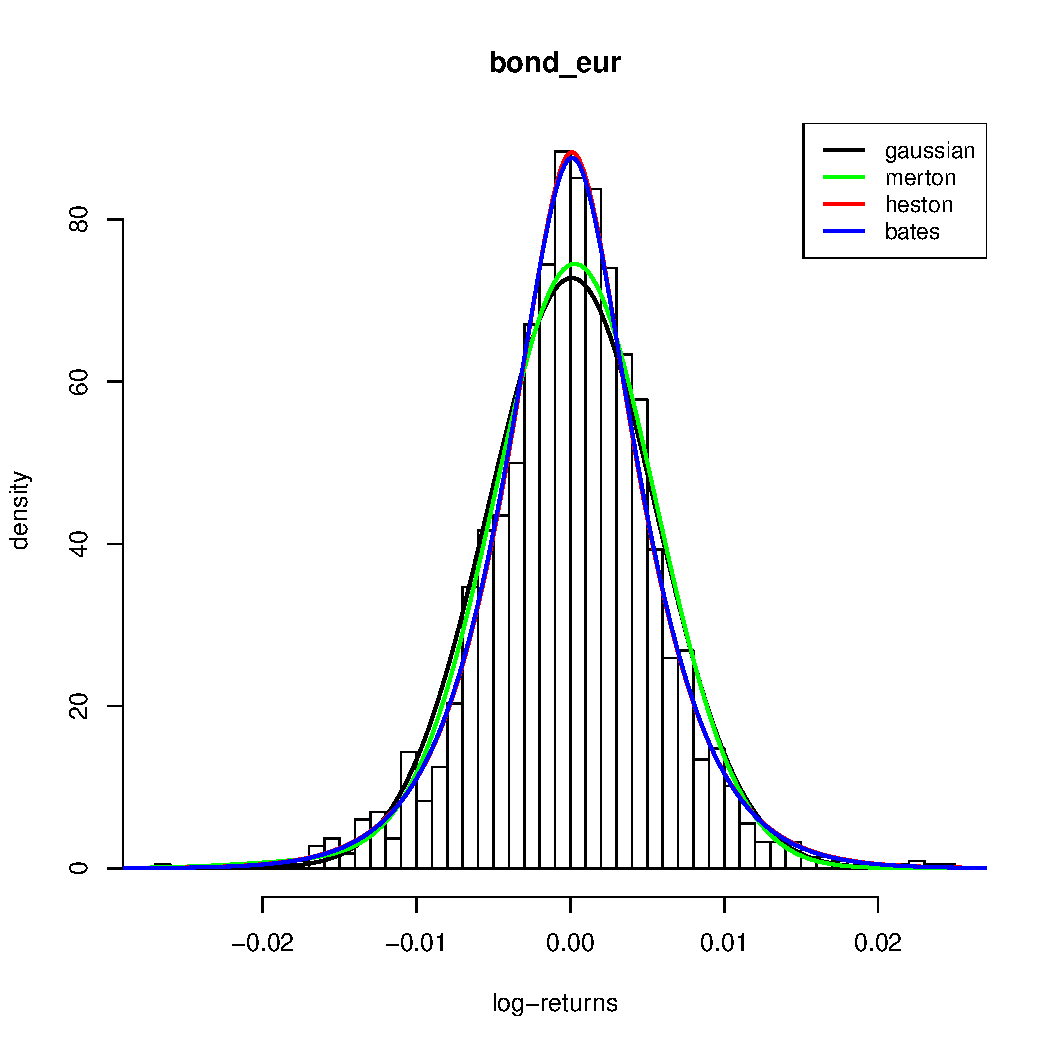
\includegraphics[width=\linewidth]{Images/hist_bond_eur.pdf}
	\caption{Bond EUR}
\end{subfigure}

\begin{subfigure}{0.44\textwidth}
	\centering
	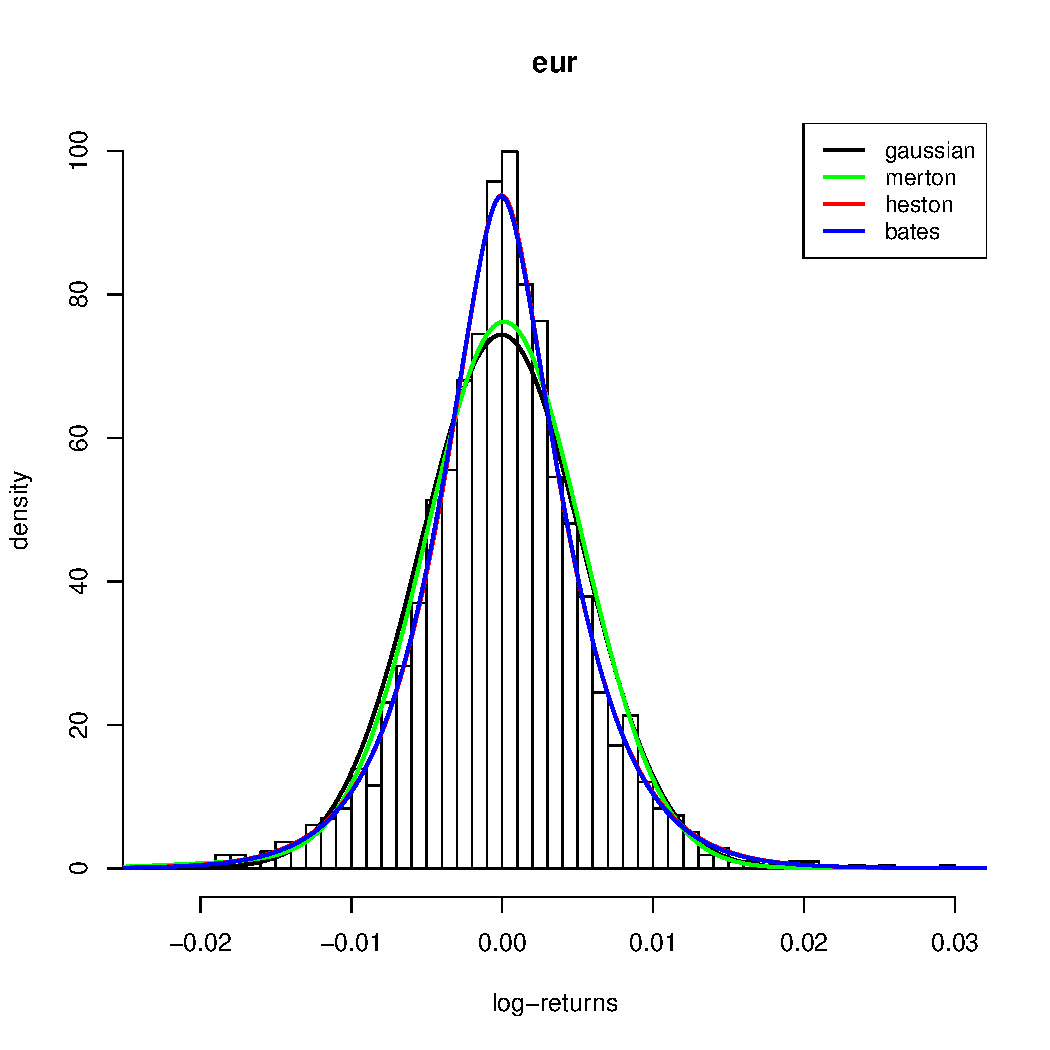
\includegraphics[width=\linewidth]{Images/hist_eur.pdf}
	\caption{EUR/USD}
\end{subfigure}
\begin{subfigure}{0.44\textwidth}
	\centering
	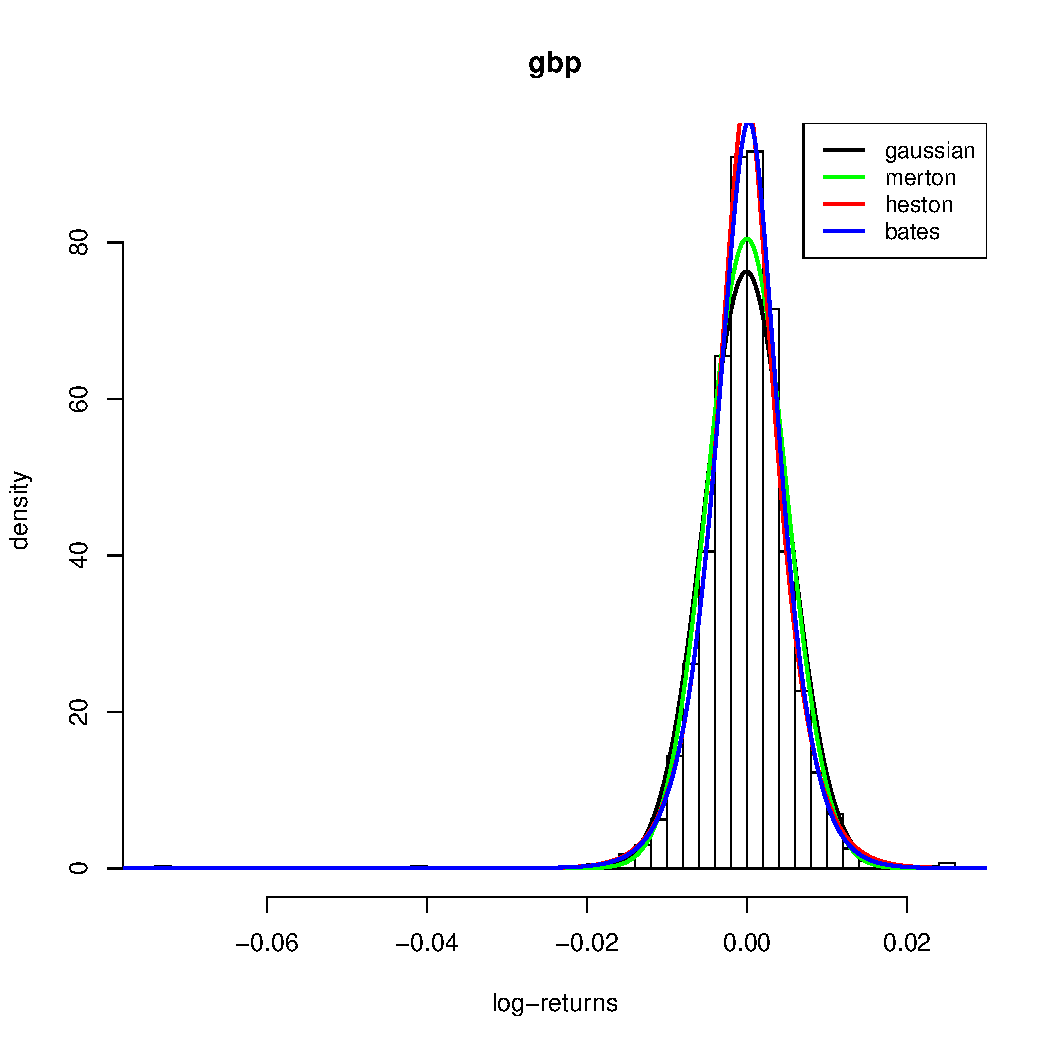
\includegraphics[width=\linewidth]{Images/hist_gbp.pdf}
	\caption{GBP/USD}
\end{subfigure}

\caption[Histrogram and densities of the results (2/3)]{Histogram of the log-returns and pdf for the three models we calibrated and the Gaussian line as reference.[2/3]}
\label{fig:hist_2}
\end{figure}


\begin{figure}
	\small
	\centering
	\begin{subfigure}{0.44\textwidth}
		\centering
		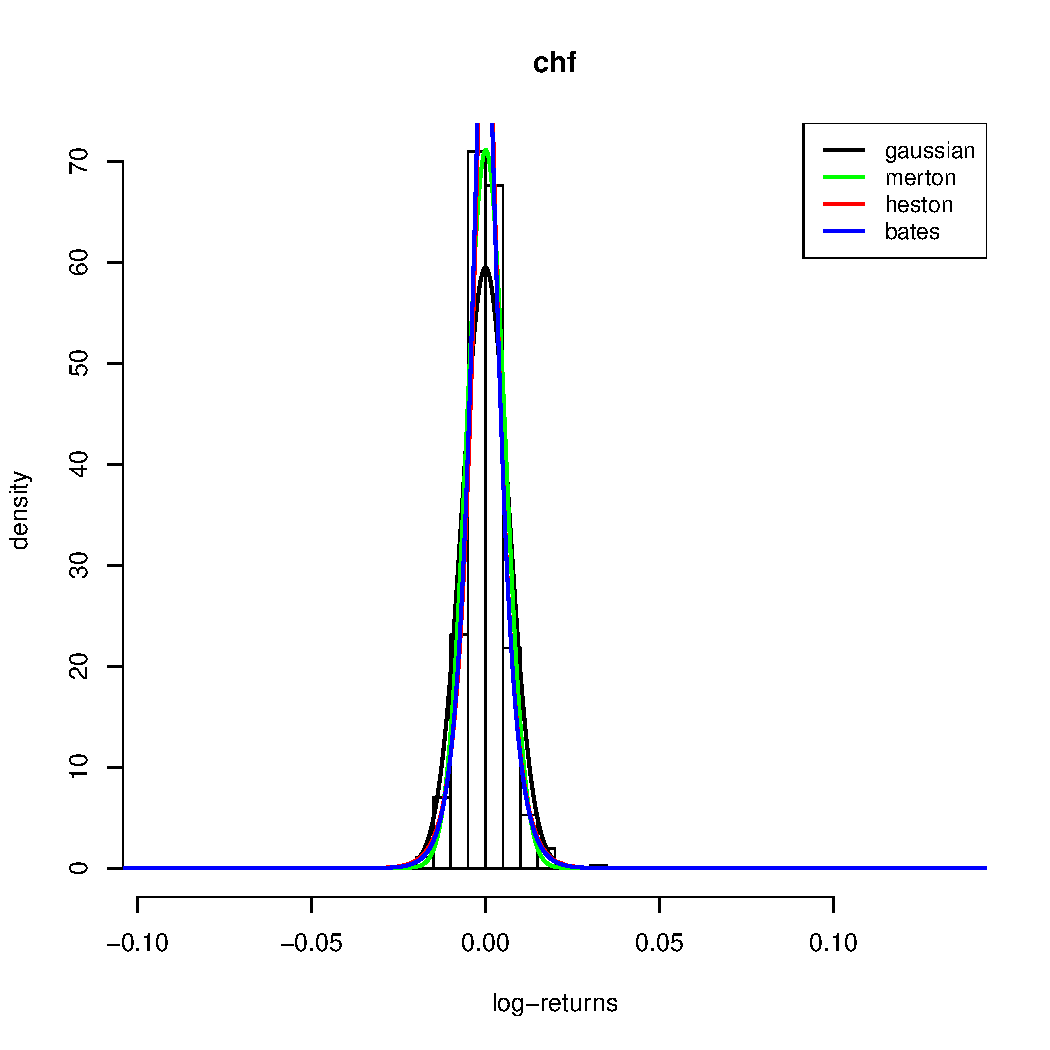
\includegraphics[width=\linewidth]{Images/hist_chf.pdf}
		\caption{CHF/USD}
	\end{subfigure}
	\begin{subfigure}{0.44\textwidth}
		\centering
		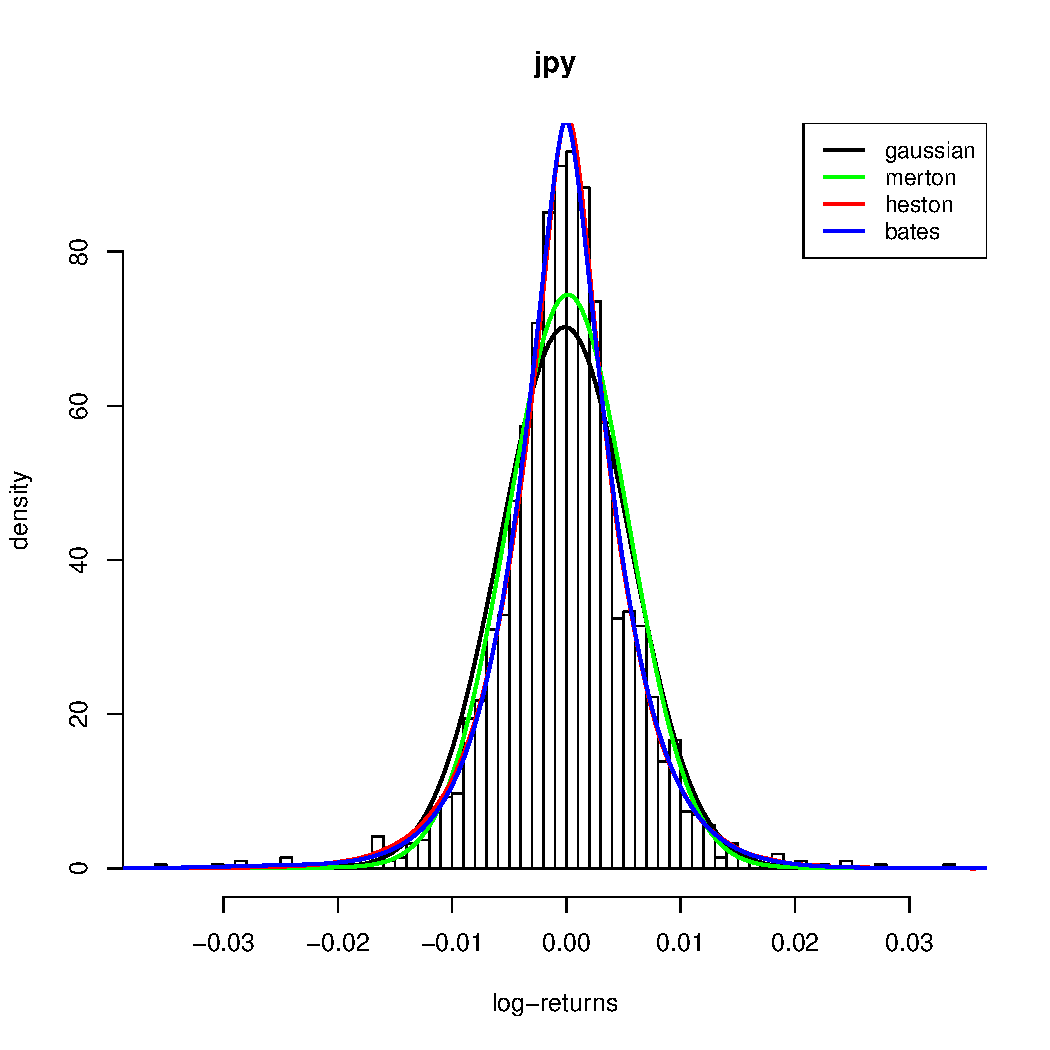
\includegraphics[width=\linewidth]{Images/hist_jpy.pdf}
		\caption{JPY/USD}
	\end{subfigure}
	
	\begin{subfigure}{0.44\textwidth}
		\centering
		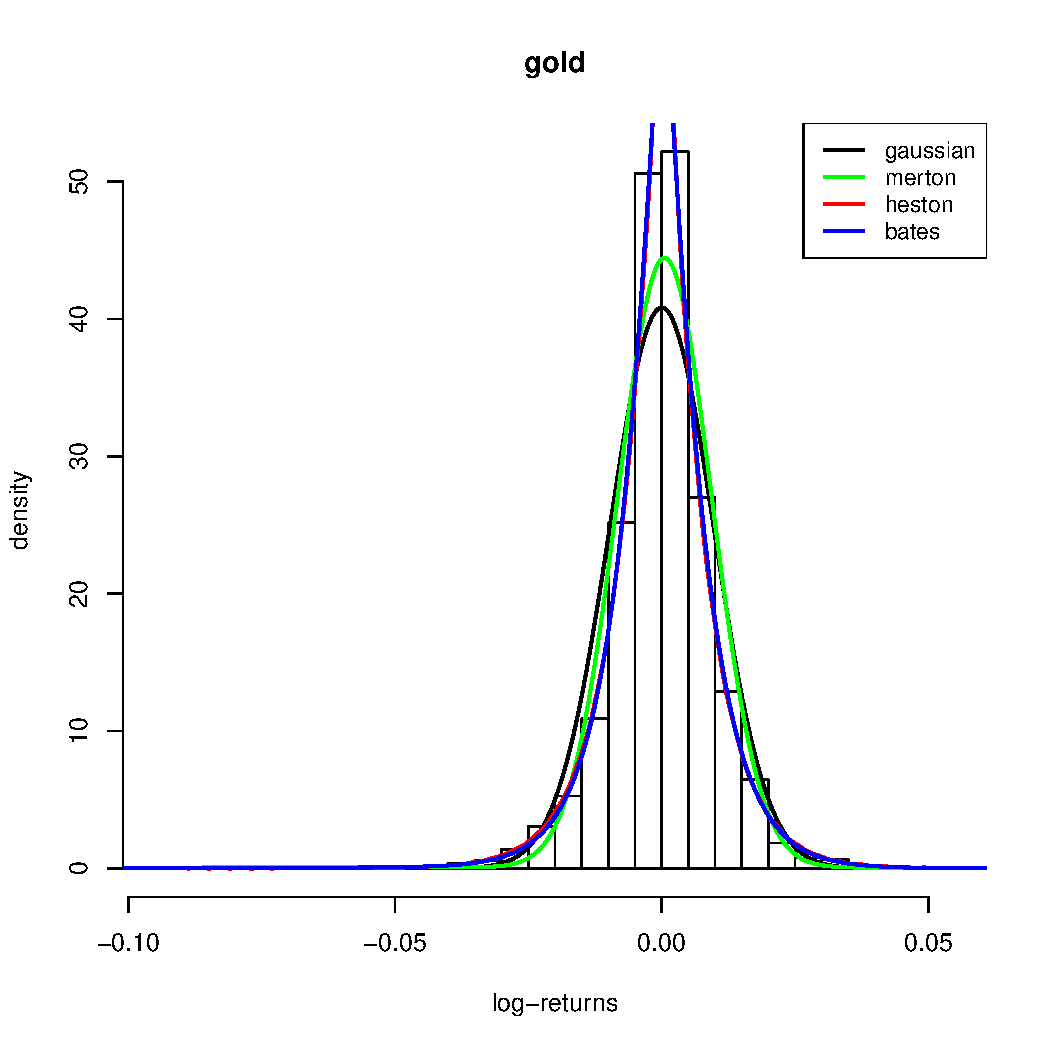
\includegraphics[width=\linewidth]{Images/hist_gold.pdf}
		\caption{Gold}
	\end{subfigure}
	\begin{subfigure}{0.44\textwidth}
		\centering
		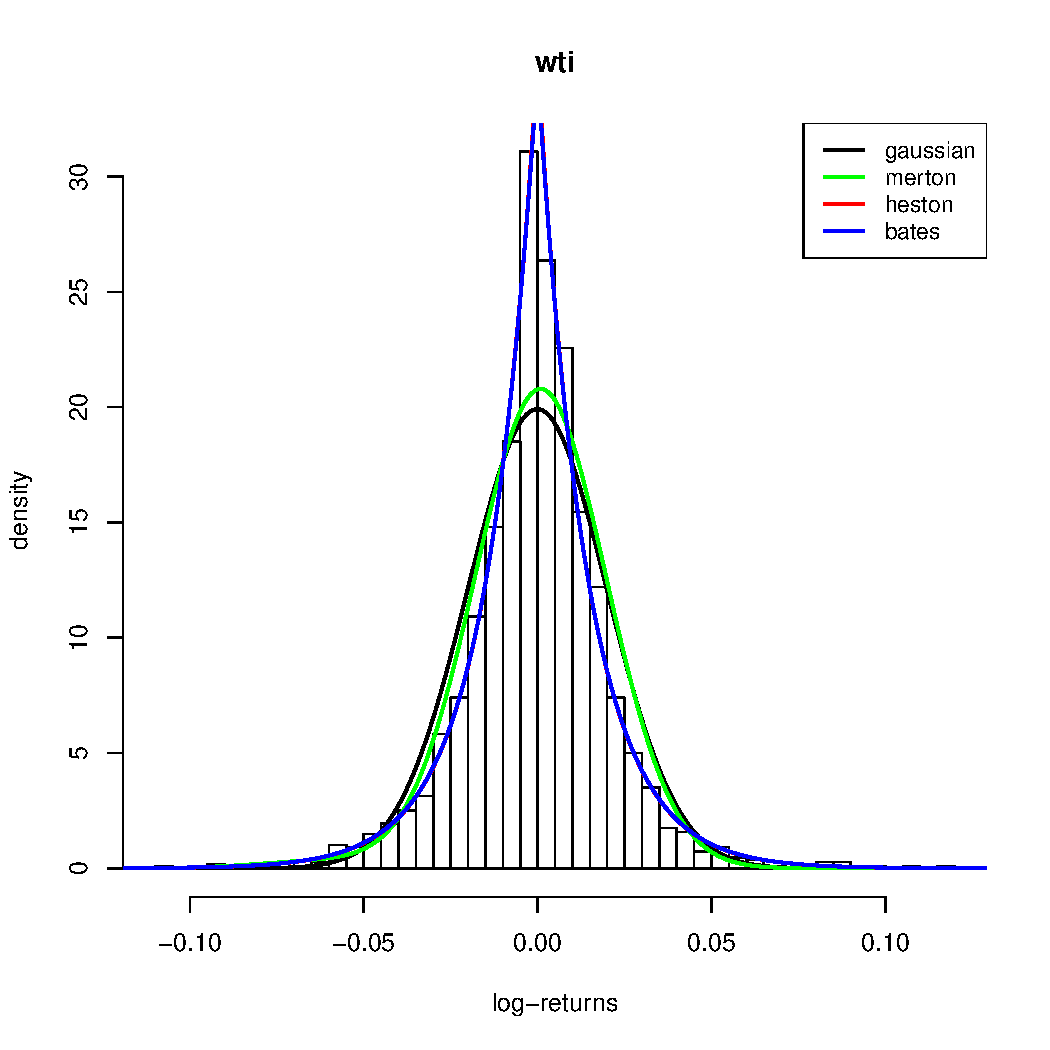
\includegraphics[width=\linewidth]{Images/hist_wti.pdf}
		\caption{Wti oil}
	\end{subfigure}
	
	\begin{subfigure}{0.44\textwidth}
		\centering
		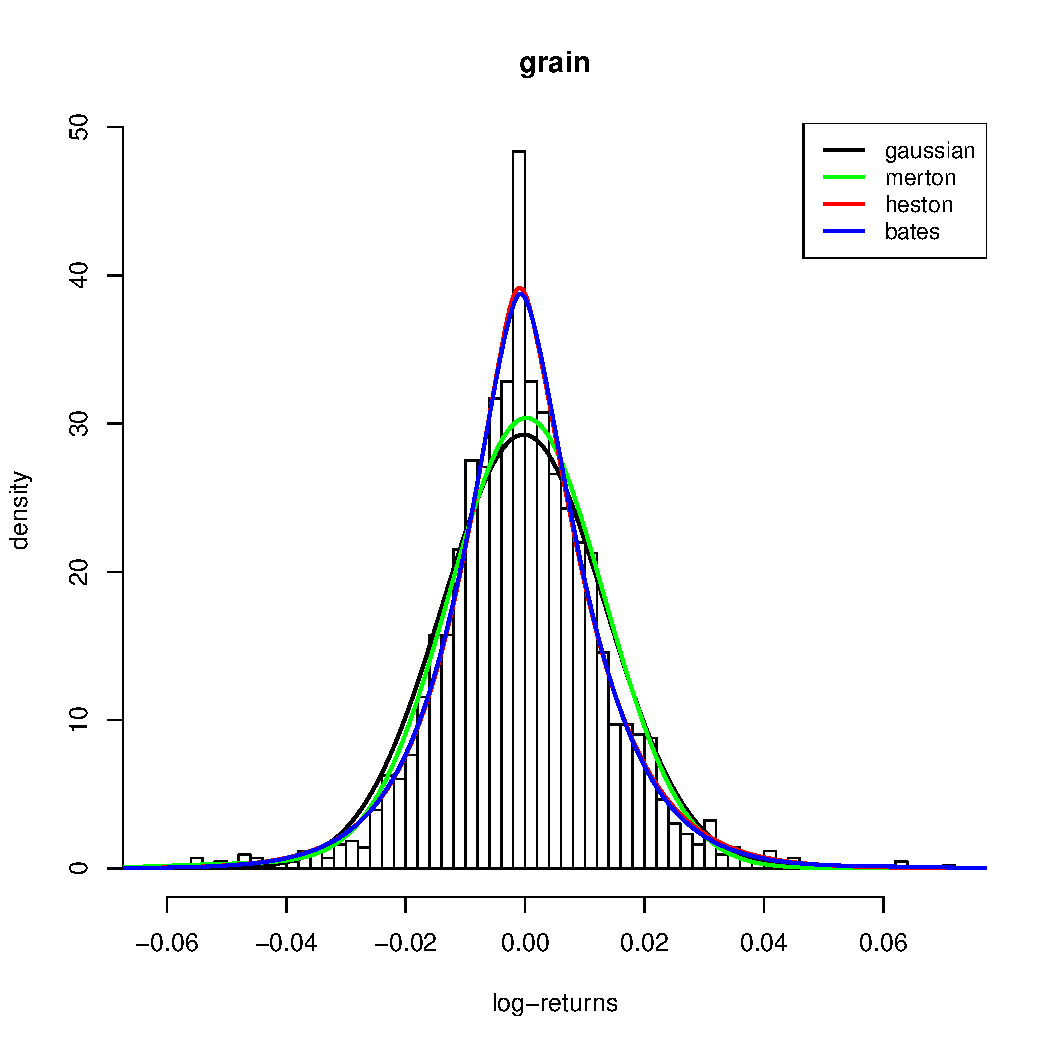
\includegraphics[width=\linewidth]{Images/hist_grain.pdf}
		\caption{Grain}
	\end{subfigure}
	\begin{subfigure}{0.44\textwidth}
		\centering
		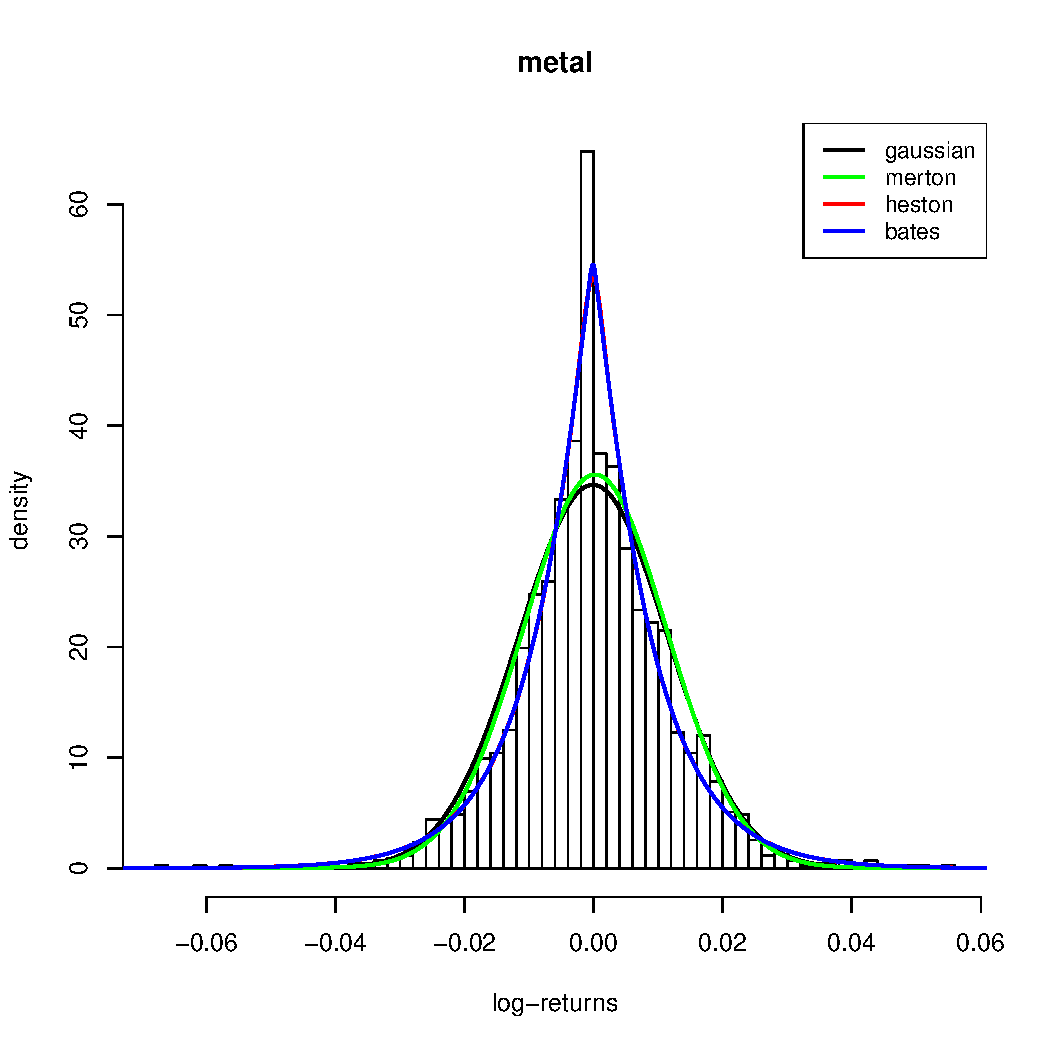
\includegraphics[width=\linewidth]{Images/hist_metal.pdf}
		\caption{Metals}
	\end{subfigure}
	
	\caption[Histrogram and densities of the results (3/3)]{Histogram of the log-returns and pdf for the three models we calibrated and the Gaussian line as reference. [3/3]}
	\label{fig:hist_3}
\end{figure}

%\\
%\begin{subfigure}{0.44\textwidth}
%	\centering
%	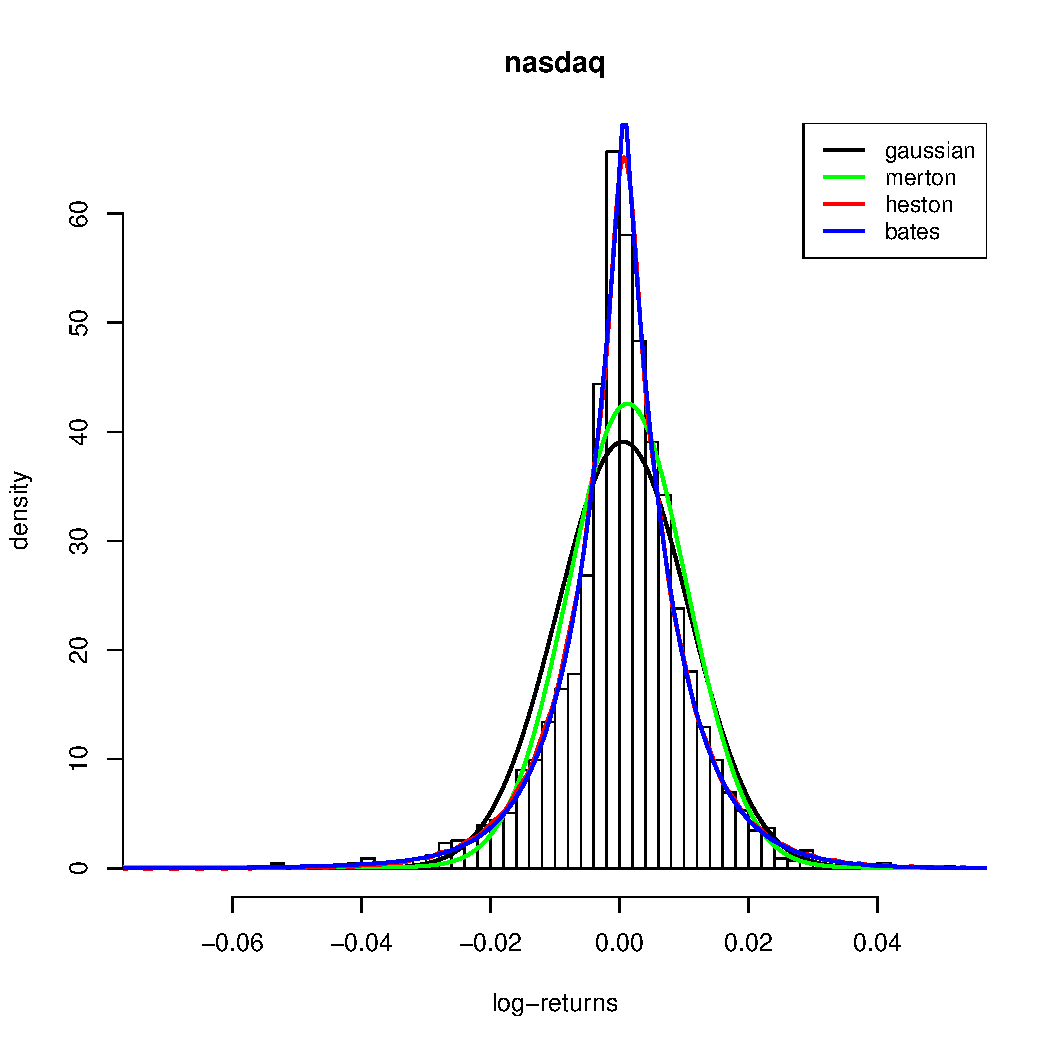
\includegraphics[width=\linewidth]{Images/hist_nasdaq.pdf}
%	\caption{text}
%\end{subfigure}
%\begin{subfigure}{0.44\textwidth}
%	\centering
%	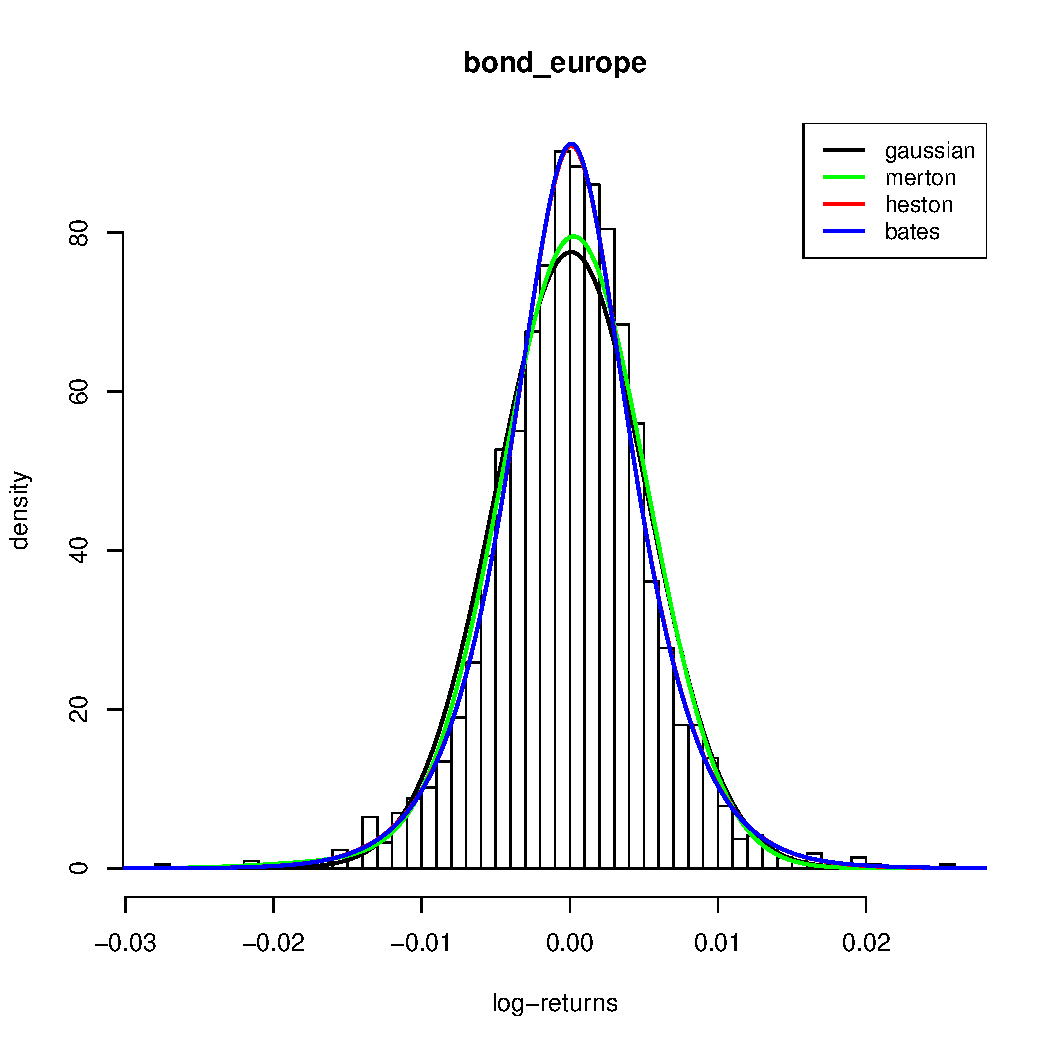
\includegraphics[width=\linewidth]{Images/hist_bond_europe.pdf}
%	\caption{text}
%\end{subfigure}

%	\hspace{0mm}
%\subfloat[Nasdaq]{   
%	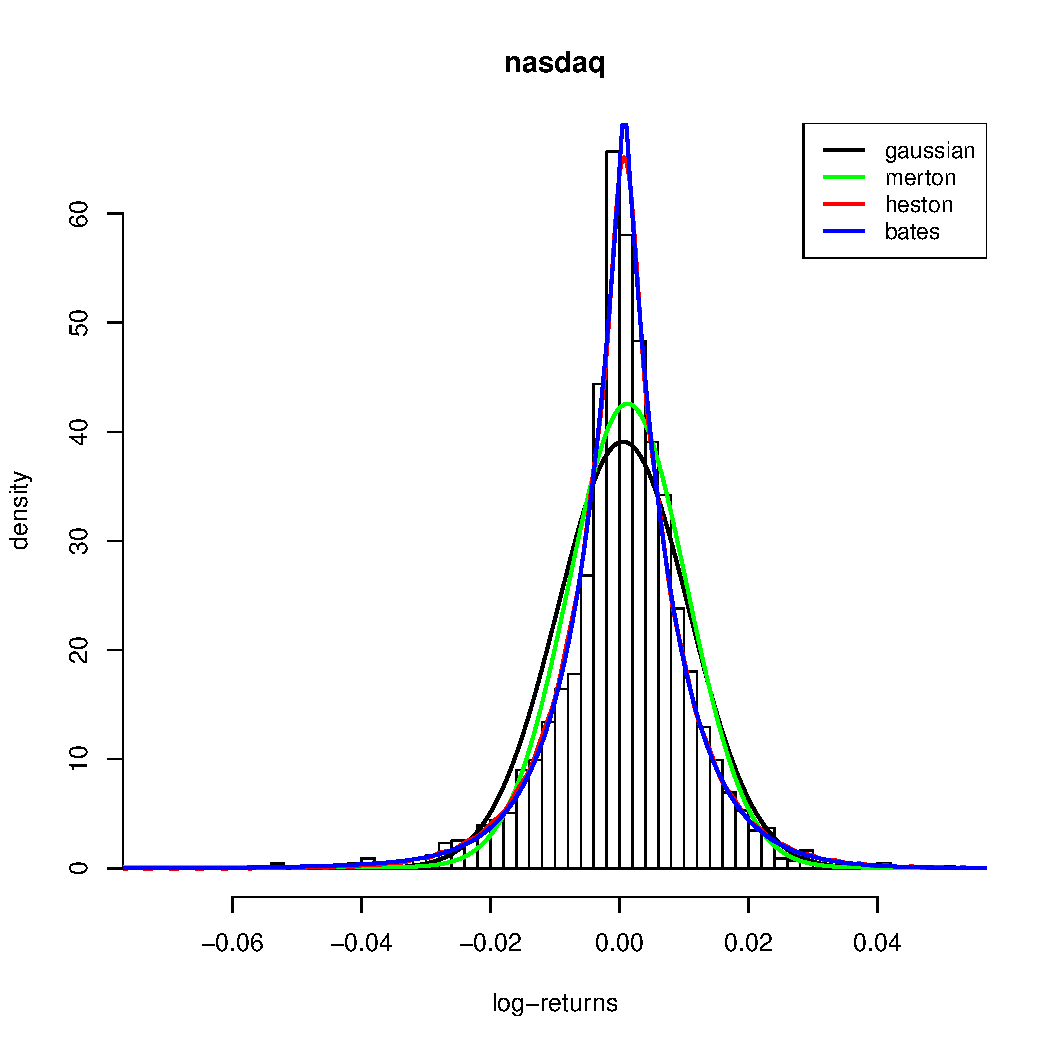
\includegraphics[height=0.3\textheight]{Images/hist_nasdaq.pdf}
%}
%\subfloat[Bond Europe]{
%	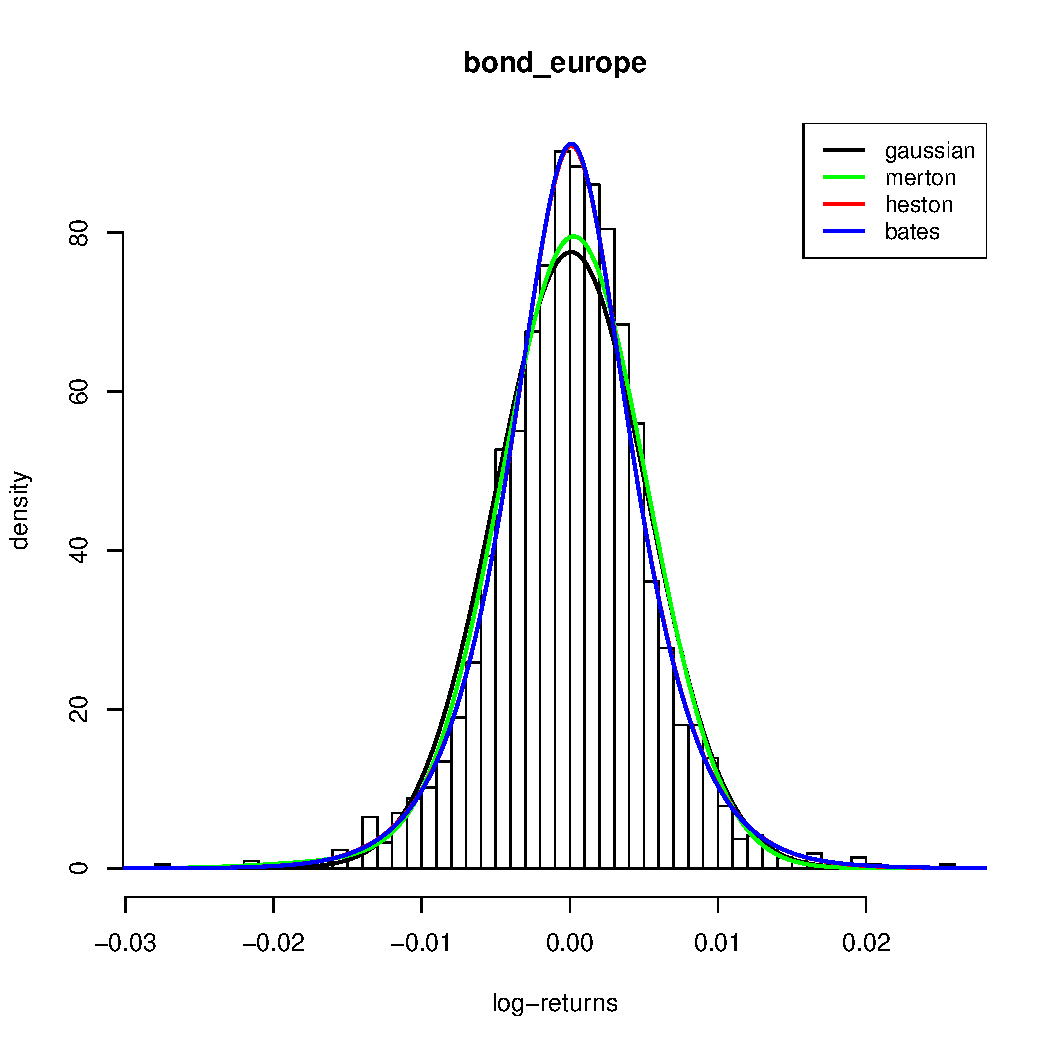
\includegraphics[height=0.3\textheight]{Images/hist_bond_europe.pdf}
%}

%	\hspace{0mm}
%\subfloat[Bond US]{   
%	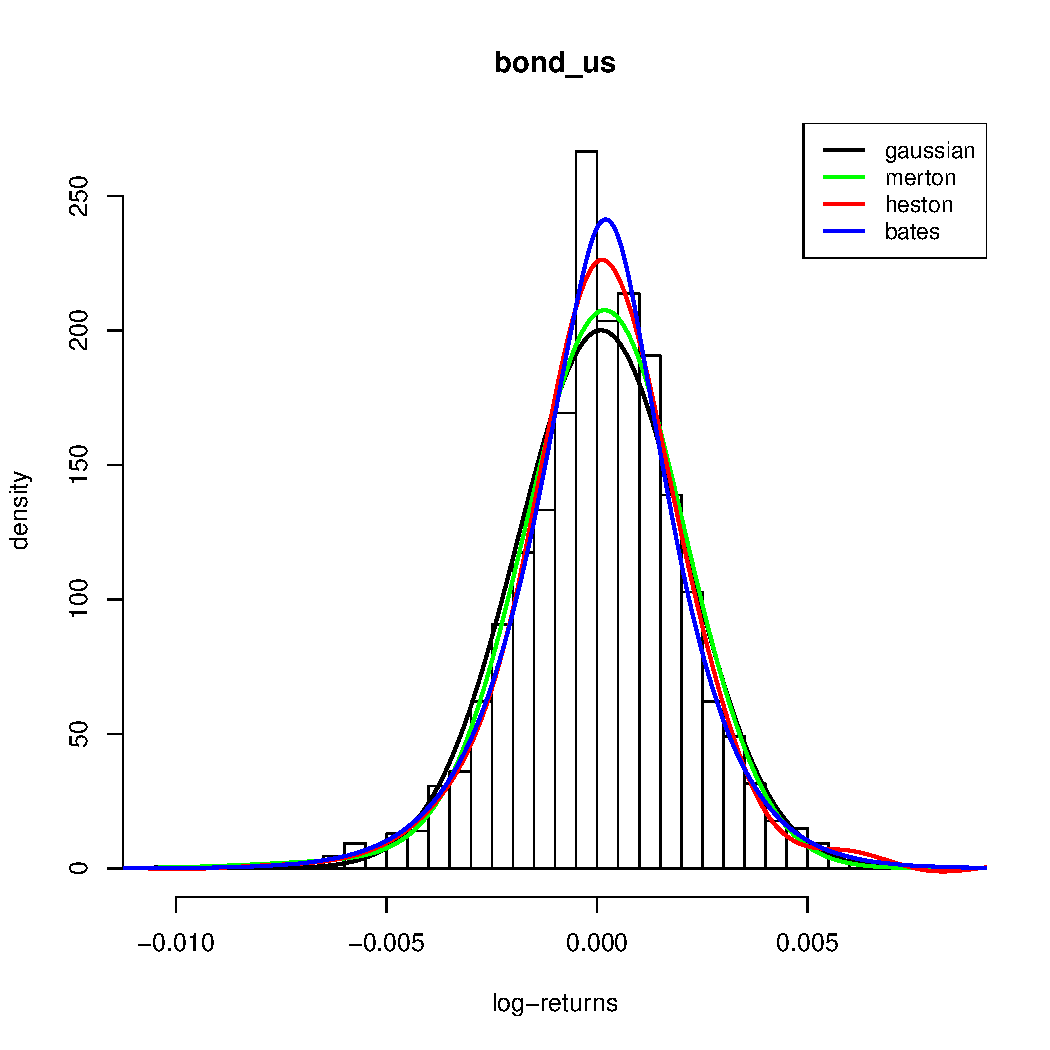
\includegraphics[height=0.3\textheight]{Images/hist_bond_us.pdf}
%}
%\subfloat[Bond EUR]{
%	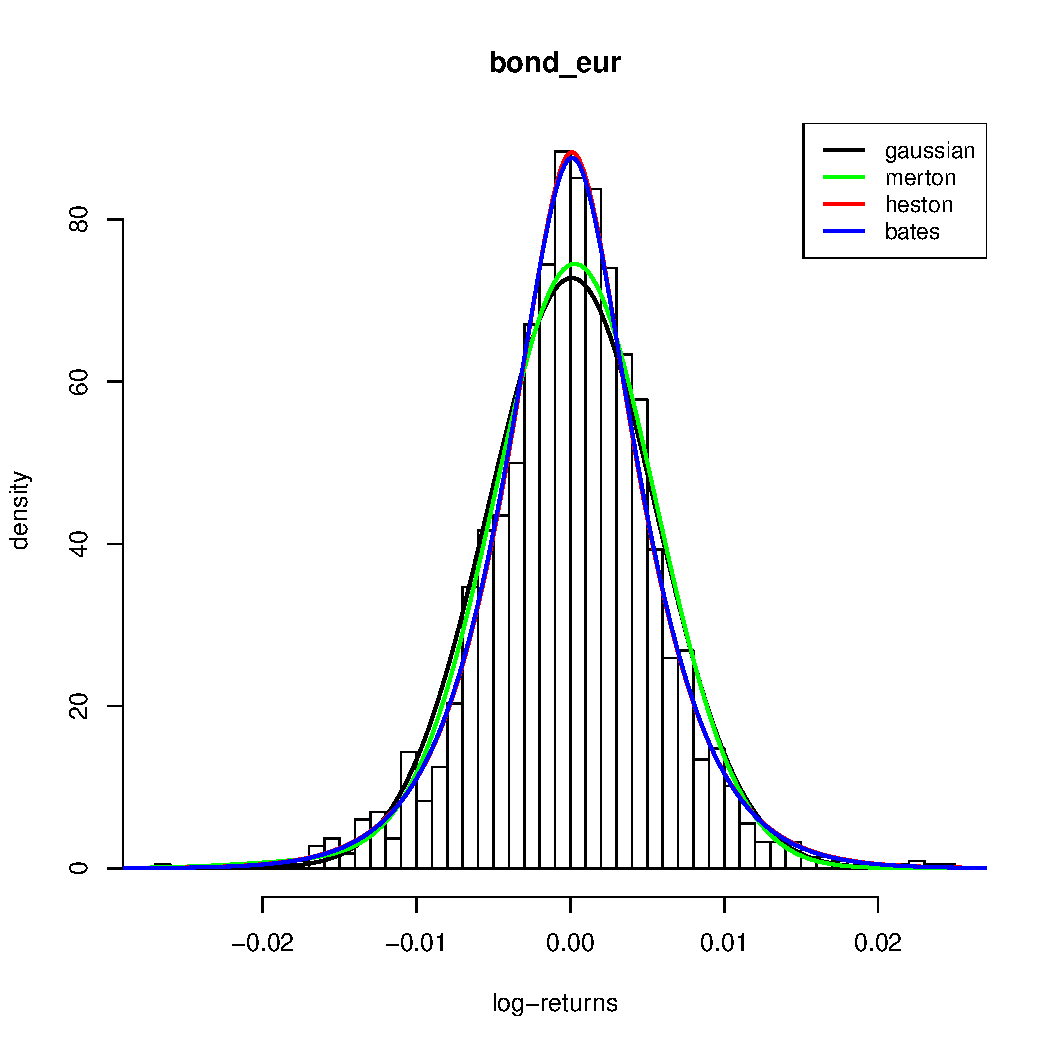
\includegraphics[height=0.3\textheight]{Images/hist_bond_eur.pdf}
%}
\chapter{Discrete Fourier Transform and FFT}
\label{app:FFT}

The Fast Fourier Transform is an algorithm that enables us to compute the Discrete Fourier Transform faster. In particular, a \textit{na\"ive} implementation of the DFT requires a number of operations on the order of $\mathcal{O}(N^2)$, where $N$ is the number of points that we use for the discrete transform. An FFT algorithm performs the same computation using $\mathcal{O}(N \log N)$ operations.


 The discrete Fourier transform for a set $u = u_0 , ..., u_{N-1}$ is  represented by $N$ values $x_k$, $k=0, ..., N-1$:
\begin{equation}
\label{eq:dft_single}
	x_k = \sum_{n=0}^{N-1} u_n \:e^{-i  k n 2\pi / N}, \: k= 0, \dots, N-1.
\end{equation}


As we can see, we have to perform $\mathcal{O}(N)$ computations for each $x_k$, for a total of $\mathcal{O}(N^2)$ operations.
The FFT is a smart way to compute the same quantities by dividing $ N = N_1N_2$ into two factors $ N_1$ and $N_2$, computing the DFT for the two smaller samples and then aggregating the results to return the final $N$ values of $x_k$.

The factorization of $N$ can be performed recursively on $N_1$ and $N_2$ as long as they are not primes. The usual approach is thus to take $N=2^m$ as the $m$-th power of 2. 
The most common algorithm is the one by Cooley and Tuckey in \cite{COOLEY_FFT} and is the one that is usually implemented in most computational tools.


In our case, we want to compute the density function $f(x)$ starting from the characteristic function $\phi(u)$:
\begin{equation}
\label{eq:general_pdf_chf}
f(x) = \frac{1}{2\pi}\int_{-\infty}^{+\infty} \phi(iu) e^{i u x} du
\end{equation}
 using the formula in \eqref{eq:dft_single}. To do so we need first to define for which points we want the density to be computed.
 Let us say we want to obtain values of $f(x)$ for $x\in [a, b)$ using a discretization of $N=2^m$ equidistant points.
 Thus we will have $x_k = a + k \Delta x$ where $\Delta x = (b-a)/N$. 
 
The grid for the $u_n$ is computed using $\Delta u = 2 \pi /(N \Delta x)$ and using an interval centred on zero: $u_n = - N/2 + n \Delta u$. This allows us to obtain a formulation that is similar to \eqref{eq:dft_single} and to take advantage of the FFT algorithm, as we will now show.
 
 We first obtain a discretized version of \eqref{eq:general_pdf_chf} by rectangular approximation and then perform some manipulations to arrive at an expression that looks like that of the DFT:
 
 \begin{equation*}
 \begin{split}
 f(x_k) &= \frac{1}{2 \pi} \sum_{n=0}^{N-1} \phi( i u_n) \: e^{i u_n x_k} \Delta u \\
 &= \frac{\Delta u}{2 \pi} \sum_{n=0}^{N-1} \phi\big(i(-N/2 + n \Delta u)\big) \: e^{i (-N/2 + n \Delta u) x_k}  \\
 &= \frac{\Delta u}{2 \pi} \sum_{n=0}^{N-1} \phi\big(i(-N/2 + n \Delta u)\big) \: e^{i n \Delta u x_k} e^{i (-N/2) x_k}\\
 & = \frac{\Delta u}{2 \pi} \sum_{n=0}^{N-1} \phi\big(i(-N/2 + n \Delta u)\big) \: e^{i n \Delta u (a + k \Delta x) } e^{i (-N/2) x_k} \\
 & = \frac{\Delta u}{2 \pi} \bigg[\sum_{n=0}^{N-1} \phi\big(i(-N/2 + n \Delta u)\big) \:e^{i n \Delta u \:a  }\: e^{i n \Delta u \:k \Delta x }\Big] e^{i (-N/2) x_k} \\
 & = \frac{\Delta u}{2 \pi} \bigg[\sum_{n=0}^{N-1} \bigg(\phi\big(i(-N/2 + n \Delta u)\big) \:e^{i n \Delta u\: a  }\bigg)\: e^{i n k 2\pi/N}\Big] e^{i (-N/2) x_k} .\\
 \end{split}
 \end{equation*}
 
 We can see that in the last line the part that is limited by the square brackets has the same form as  \eqref{eq:dft_single} and thus it can be quickly computed using any FFT algorithm.
%If we compute it for $N$ equispaced values of $u$, $u_k = k \Delta u$ and from a similarly equispaced grid of $x$, $x_n = n \Delta x $ we can rewrite \ref{eq:dft_single} as:
%\begin{equation}
%F(u_k) = \sum_{n=0}^{N-1} f(x_n) e^{-i k n  \Delta u  \Delta x} \Delta x, \: k= 0, \dots, N-1
%\end{equation}




\chapter{Coherent Risk Measure}
\label{app:_risk_measure}

Let us define $\mathcal{L}$ the set of general loss distributions (whether they are discrete or continuous it does not matter), and let $\rho$ be a functional defined from $\mathcal{L}$ to $\mathbb{R} \cup \{\infty\}$.

We define $\rho$ to be a \textit{coherent risk measure} if the following four properties hold:

\begin{itemize}
	\item \textit{subadditivity}: $\quad \forall L_1,L_2 \in \mathcal{L}, \quad \rho(L_1+L_2) \leq \rho(L_1)+ \rho(L_2)$.
	\item \textit{positive homogeneity}: $\quad \forall  \alpha \in \mathbb{R}, \forall L \in \mathcal{L},  \quad \rho(\alpha L) =\alpha \rho(L)$.
	\item  \textit{translation invariance}: $\quad \forall  \alpha \in \mathbb{R}, \forall L \in \mathcal{L},  \quad \rho(L+ \alpha) = \rho(L) + \alpha$.
	\item \textit{monotonicity}: $\quad \forall L_1,L_2 \in \mathcal{L} $ such that $L_1 \leq L_2, \quad \rho(L_1) \leq \rho(L_2)$.
\end{itemize}

The interpretation of the last three properties is immediate and it makes sense that a \textit{coherent} risk measure would satisfy them. The subadditivity is instead a little trickier but it is fundamental since negating it would mean that there is no advantage in diversification, which is known not to be true both by everyday experiences and numerical evidences.

The VaR as a measure of risk is not coherent because it lacks the fundamental property of subadditivity.
\chapter{Code excerpts}
\label{app:code}

%
%\usepackage{listings}
%\usepackage[usenames,dvipsnames]{color}    

\lstset{ 
	language=R,                     % the language of the code
	basicstyle=\tiny\ttfamily, % the size of the fonts that are used for the code
	numbers=left,                   % where to put the line-numbers
	numberstyle=\tiny\color{Blue},  % the style that is used for the line-numbers
	stepnumber=1,                   % the step between two line-numbers. If it is 1, each line
	% will be numbered
	numbersep=5pt,                  % how far the line-numbers are from the code
	backgroundcolor=\color{white},  % choose the background color. You must add \usepackage{color}
	showspaces=false,               % show spaces adding particular underscores
	showstringspaces=false,         % underline spaces within strings
	showtabs=false,                 % show tabs within strings adding particular underscores
	frame=single,                   % adds a frame around the code
	rulecolor=\color{black},        % if not set, the frame-color may be changed on line-breaks within not-black text (e.g. commens (green here))
	tabsize=2,                      % sets default tabsize to 2 spaces
	captionpos=b,                   % sets the caption-position to bottom
	breaklines=true,                % sets automatic line breaking
	breakatwhitespace=false,        % sets if automatic breaks should only happen at whitespace
    keywordstyle=\color{black},      % keyword style
	commentstyle=\color{YellowGreen},   % comment style
	stringstyle=\color{ForestGreen}      % string literal style
} 

\section{Correlation analysis}
Function to perform the Permutation test:
\begin{lstlisting}

PermutationTestCorr = function(x,y=0, N=2000){
	# Two sided permutation test for correlation
	# H0: rho = 0   vs    H1: rho!=0
	# Input
	#   x: first variable values
	#   y: second variable values
	
	if (!is.null(dim(x)[2])){
		if ( dim(x)[2] == 2){
		y=x[,2]
		x=x[,1]
		}
	}
	else if (length(x)!=length(y)){
		stop("Error: samples should have same size.")
	}
	
	n = length(x)
	
	r_sample= cor(x,y)
	
	larger = 0
	for(i in 1:N){
		y_perm = y[sample(n,n)]
		r_perm = cor(x,y_perm)
		if (abs(r_sample)<abs(r_perm))
			larger = larger+1
	}
	# p-value is the percentage of r_perm absolutely greater than r_sample
	p = larger/N
	return(p)
} 
\end{lstlisting}

\section{Merton, Heston and Bates  calibration}

\subsection{General structure for full calibration}
\bigskip
\noindent
Script to calibrate the \texttt{N\_assets} Merton model, similar structure also for the other models, just different functions for parameters  and model correlation calibration:
\begin{lstlisting}
### Loading daily log-returns dataset
load("returns.Rda")
attach(my_returns)


N = dim(my_returns)[1] #total number of observations
N_assets= 16
dt = 1/255

# matrix to store the parameters for each asset
full_results = matrix(0, nrow = N_assets, ncol = 5) 
rownames(full_results) = colnames(my_returns)[2*(1:N_assets)]
colnames(full_results) = c("mu", "sigma","theta","delta","lambda")

### Calibrating each single asset model
for (i in 1:N_assets){
	asset = my_returns[,2*i] #contains single asset daily log-returns
	asset_name = colnames(my_returns)[2*i]
	
	# actual calibration function
	calibrated_params = CalibrateMerton(x=matrix(asset[1:N], ncol=1),dt = dt, custom_jump_bounds = T)
	
	full_results[i,]=c(calibrated_params$mu, sqrt(calibrated_params$S), calibrated_params$theta, calibrated_params$delta, calibrated_params$lambda)
}


#### Calibrating model Correlation matrix

n=16
# sample corr matrix for comparison
corr_matrix = cor(my_returns[,2*(1:n)])

beg = Sys.time()
# model correlation matrix
model_corr_mat = calibrate_full_correlation_merton(sample_corr_matrix = corr_matrix, Nasset = n, 
						mu =full_results[1:n,1] , vol = full_results[1:n,2], mu_j = full_results[1:n,3], 
						sigma_j = full_results[1:n,4], lambda = full_results[1:n,5], dt = 1/255,final_t = 2, 
						Nsim = 1000)
# show computation time
Sys.time() - beg

# print both matrices to screen for comparison
model_corr_mat
corr_matrix[1:n,1:n]
\end{lstlisting}


\subsection{Single asset calibration}
\bigskip
\noindent
Function that performs the calibration for a single asset Merton, only differences in the Heston and Bates cases is the objective function in the optimizers that are respectively  \texttt{heston\_negloglik} and \texttt{bates\_negloglik}
\begin{lstlisting}
CalibrateMerton=function(x, n, dt, trace = 10, custom_jump_bounds =T){
	
	library(DEoptim)
	source("MultivariateMertonModel.R")
	
	if(custom_jump_bounds){
		min_jump = rep(0,n)
		max_jump = rep(0,n)
		
		alpha_max = 0.995 # quantile for max jump
		alpha_min = 0.999 # quantile for min jump
		for (i in 1:n) {
			min_jump[i] = 2*quantile(x= x[,i], probs = 1-alpha_min)
			max_jump[i] = quantile(x= x[,i], probs = 1-alpha_max)
		}
	}
	else{
		min_jump = rep(-0.1,n) # default jumps at -10%
		max_jump = rep(-1,n)
	}
	
	# Obtaining bounds from function BoundsCreator
	bounds_nocommon = BoundsCreator(custom_jump_mean = custom_jump_bounds,
	max_jump_mean = max_jump, min_jump_mean = min_jump)
	
	print(rbind(bounds_nocommon$lower, bounds_nocommon$upper))
	
	# First optimization using deoptim
	print("Starting calibration using DEoptim...")
	control_list_deoptim = list(itermax = 50, NP = 10*length(bounds_nocommon$lower), strategy = 6,trace=trace)
	
	
	start_time_deoptim <- Sys.time()
	outDE <- DEoptim(merton_negloglik,  # objective function is the negative log likelihood for Merton
			lower = bounds_nocommon$lower, upper = bounds_nocommon$upper, control = control_list_deoptim, dt = dt, x = x)
	end_time_deoptim <- Sys.time()
	
	# Second and final optimization using nlminb
	print("Starting calibration using nlminb...")
	
	initial=outDE$optim$bestmem
	start_time_nlminb <- Sys.time()
	out_nlminb = nlminb(initial,objective = merton_negloglik,lower = bounds_nocommon$lower,
	upper = bounds_nocommon$upper,dt=dt, x=x,
	control=list(eval.max = 10000,iter.max = 1000, trace = trace))
	print(out_nlminb)
	end_time_nlminb <- Sys.time()
	
	print(paste("DEoptim time:",end_time_deoptim - start_time_deoptim))
	print(paste("nlminb time:", end_time_nlminb - start_time_nlminb))
	print(paste("TOTAL time:", end_time_nlminb - start_time_deoptim))
	
	res = ParametersReconstruction(out_nlminb$par,n=n)
	res[["message"]] = out_nlminb$message
	res[["objective_function"]] = out_nlminb$objective
	res[["total_time"]] = end_time_nlminb - start_time_deoptim
	return(res)
}
\end{lstlisting}


\bigskip
\noindent
Pdf and log-likelihood function for Merton:
\begin{lstlisting}
#Pdf for Merton model
merton_pdf = function(x, dt, mu, sigma, mu_J, sigma_J, lambda){
	# Computes the density of a multivariate merton model returns with idiosyncratic and common jumps
	# ASSUMPTION: in dt time we can only have 0 or 1 jumps in each jump process, so lambda*dt<=1
	#
	# INPUT
	# x:      vector representing at which point to compute the density 
	# mu:     drift of the continuos part 
	# sigma:      covariance of the continuous part 
	# mu_J:  means of the idiosyncratic jump intensity 
	# sigma_J:  volatility of the idiosyncratic jump intensity 
	# lambda:  poisson parameters of the idiosyncratic jump part 
	
	# check on lambdas: 
	ldt =lambda*dt
	if(ldt>=1){
		stop("Error: lambda*dt should be lower than 1 (ideally close to 0).")
	}
	
	mu_adj= mu - sigma^2/2 -lambda*mu_J 
	pdf=(1-ldt)*dnorm(x, mean = mu_adj*dt, sd = sqrt(sigma^2*dt))+ldt *dnorm(x, mean = mu_adj*dt + mu_J, sd = sqrt(sigma^2*dt + sigma_J^2))
	
	return(pdf)
}


merton_negloglik= function(params, x, dt) {
	# x is a matrix [Npoints * n] of all the points for which we compute the likelihood
	
	# reconstruction of parameters:
	mu=params[1]
	sigma = params[2]
	mu_J = params[3]
	sigma_J = params[4]
	lambda = params[5]
	
	# computing pdf on each point and adding
	partial = merton_pdf(x, dt, mu, sigma, mu_J, sigma_J, lambda)
	nll = -sum(log(partial))
	
	# last check on result
	if (is.nan(nll) | is.na(nll) | is.infinite(nll)) {
		nll = 1e10
	}
	
	return(nll)
}
\end{lstlisting}


\bigskip
\noindent
Pdf, unconditional chf and negative log-likelihood functions for Heston:

\begin{lstlisting}
# Pdf for Heston usinf FFT
pdfHeston_fft = function(x, dt, r, k, theta, sigma_V, rho, N = 2^10){
	# Auxiliary function
	aux_chf = function(u,tau = dt, r_cf = r, k_cf = k,vT = theta, sigma = sigma_V, rho_cf = rho ){
		uncond_cfHeston(u,tau ,r_cf ,k_cf,vT,sigma,rho_cf)
	}
	
	min_x = min(x, -1)
	max_x = max(x, 1)
	eps = 0.01
	
	# Function that performs the inversion by using the FFT algorithm
	pdf = characteristic_function_to_density(aux_chf,N, min_x-eps, max_x+eps)
	
	pdf_xx = interp1(pdf$x, pdf$density, x,method = 'spline')
	return(pdf_xx)
}


# Neg logLikelihood function for Heston
heston_negloglik= function(params, x, dt, check_feller=TRUE){
	r = params[1]
	k =params[2]
	theta = params[3]
	sigma_V = params[4]
	rho = params[5]
	
	pdfs= pdfHeston_fft(x=x, dt=dt,
	r = r, k=k, theta=theta, sigma_V = sigma_V, rho = rho)
	
	to_sum = log(pdfs)
	nll = -sum(to_sum)
	
	if (is.nan(nll) | is.na(nll) | is.infinite(nll)) {
		nll = 1e10
	}
	
	return(nll)
}



# Unconditional chf for Heston
uncond_cfHeston = function(om, tau, r, k, vT, sigma, rho){
	
	if (sigma < 1e-08) 
		sigma <- 1e-08
	
	om[which(om==0)]= 1e-8
	d <- sqrt((rho * sigma * (0+1i) * om - k)^2 + sigma^2 * ((0+1i) *om + om^2))
	g <- (k - rho * sigma * (0+1i) * om - d)/(k - rho * sigma * (0+1i) * om + d)
	
	# to avoid nan due to 0/0
	g[which((k - rho * sigma * (0+1i) * om - d)==0)]=0
	
	A <- 1i*om *r * tau + vT * k/(sigma^2) * ((k - rho * sigma * (0+1i) * om - d) * tau - 2 * log((1 - g * exp(-d * tau))/(1 - g)))
	B <- (k - rho * sigma * (0+1i) * om - d)/sigma^2 * (1 - exp(-d * tau))/(1 - g * exp(-d * tau))
	
	w = 2*k/sigma^2
	nu = 2*k*vT/sigma^2
	
	res = exp(A)*(w/(w-B))^nu
	return(res)
}
\end{lstlisting}

\bigskip
\noindent
Pdf, unconditional chf and negative log-likelihood functions for Bates:
\begin{lstlisting}
# pdf for Bates using FFT
pdfBates_fft = function(x,  dt,  r, k,theta, sigma_V, rho, lambda, mu_j, sigma_j,N=2^12){
	# Auxiliary function
	aux_bates = function( u, tau=dt, r_cf=r, vT=theta, rho_cf=rho, k_cf=k, sigma=sigma_V, lambda_cf=lambda, muJ=mu_j, vJ=sigma_j){
		uncond_cfBates(u,tau, r_cf, vT, rho_cf, k_cf, sigma, lambda_cf, muJ, vJ)
	}
	
	min_x = min(x, -1)
	max_x = max(x, 1)
	eps = 0.1
	
	# Function that performs the inversion by using the FFT algorithm
	pdf = characteristic_function_to_density(aux_bates,N, min_x-eps, max_x+eps)
	
	pdf_xx = interp1( x = pdf$x, y = pdf$density, xi = x, method = 'spline')
	return(pdf_xx)
}
	
	
# Neg logLikelihood function for Bates
bates_negloglik = function(params, x, dt, model="bates", check_feller){
	r = params[1]
	k=params[2]
	theta=params[3]
	sigma_V = params[4]
	rho = params[5]
	mu_j= params[6]
	sigma_j=params[7]
	lambda=params[8]
	
	pdfs= pdfBates_fft(x=x,dt=dt, r=r,k=k, theta=theta,sigma_V=sigma_V,rho =rho,
	mu_j = mu_j, sigma_j = sigma_j, lambda=lambda)
	
	to_sum = log(pdfs)
	nll = -sum(to_sum)
	
	if (is.nan(nll) | is.na(nll) | is.infinite(nll)) {
		nll = 1e10
	}
	
	return(nll)
}
	
# Unconditional chf for Bates
uncond_cfBates= function (om,tau, r, vT, rho, k, sigma, lambda, muJ, vJ)
	{
	if (sigma < 1e-08)
		sigma <- 1e-08
	#sigma <- max(sigma, 1e-04)
	
	om[which(om==0)]= 1e-9
	om1i <- om * (0+1i)
	
	d <- sqrt((rho * sigma * om1i - k)^2 + sigma^2 * (om1i + om^2))
	g <- (k - rho * sigma * om1i - d)/(k - rho * sigma * om1i + d)
	
	# to avoid nan due to 0/0
	g[which((k - rho * sigma * (0+1i) * om - d)==0)]=0
	
	cf1 <- om1i * ( r * tau) 
	cf2 <- vT * k/(sigma^2) * ((k - rho * sigma * om1i - d) * tau - 2 * log((1 - g * exp(-d * tau))/(1 - g)))
	cf_jump <- -lambda * muJ * om1i * tau + lambda * tau * ((1 + muJ)^(om1i) * exp(vJ * (om1i/2) * (om1i - 1)) - 1)
	
	A = cf1+cf2+cf_jump
	B = 1/sigma^2 * (k - rho * sigma * om1i - d) * (1 - exp(-d * tau))/(1 - g * exp(-d * tau))
	
	w = 2*k/sigma^2
	nu = 2*k*vT/sigma^2
	
	res = exp(A)*(w/(w-B))^nu
	return(res)
}
\end{lstlisting}



\subsection{Model correlation calibration}
\bigskip
\noindent
Functions to perform the model correlation matrix calibration in the Merton case:

\begin{lstlisting}
library(MASS)

# Performs the simulation of Merton model given the parameters in input
simulate_mv_merton = function(Nasset=length(mu), mu, vol=NA, mu_j, sigma_j, lambda, CorrMatrix=matrix(NA), CovMatrix = matrix(NA),
x0=rep(0,Nasset), dt=1/255, final_t=1, Nsim=100){

if(is.na(CorrMatrix[1])& Nasset==1){
CorrMatrix=matrix(1)
}
if(is.na(CovMatrix[1])){
if (is.na(vol[1]) | is.na(CorrMatrix[1])){
stop("Need to specify volatilities and Correlation Matrix, or only Covariance Matrix")
}
}
if(is.na(vol[1]) & is.na(CorrMatrix[1])){
CorrMatrix = cov2cor(CovMatrix)
vol = sqrt(diag(CovMatrix))
}

if (Nasset!=length(mu) | Nasset!=length(x0) |
Nasset!=length(mu_j) | Nasset!=length(sigma_j) | Nasset!=length(lambda)){
#print(paste(Nasset,length(mu),length(x0),length(mu_j),length(sigma_j),length(lambda)))
stop("Wrong dimension of parameters or initial values.")
}

Nstep = ceil(final_t / dt)
sim_x =array(0, dim = c(Nsim, Nstep+1, Nasset), dimnames = list(NULL,NULL,paste0("X_",1:Nasset)))
for (m in 1:Nasset) {
sim_x[,1,m] = x0[m]
}

for (i in 1:(Nstep)) {
z = mvrnorm(n = Nsim,mu=rep(0,Nasset) ,Sigma =CorrMatrix)
for (m in 1:Nasset) {
dq = rpois(Nsim, lambda = lambda[m]*dt)
# jump = rnorm(Nsim, mean = log(1+mu_j[m]) - 0.5*sigma_j[m]^2, sd = sigma_j[m])
jump = rnorm(Nsim, mean = mu_j[m], sd = sigma_j[m])
sim_x[, i+1,m] = sim_x[,i,m] + (mu[m] - vol[m]^2*0.5 -lambda[m]*mu_j[m] )* dt + vol[m]*sqrt(dt)*z[,m] + dq * (jump)
}
}

res_x = lapply(seq(dim(sim_x)[3]), function(t) sim_x[ , , t])
names(res_x) = paste0("x_",1:Nasset)
return( res_x)
}



# Computes correlation matrix from given simulation result
correlation_MC_estimation = function( simulation_result){
# simulation result should be a n-asset simulation output of simulate_mv_merton
# NOTE: correlation is computed on the log returns in [t,t+dt] 

Nasset = length(simulation_result) 
Nsim = dim(simulation_result[[1]])[1] 

if( Nasset == 2 ){
sumcorr= 0
for (k in 1:Nsim) {
# correlation of log-returns in path k
sumcorr = sumcorr + cor(diff(simulation_result[[1]][k,]), diff(simulation_result[[2]][k,]))
}
res = sumcorr/Nsim      # average correlation on different scenarios
}
else if (Nasset > 2){
corr_matrix = diag(nrow = Nasset) # Identity matrix 
for ( i in 1:(Nasset-1)) {
for (j in (i+1):Nasset) {
sumcorr = 0
for (k in 1:Nsim) {
sumcorr = sumcorr + cor(diff(simulation_result[[i]][k,]), diff(simulation_result[[j]][k,]))
}
corr_matrix[i,j] = sumcorr/Nsim
corr_matrix[j,i] = sumcorr/Nsim
}
}
res = corr_matrix
}
else{
stop("Need at least 2 assets to compute correlation.")
}
return(res)
}

# Computes correlation for 2 assets from initial and model parameters [ used in model correlation calibration]
expected_model_correlation_merton = function(model_corr, mu, vol, mu_j, sigma_j, lambda,
x0, dt=1/255, final_t=1, Nsim){
simulated = simulate_mv_merton(Nasset = 2, mu, vol, mu_j, sigma_j, lambda, matrix(c(1,model_corr, model_corr,1),ncol=2),
x0=x0, dt=dt, final_t=final_t, Nsim = Nsim)
rho_MC = correlation_MC_estimation(simulated)
rho_MC
}

# Calibrates the model correlation of a 2-asset Merton given the sample corr
calibrate_correlation_merton = function(sample_corr,Nasset=length(mu), mu, vol, mu_j, sigma_j, lambda, x0=c(0,0), dt=1/255, final_t=1, Nsim=100){

if (Nasset!=length(mu) | Nasset!=length(x0) |
Nasset!=length(mu_j) | Nasset!=length(sigma_j) | Nasset!=length(lambda)){
stop("Wrong dimension of parameters or initial values.")
}

f_to_be_solved = function(model_corr,  sample_corr, ...){
expected_model_correlation_merton(model_corr=model_corr, ...) - sample_corr
}

res = uniroot(f=f_to_be_solved, interval =c(-1,1),
sample_corr = sample_corr,
mu = mu, vol=vol, mu_j=mu_j, sigma_j=sigma_j, lambda = lambda,
x0=x0, dt=dt, final_t=final_t, Nsim=Nsim,
trace = 3)

return(res$root)
}



# Calibrates the n by n correlation matrix for a n-asset model by iterating on all pairs of assets
calibrate_full_correlation_merton = function(sample_corr_matrix, Nasset=length(mu), mu, vol, mu_j, sigma_j, lambda, x0=rep(0,Nasset), dt=1/255, final_t=1, Nsim=500){

if (Nasset!=length(mu) | Nasset!=length(x0) |
Nasset!=length(mu_j) | Nasset!=length(sigma_j) | Nasset!=length(lambda)){
#print(paste(Nasset,length(mu),length(x0),length(mu_j),length(sigma_j),length(lambda)))
stop("Wrong dimension of parameters or initial values.")
}

# create identity matrix
model_corr_matrix = diag(Nasset) 

for (i in 1:(Nasset-1)) {
for (j in (i+1):Nasset) {
print(paste0("Estimating element [", i, ',', j,']'))
upper_val = expected_model_correlation_merton(model_corr = 1, mu=mu[c(i,j)], vol = vol[c(i,j)],
mu_j=mu_j[c(i,j)], sigma_j=sigma_j[c(i,j)], lambda=lambda[c(i,j)], 
x0=x0[c(i,j)], dt=dt, final_t=final_t, Nsim=Nsim) -sample_corr_matrix[i,j]
lower_val = expected_model_correlation_merton(model_corr = -1, mu=mu[c(i,j)], vol = vol[c(i,j)],
mu_j=mu_j[c(i,j)], sigma_j=sigma_j[c(i,j)], lambda=lambda[c(i,j)], 
x0=x0[c(i,j)], dt=dt, final_t=final_t, Nsim=Nsim) -sample_corr_matrix[i,j]
if(upper_val*lower_val < 0){
model_corr_matrix[i,j] =  calibrate_correlation_merton(sample_corr_matrix[i,j], mu=mu[c(i,j)], vol = vol[c(i,j)],
mu_j=mu_j[c(i,j)], sigma_j=sigma_j[c(i,j)], lambda=lambda[c(i,j)], 
x0=x0[c(i,j)], dt=dt, final_t=final_t, Nsim=Nsim)
}
else{
print(paste("Cannot obtain a correlation of", sample_corr_matrix[i,j] , "with given parameters." ))
if(abs(upper_val)>abs(lower_val)){
model_corr_matrix[i,j] = -1
}
else{
model_corr_matrix[i,j] = 1
}
}
model_corr_matrix[j,i] = model_corr_matrix[i,j]
}
}

model_corr_matrix = regularization(model_corr_matrix, method = "jackel")

return(model_corr_matrix)
}

# Performs matrix regularization
regularization = function(mat, method =  'jackel'){
decomp = eigen(mat,symmetric = TRUE)
S = decomp$vectors
eigval = decomp$values

# print("Eigenvalues: ")
# print(eigval)

if(method =="jackel"){
eigval[which(eigval<0)]=0

Lambda = diag(eigval)

t = rep(x=NA, length(eigval))
for (i in 1:length(eigval)) {
t[i] = 1/sum(S[i,]^2 * eigval)
}  
B = sqrt(diag(t)) %*% S %*% sqrt(Lambda)

res = B %*% t(B)
}
else{
eigval[which(eigval<0)]=1e-5
res = S %*% diag(eigval)%*% t(S)
}
res
}
\end{lstlisting}

\bigskip
\noindent
Simulation function for the Bates model (for Heston one only has to set \texttt{lambda} to zero):
\begin{lstlisting}

	simulate_mv_bates = function(Nasset=length(mu), mu, k,theta, sigma_V, rho,mu_j=1, sigma_j=0, lambda=0, CorrMatrix=matrix(1), S0=rep(1,Nasset), V0, dt=1/255, final_t=1, Nsim=100){
	
	if (Nasset!=length(mu) | Nasset!=length(k) | Nasset!=length(theta) | Nasset!=length(sigma_V) | Nasset!=length(rho) | Nasset!=length(S0) | Nasset!=length(V0) | Nasset!=length(mu_j) | Nasset!=length(sigma_j) | Nasset!=length(lambda)){
		stop("Wrong dimension of parameters or initial values.")
	}
	
	# correlation for the brownian motions driving the 2*Nasset vector (S1,V1,S2,V2, ... ,Sn,Vn)
	full_corr = matrix(ncol = 2*Nasset, nrow = 2*Nasset) 
	for (i in 1:Nasset){
	for (j in 1:Nasset) {
	full_corr[2*(i-1)+ c(1,2), 2*(j-1)+ c(1,2)] = correlation_block(rho,CorrMatrix, i,j)
	}
	}
	
	full_corr=regularization(full_corr)
	
	Nstep = ceil(final_t / dt)
	
	sim_x =array(0, dim = c(Nsim, Nstep+1, Nasset), dimnames = list(NULL,NULL,paste0("X_",1:Nasset)))
	sim_V = array(0, dim = c(Nsim, Nstep+1, Nasset),dimnames = list(NULL,NULL,paste0("V_",1:Nasset)))
	
	for (m in 1:Nasset) {
	sim_x[,1,m] = log(S0[m])
	sim_V[,1,m] = V0[m]
	}
	
	for (i in 1:(Nstep)) {
	z = mvrnorm(n = Nsim,mu=rep(0,Nasset*2) ,Sigma =full_corr)
	for (m in 1:Nasset) {
	dq = rbinom(Nsim,size = 1, prob= lambda[m]*dt)
	jump = rnorm(Nsim, mean = log(1+mu_j[m]) - 0.5*sigma_j[m]^2, sd = sigma_j[m])
	V_plus= sim_V[,i,m]*(sim_V[,i,m]>0) # positive part for full truncation
	sim_V[,i+1, m] = sim_V[,i,m] + k[m]*(theta[m] - V_plus)*dt + sigma_V[m]*sqrt(V_plus *dt)*z[,2*m]
	sim_x[, i+1,m] = sim_x[,i,m] + (mu[m] - V_plus*0.5 -lambda[m]*mu_j[m] )* dt + sqrt(V_plus * dt)*z[,2*m-1] + dq * (jump)
	}
	}
	
	res_V = lapply(seq(dim(sim_V)[3]), function(t) sim_V[ , , t])
	names(res_V) = paste0("V_",1:Nasset)
	res_x = lapply(seq(dim(sim_V)[3]), function(t) sim_x[ , , t])
	names(res_x) = paste0("x_",1:Nasset)
	return( list( return = res_x, variance = res_V ))
}
\end{lstlisting}


\section{Optimal allocation}

\subsection{Markowitz efficient frontier}


\noindent
Function to compute the efficient frontier without short-selling (just remove the constraint to obtain the frontier to add the possibility to go short):

\begin{lstlisting}
# Function to compute the efficient frontier without shortselling
EfficientFrontier_constr = function(r,S,full=FALSE, N=100, no_short_sales, max_r=NA, min_r =NA){
	# r: expected returns of the assets
	# S: covariance matrix of the asset returns
	# full: computes only upper section of frontier if FALSE
	# N: how many expected returns to take into consideration
	# no_short_sales: vector containing the indexes of the asset for which it is not possible to go short
	
	require(quadprog)
	
	if (is.na(max_r)){
		max_r = max(r)
	}
	if (is.na(min_r)){
		min_r = min(r)
	}
	
	# number of assets
	n= length(r)
	
	D = 2*S       #times 2 because there is a 1/2 in the implicit formulation
	d = rep(0,n)  # zeros
	
	# Constraint on returns
	A = t(r)
	
	b = 0.0 # expected return that will be iterated to compute frontier
	
	# Constraint on weights: sum(w)=1
	A = rbind(A,rep(1,n))
	b= rbind(b,1)
	
	# Constraint on short selling on given assets
	for (i in no_short_sales){
	A_i = matrix(0,nrow=1,ncol = n)
	A_i[1,i]=1
	A = rbind(A,A_i)
	b = rbind(b,0)
	}
	
	yy= seq(from = min(r), to = max_r,length.out = N+1)
	yy[1] = yy[1]+ 1e-5
	yy[N+1] = yy[N+1] -1e-5
	
	b[1]= yy[1]
	
	xx = rep(0,length(yy))
	for (i in 1:(N+1)) {
		b[1] = yy[i]
		sol = solve.QP(Dmat = D, dvec = (d), Amat = t(A), bvec = t(b), meq = 2)
		xx[i] = sqrt(sol$value)
	}
	
	if (!full){
		min_sigma = min(xx)
		idx = which(yy>=yy[which(xx==min_sigma)])
		xx= xx[idx]
		yy= yy[idx]
	}
	
	res = list(sigma = xx, expected_return=yy)
	return(res)
}
\end{lstlisting}

\subsection{CVaR allocation}

Function to compute the optimal allocation using CVaR as the portfolio risk measure:

\begin{lstlisting}
# Function to compute the optimal allocation using CVaR
OptimalAllocationDailyCVaR= function(daily_return, alpha, target_return, N_rep=1){
	# daily_return: daily return matrix(N_days * N_assets)
	# alpha: level for the CVaR
	# target_return: target return to be reached
	# N_rep: number of times to compute the result in order to then take an average
	
	require(alabama)
	
	N_assets = dim(daily_return)[2]
	
	expected_asset_return = colMeans(daily_return)
	
	solution = list(obj = rep(0,N_rep), params = matrix(rep(0,N_rep*N_assets),ncol = N_assets), expected_ret=rep(0,N_rep))
	
	for (i in 1:N_rep) {
	# creating initial random weights summing to one
	sampled =  runif(N_assets)
	rand_initial = sampled/sum(sampled)
	
	res = auglag(par = rand_initial, fn=daily_ptf_cvar, # objective function
	hin = f_ineq_daily, heq =f_eq_daily, # constraints
	sims=daily_return, alpha = alpha, target_return = target_return, control.outer = list(method = "nlminb", trace = FALSE))
	solution$obj[i]=res$value
	solution$params[i,]=matrix(res$par,ncol = N_assets)
	solution$expected_ret[i]=(sum(res$par*expected_asset_return))
	
	print(paste("Target return:", target_return, "Iteration:", i))
	}
	
	idx = which.min(solution$obj)
	
	return(list(objective = solution$obj[idx], 
	allocation = solution$params[idx,],
	expected_return = solution$expected_ret[idx]))
}

daily_ptf_cvar = function(w,  sims, alpha, target_return){
	daily_loss = 1 - sims%*%w
	sorted_loss = sort(daily_loss,decreasing = FALSE)
	VaR = quantile(x = daily_loss, probs = 1-alpha)
	idx_var = min(which(sorted_loss >= VaR))
	# print(idx_var)
	CVaR = mean(sorted_loss[idx_var:length(sorted_loss)])
	return(CVaR)
}

# Equality constraints
f_eq_daily = function(w, sims, alpha,target_return){
	# weights should sum to 1
	c1 = sum(w)-1 
	N_s = dim(sims)[1]
	# expected return should be the same as target_return
	c3 =  sum(t(sims)%*% matrix(rep(1, N_s),ncol = 1) *w) /N_s - target_return
	return(c(c1, c3))
}

# Inequality constraint
f_ineq_daily = function(w, sims, alpha,target_return){
	# no short-selling, so all weigths should be positive
	return(w)
}
\end{lstlisting}




\backmatter
%----------------------------------------------------------------------------------------
%	BIBLIOGRAPHY
%----------------------------------------------------------------------------------------

\backmatter
%\nocite{*}




\end{document}  